\chapter{Úvod}

\begin{figure}[H]\centering
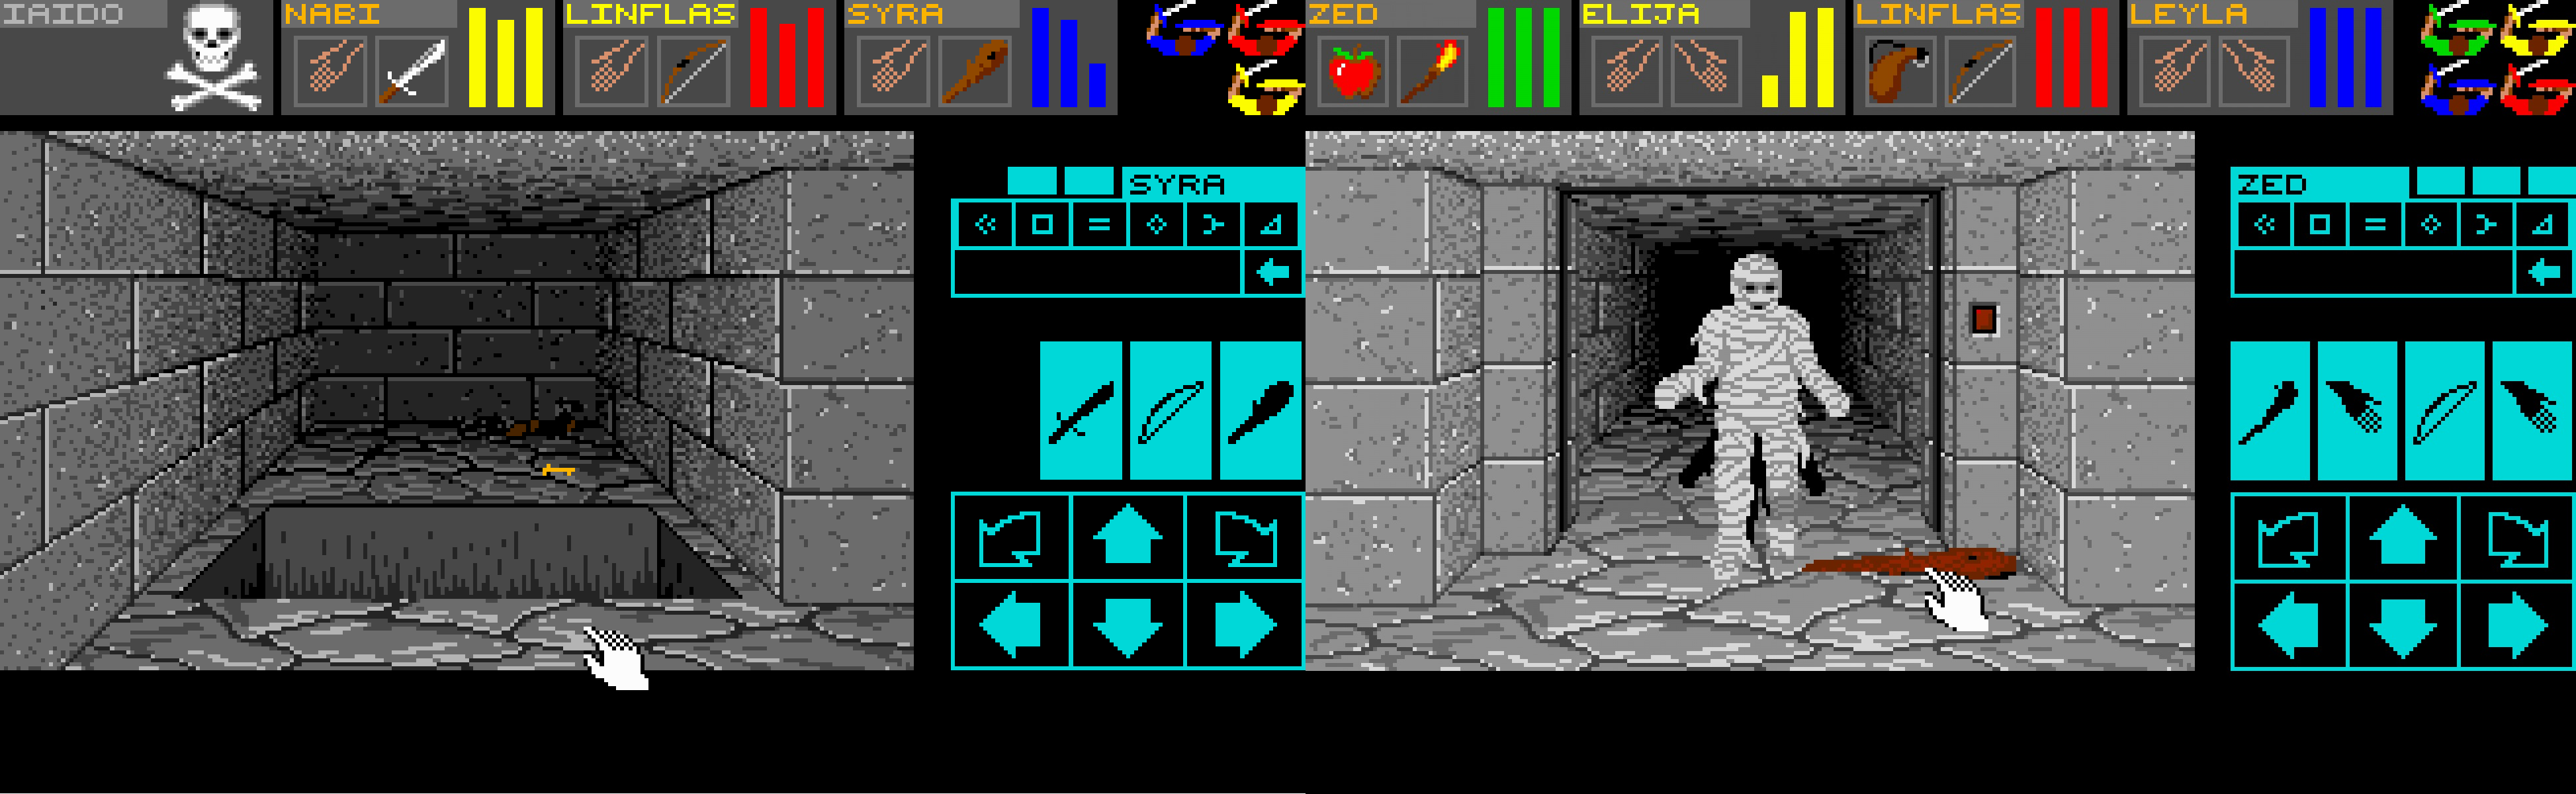
\includegraphics[width=\textwidth]{./img/DM-original-screen.png}
\caption{Screenshot originální hry Dungeon Master}
\label{obr0:uvod}
\end{figure}

Dungeon Master je počítačová hra žánru RPG(role playing game) vyvinuta firmou Faster Then Light v roce 1987.
Byla to první real-time hra tohoto typu s pseudo 3D pohledem a ovládáním pomocí myši. Hráč má k dispozici skupinu až čtyř hrdinů,
s kterými prochází podzemní bludiště a bojuje s nepřáteli\cc{obr0:uvod}. Tito hrdinové se ve hře nazývají šampioni a mohou se 
zdokonalovat v různých dovednostech. 

Bludiště se skládá z několika úrovní uspořádaných vertikálně pod sebou. 
Jednotlivé úrovně pak nemusí být stejně velké a mohou být od sebe různě horizontálně odsazené.
Každá úroveň je tvořena obdélníkovou plochou s pravidelnou mřížkou\cc{obr1:uvod}. Pole vymezena mřížkou nazýváme dlaždice a je jich 
ve hře několik typů, které definují jejích vzhled a funkci. Některé dlaždice lze aktivovat tzv. přepínači. Takové typy dlaždic
jsou například dveře nebo jáma\cc{obr0:uvod}, které lze takto otvírat či zavírat. Přepínače mohou být buď nášlapné na podlaze nebo aktivovatelné
pomocí myši na zdech. Mezi úrovněmi lze sestupovat pomocí dlaždic typu schody.  Dále je možné se teleportovat mezi dlaždicemi, a to i v různých úrovních, pomocí dlaždice
typu teleport. 

\begin{figure}[H]\centering
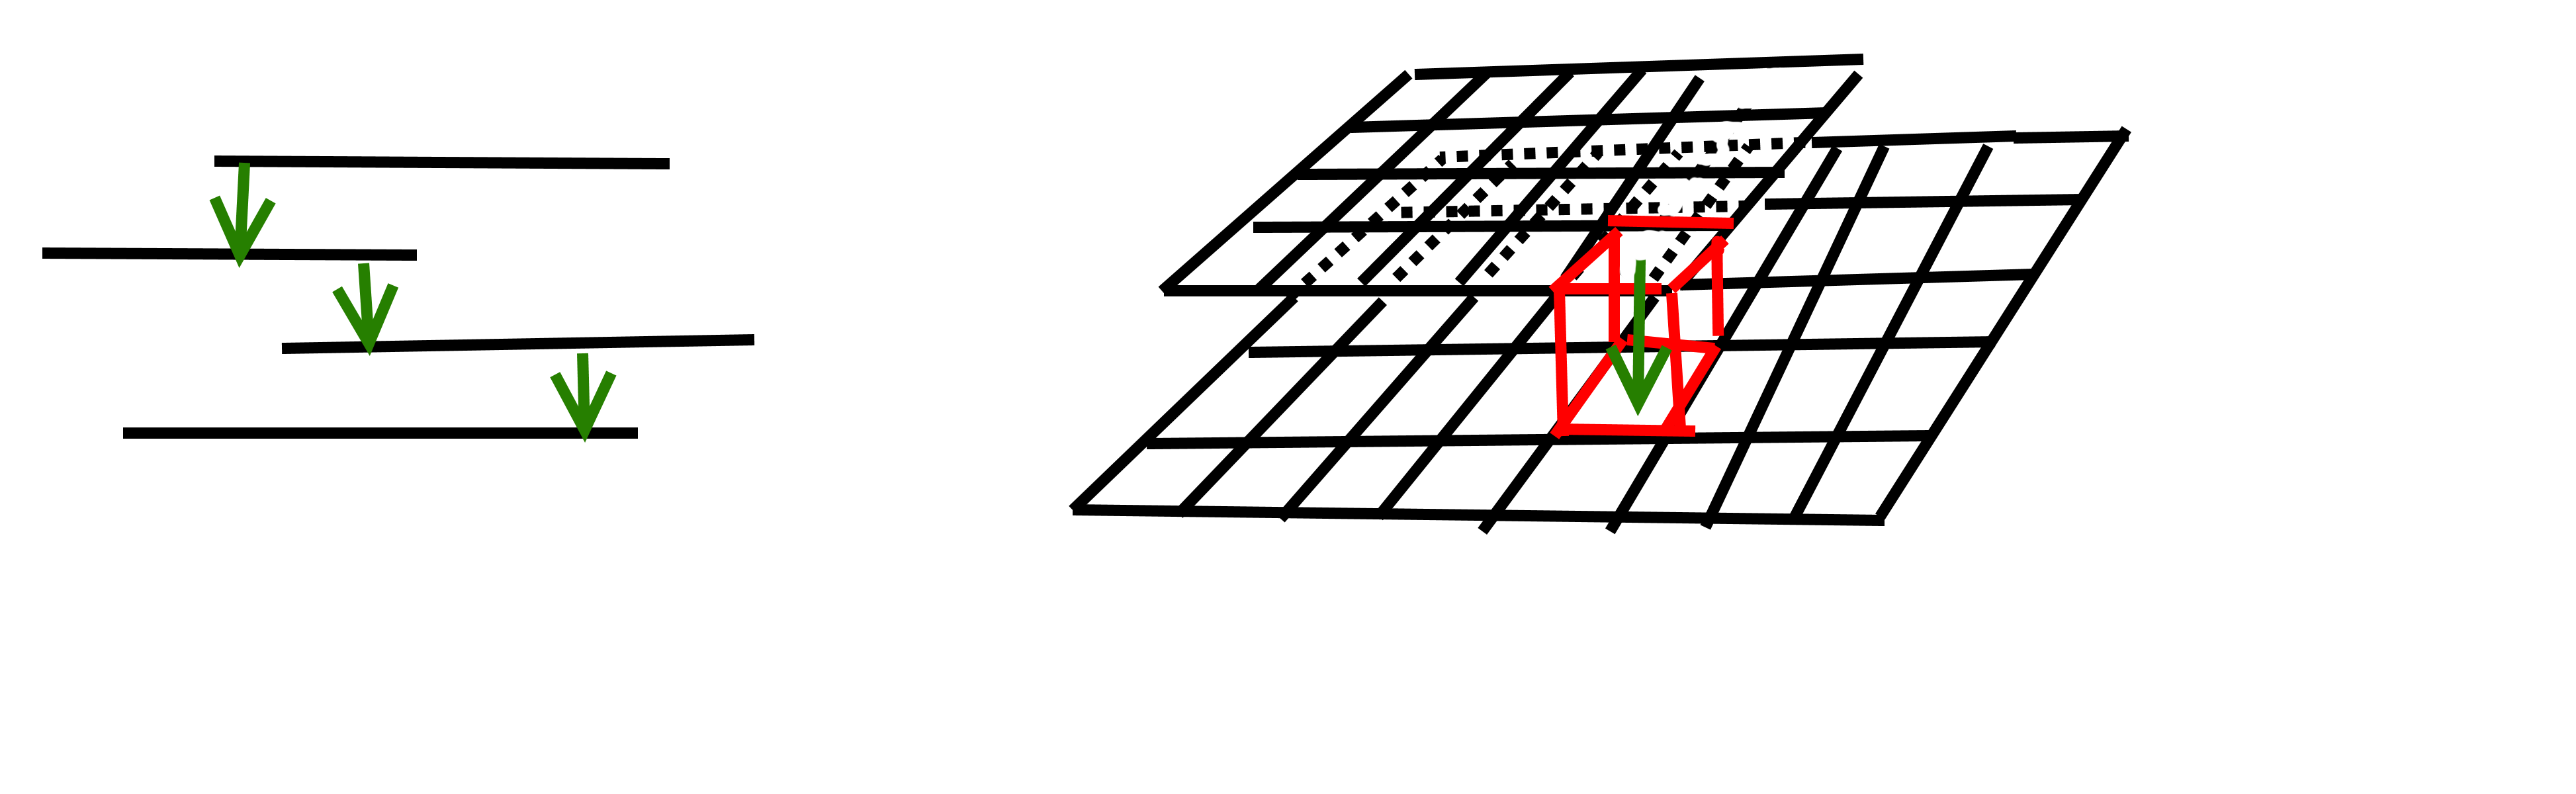
\includegraphics[width=\textwidth]{./img/DM-levels.png}
\caption{Ilustrace uspořádání herních úrovní.}
\label{obr1:uvod}
\end{figure}

Hráč je na začátku postaven do nejvýše položené úrovně, kde si vybere svoji skupinu šampionů. 
Pohyb skupiny mezi dlaždicemi je zcela diskrétní, to znamená, že se nelze se skupinou zastavit mezi dlaždicemi, ale pohyb je vždy dokončen
až na vedlejší dlaždici. Se skupinou je tedy vždy asociována pouze jedna dlaždice. Na dlaždicích pak mohou
být různé předměty, které je možné sbírat. Šampioni mohou s předměty provádět různé akce.
Například se zbraněmi lze bojovat nebo lektvary je možné pít a zlepšit si tak dočasně vlastnosti. Kromě těchto 
akcí může ještě šampion vyvolávat kouzla. Nicméně k tomu potřebuje dostatečnou úroveň odpovídající dovednosti.
Tímto způsobem je možné vytvářet lektvary nebo vyvolávat útočná či obraná kouzla.

Ve hře je celá řada nepřátelský entit. Liší se vzhledem, útokem a pohybem. Pohyb některých entit 
probíhá ještě po hustší mřížce než jsou dlaždice. Každá entita má definovaný prostor dlaždice, který zaujímá. Je to buď prostor
celé dlaždice, polovina či čtvrtina. \cc{obr2:uvod} Pohyb entit je potom opět diskrétní jako v případě hráčovi skupiny, 
ale tentokrát mezi definovanými částmi dlaždic. 

\begin{figure}[H]\centering
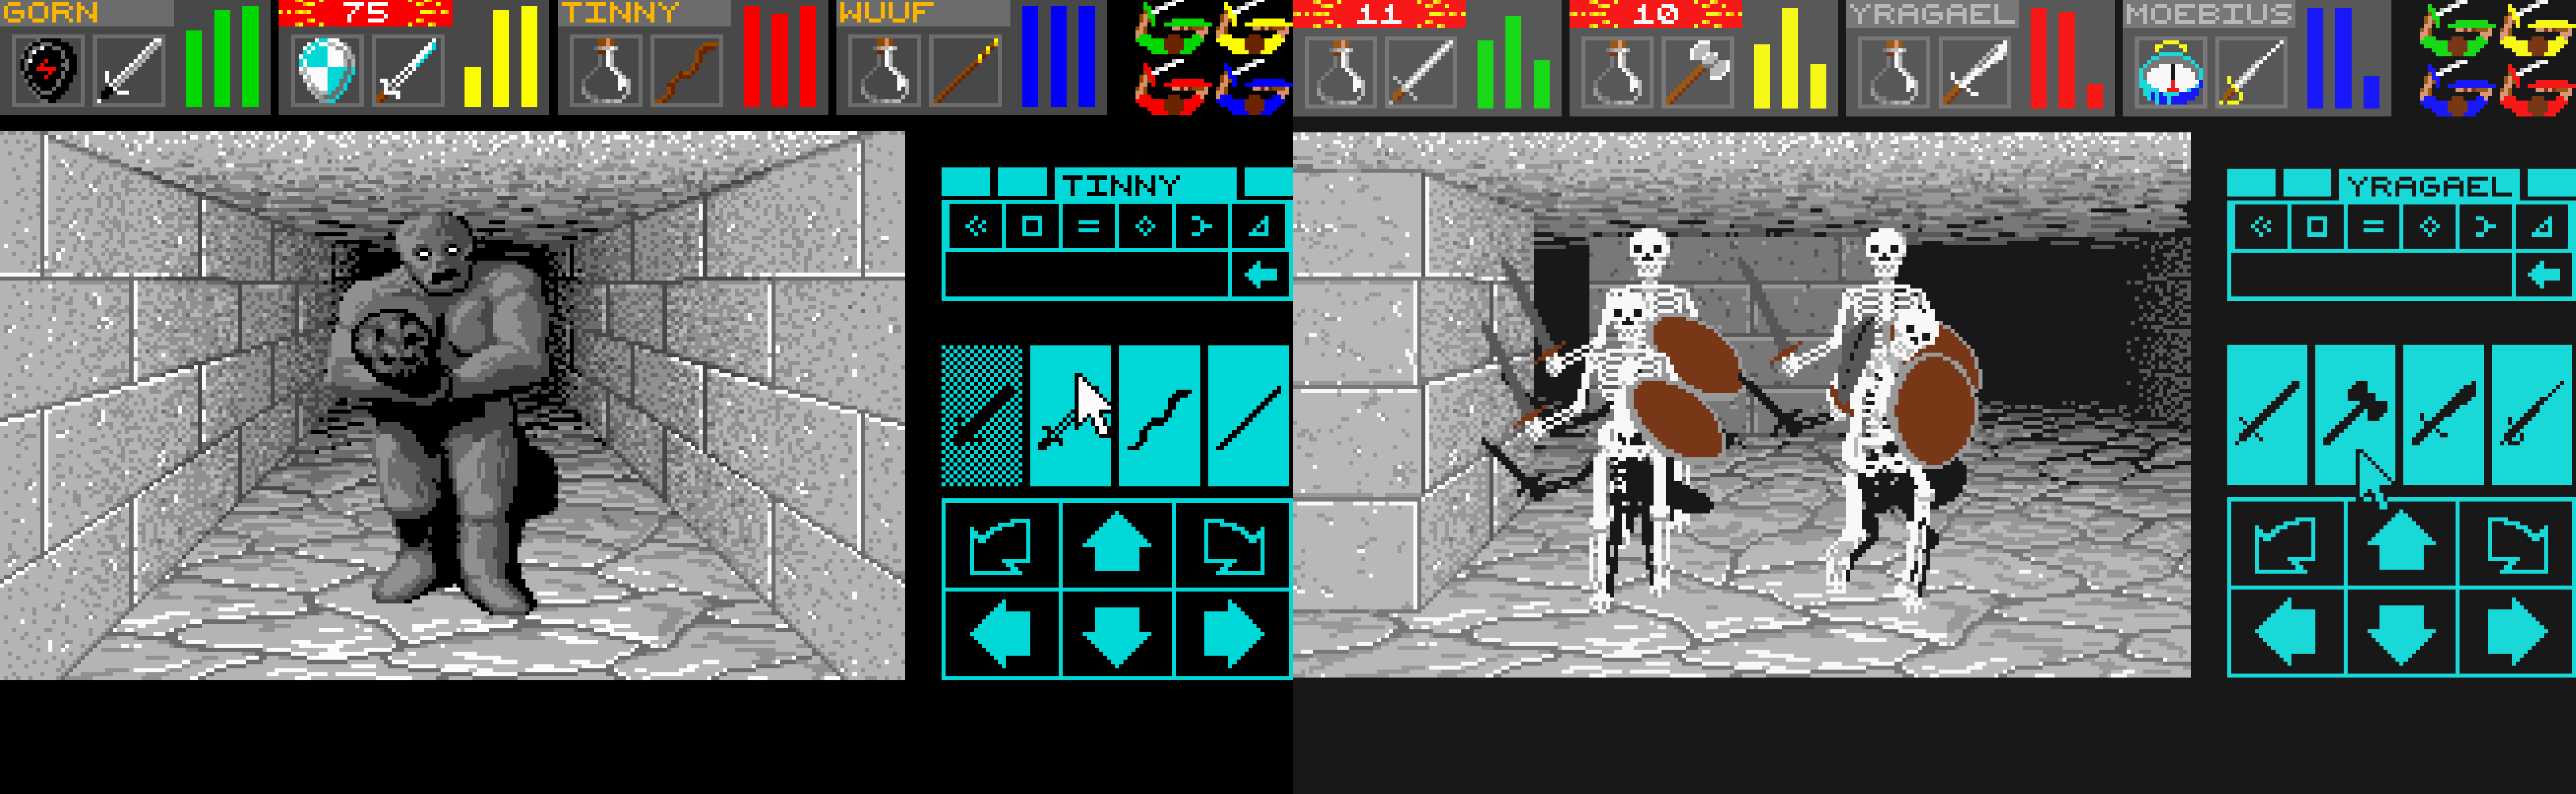
\includegraphics[width=\textwidth]{./img/DM-group-example.png}
\caption{Ilustrace prostorů zaujímaných entitami.}
\label{obr2:uvod}
\end{figure}

Cílem této práce je vytvořit engine pro hru Dungeon Master, tak aby splňovala následující požadavky:
\begin{enumerate}
\item Engine bude naprogramovaný v jazyce C\#.
\item\label{aim-mechanics} Engine bude obsahovat podporu pro funkce a mechaniky vyskytující se ve hře Dungeon Master.
\item\label{aim-extensibility} Bude kladen důraz na dobrý objektový návrh, tak aby byl engine co nejlépe rozšiřitelný a bylo 
	tak možné do enginu dodávat jednoduše nové funkce.
\item\label{aim-builders} Engine bude schopný sestavit herní úrovně podle vstupních dat použitých v originální hře. Nicméně
	bude také poskytovat možnost, dodělat si podporu pro jiné formáty.
\item\label{aim-rendering} Engine bude obsahovat oddělenou zobrazovací vrstvu, tak aby mohl být její výstup jednoduše změněn.
\item Projekt bude cílený pro vzdělávaní, tak aby si studenti mohli vyzkoušet do enginu doprogramovat další funkce.
\end{enumerate}

\chapter{Analýza}

Tato kapitola nejprve blíže popisuje formát a mechaniky originální hry a dále pojednává o postupech a řešeních použitých 
při implementaci nového enginu. Jsou zde popsány jak slepé a nevhodné návrhy, tak návrhy, které se ukázaly 
jako nejvhodnější řešení.

Pro splnění práce bylo v prvé řadě zapotřebí získat vstupní data originální hry Dungeon Master. Nejdůležitější data 
jsou obsažená ve dvou souborech: DUNGEON.DAT a GRAPHICS.DAT. První z nich obsahuje definice herních úrovní a seznamy 
použitých předmětů, přepínačů a nepřátelských entit. Druhý z nich obsahuje konkrétní vlastnosti objektů a entit použitých v prvním souboru. 
Soubor GRAPHICS.DAT pak také obsahuje definicí akcí, vlastnosti kouzel, textury, atd. Později se ukázalo, že pouze data hry nebudou
pro implementaci většiny funkcí dostačující - jedná se například o přesný způsob získávání dovedností šampionů, 
vyvolávání kouzel nebo provádění akcí. Dalším zdrojem jsou dekompilované zdrojové kódy\cite{DMDecompilation} originální hry v jazyce K\&R C.
Tyto zdrojové kódy jsou často náročné na porozumění, nicméně potřebné informace pro dokončení této práce se z nich podařilo získat.

Pro detailnější popis dat Dungeon Masteru si bude dobré nejprve ujasnit vlastnosti a schopnosti šampionů.
Každý šampion má následující vlastnosti:\label{properties-skills}
\begin{itemize}
\item zdraví - určuje kolik útoku šampion vydrží než zemře,
\item výdrž - určuje kolik akcí je schopen šampion vykonat než se unaví, 
\item mana - reprezentuje magickou energii pro vyvolávání kouzel, 
\item zatížení - určuje maximální hmotnost, kterou je šampion schopen unést,
\item síla - hodnota je používána pro výpočet zranění, síly hodu předmětů a maximální výše zatížení,
\item obratnost - zvyšuje pravděpodobnost zásahu nepřítele a pomáhá se vyhnou nepřátelským útokům,
\item moudrost - je to vlastnost důležitá pro kouzelníky a kněze, určuje rychlost obnovy many,
\item vitalita - určuje rychlost obnovy zdraví a výdrže,
\item odolnost proti magii - snižuje účinnost magických útoků,
\item odolnost proti ohni - snižuje účinnost ohnivých útoků,
\item hodnota jídla a vody - pomocí těchto hodnot je obnovována výdrž a zdraví
\item štěstí - zvyšuje či snižuje pravděpodobnost provedení akce.
\end{itemize}

Každý šampion má ve hře čtyři základní dovednosti a to bojovník, ninja, kněz a kouzelník.
Kromě základních dovedností má šampion ještě šestnáct skrytých dovedností, které nejsou hráči zobrazeny.
Každá z těchto skrytých dovedností náleží k nějaké ze základních dovedností.
Jak moc daný šampion disponuje danou dovedností určuje úroveň dovednosti. 
Tato úroveň lze navyšovat pomocí zkušeností, které lze získat souboji nebo prováděním akcí. Každá
akce pak může navyšovat zkušenosti pro jinou dovednost. Pokud jsou v některé ze skrytých dovedností 
získány zkušenosti, dostane odpovídající zkušenosti i její základní dovednost. Po získání dostatečného
počtu zkušeností v nějaké dovednosti, získá šampion v této dovednosti novou úroveň. Nová úroveň potom
navýší určité vlastnosti šampiona. Přesné hodnoty potřebných zkušeností a navyšovaných vlastností pro 
odpovídající dovednosti jsou pevně stanovené ve zdrojových kódech hry.

\section{Vstupní data pro herní úrovně}\label{dungeon-objects}

Originální hra má herní úrovně definované v binárním souboru DUNGEON.DAT. Formát tohoto souboru nebyl tvůrci nikdy zveřejněn,
nicméně kolem hry se vytvořila početná komunita, která k němu dokumentaci\cite{TechnicalDocumentationFontanel05} vytvořila.
Tuto dokumentaci jsme použili k porozumění obsahu souboru. Následuje stručný popis zmíněného souboru, pro 
kompletní dokumentaci navštivte přímo stránky dokumentace.

Soubor DUNGEON.DAT obsahuje jednotlivé herních úrovně a objekty v nich obsažené. Nejprve definuje základní 
vlastnosti o každé herní úrovni. První z nich jsou rozměry dané úrovně, tj. počet dlaždic na šířku a výšku. Dále
definuje obtížnost úrovně, která je použita pro výpočet získaných zkušeností nebo zdraví nepřátelských entit. Každá úroveň má
také určené použité podmnožiny dekorací na zdech, dveřích a přepínačích. Dekorace jsou v originální hře identifikovány čísly, která
jsou napevno zabudovaná v kódu hry. Některé dekorace tak mohou mít ještě speciální význam, který je identifikován
pouze podle zmíněného číselného identifikátoru. Jedná se například o dekorace s výklenky, které mohou být umístěné na zdech.
V tomto případě originální herní engine rozpozná, že lze na dané místo vkládat předměty.

Pomocí přepínačů lze dlaždicím zaslat zprávu, na kterou může cílová dlaždice reagovat. Zpráva obsahuje akci a datovou položku. 
Akce dlaždici říká, zda se má aktivovat či deaktivovat. Co daná datová položka znamená si určuje každý typ cílové dlaždice sám. 
Originální hra pak pracuje s následujícími typy dlaždic:
\begin{itemize}
\item Zeď - zajišťuje zobrazování stěn a nelze na ni vstoupit. Pro každou stěnu(sever, východ, jih, západ - viz obr. \ref{wall:analyza}) dlaždice zdi
	je určeno, zda může mít tzv. náhodnou dekoraci. Pokud ji může mít, engine podle náhodného generátoru
	určí jaká to bude (případně žádná). Každá strana může obsahovat přepínač, který si může do zdi uložit předměty.
	Pokud má některá strana zdi dekoraci výklenku, jsou v něm zobrazeny předměty uložené ve zdi.
	Na stěnách zdi ještě mohou být popisky, které lze zobrazovat nebo skrývat pomocí zaslání zprávy. Aktivační zpráva 
	popisek zviditelní a deaktivační skryje. Datová položka zprávy zde určuje, pro kterou ze stěn zdi je zpráva určena.

\item Podlaha - Po těchto dlaždicích se hráč běžně pohybuje se svoji skupinou. Obdobně jako u stran zdí může definovat,
	zda zobrazuje na podlaze náhodnou dekoraci. Podlaha dále může mít nášlapný přepínač. Dlaždice obsahuje čtyři pozice,
	na které lze pokládat předměty. Tyto pozice vzniknou rozdělením plochy dlaždice na čtvrtiny \cc{floor:analyza}.


\item Jáma - Jáma může být buď otevřená nebo zavřená. Nicméně lze na ni vždy vstoupit a pokud je otevřená 
	hráč spadne s svoji skupinou o úroveň níže. Pád může být i přes několik úrovní. Živé objekty pak po
	dopadu obdrží zranění. Přijmutím aktivační zprávy se jáma otevře a deaktivační se zavře.

\item Schody - Po této dlaždici se může hráč dostat o úroveň výše resp. níže.

\item Dveře - Na těchto dlaždicích je vždy objekt dveře. Na dlaždici lze vstoupit pouze v případě, že jsou dveře
	otevřeny. Otevření je možné provést aktivační zprávou či pomocí tlačítka - pokud ho dveře obsahují. 
	Některé dveře lze také rozbít útokem, to si ale definuje již samotný objekt dveří.

\item Teleport - Tyto dlaždice obsahují objekt teleport, který určuje, které objekty dokáže přenést. Mohou to být
	předměty, hráčova skupina nebo nepřátelské entity. Po vstupu resp. vložení objektu na dlaždici, je objekt teleportován, pokud
	je odpovídajícího typu. Příjem aktivační resp. deaktivační zprávy aktivuje resp. deaktivuje teleport.

\item Iluze zdi - Tato dlaždice může být buď iluze zdi a nebo otevíratelná zeď. V obou případech je vizuálně neodlišitelná
	od dlaždice typu zdi. V prvním případě je možné na dlaždici vstoupit vkročením do zdi. V druhém případě lze
	zeď odstranit pomocí zaslání odpovídající zprávy na dlaždici. Aktivační zpráva otevře zeď, deaktivační zavře.
\end{itemize}

	\begin{figure}[H]
    \centering
    \begin{subfigure}[b]{0.45\textwidth}
        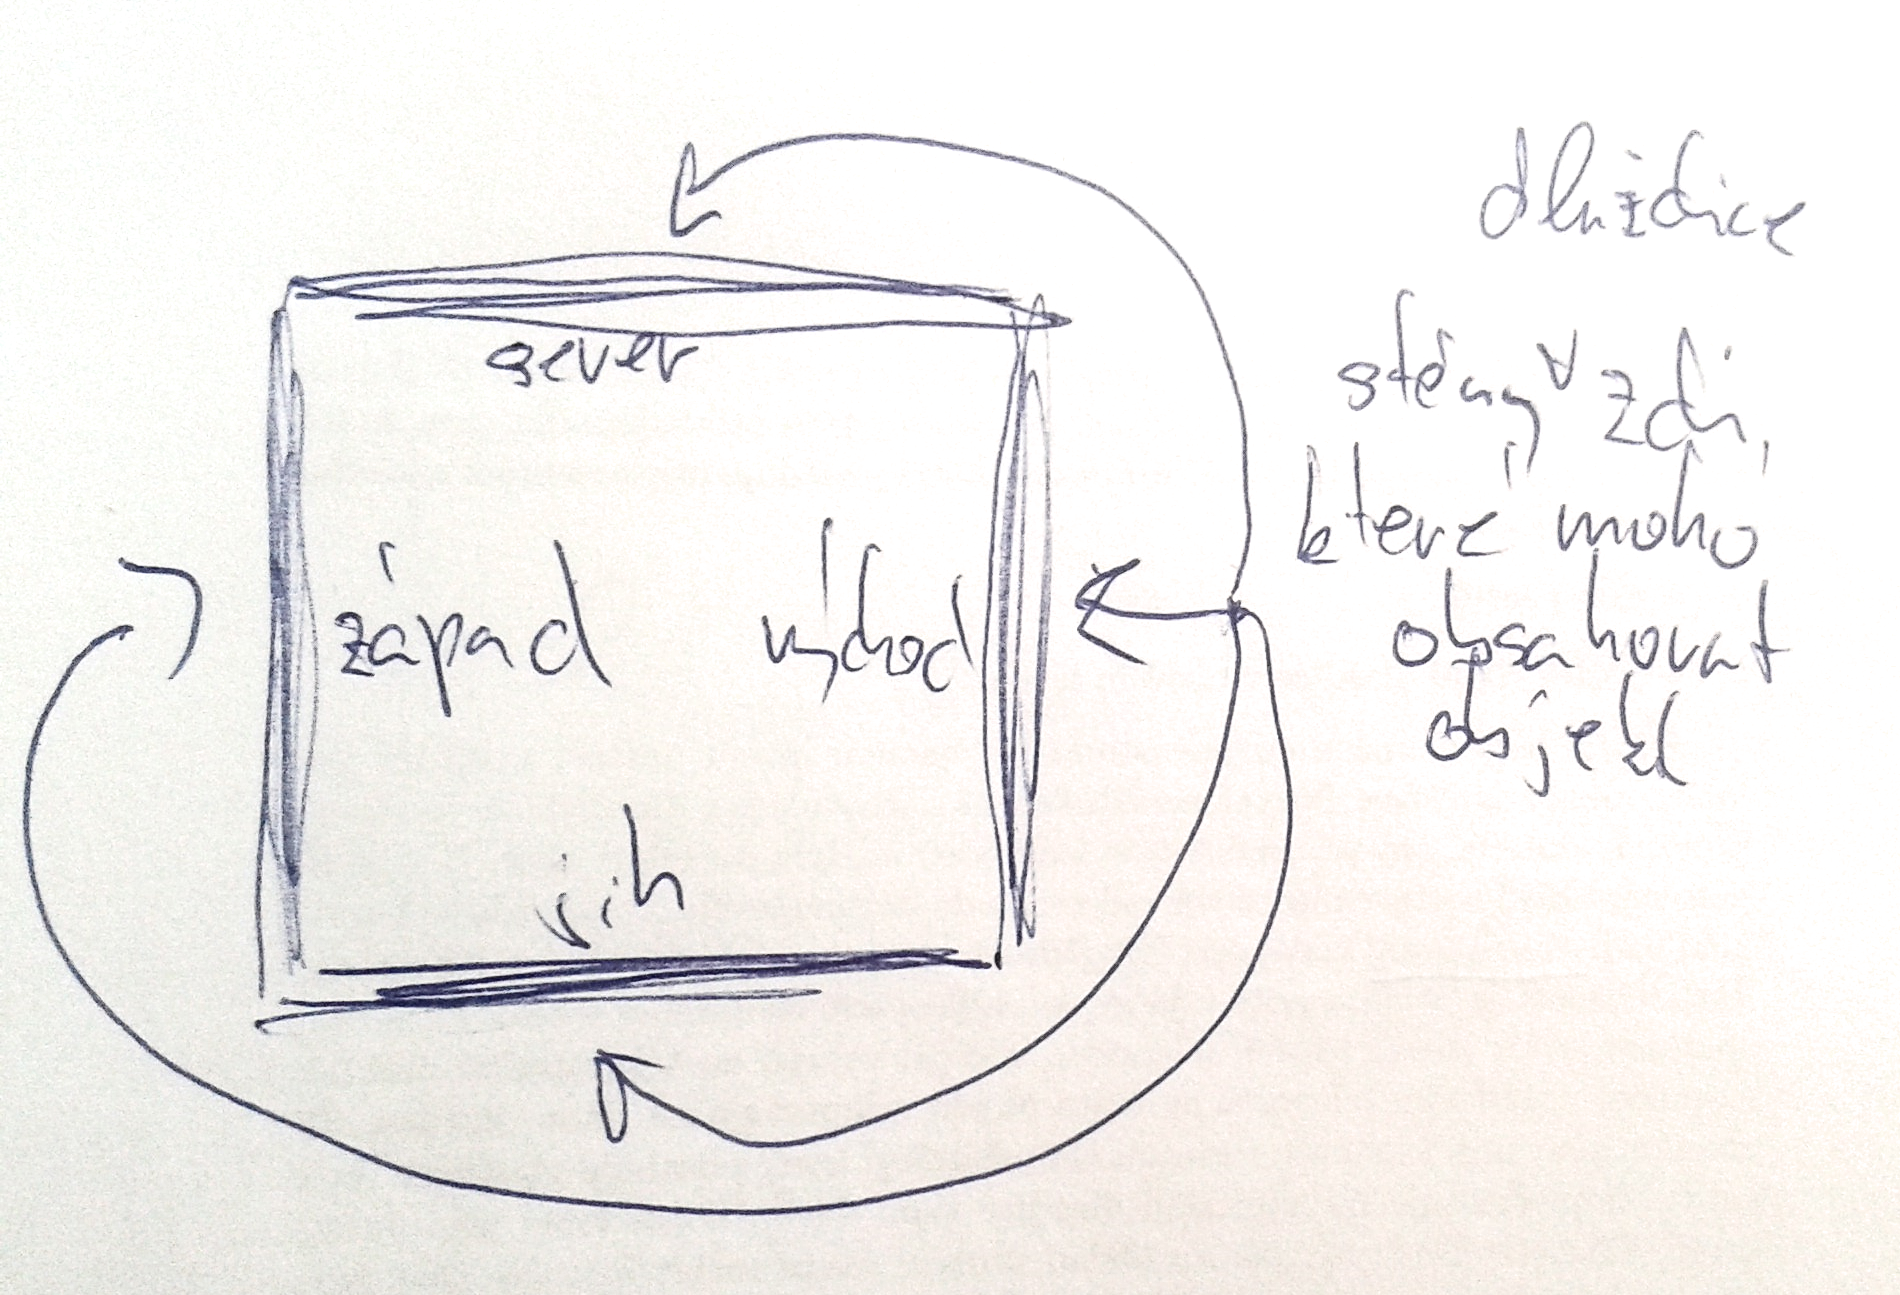
\includegraphics[width=\textwidth]{./img/DM-wall-sides.png}
        \caption{Dlaždice zeď - stěny.}
        \label{wall:analyza}
    \end{subfigure}
    ~ %add desired spacing between images, e. g. ~, \quad, \qquad, \hfill etc. 
    %(or a blank line to force the subfigure onto a new line)
    \begin{subfigure}[b]{0.45\textwidth}
        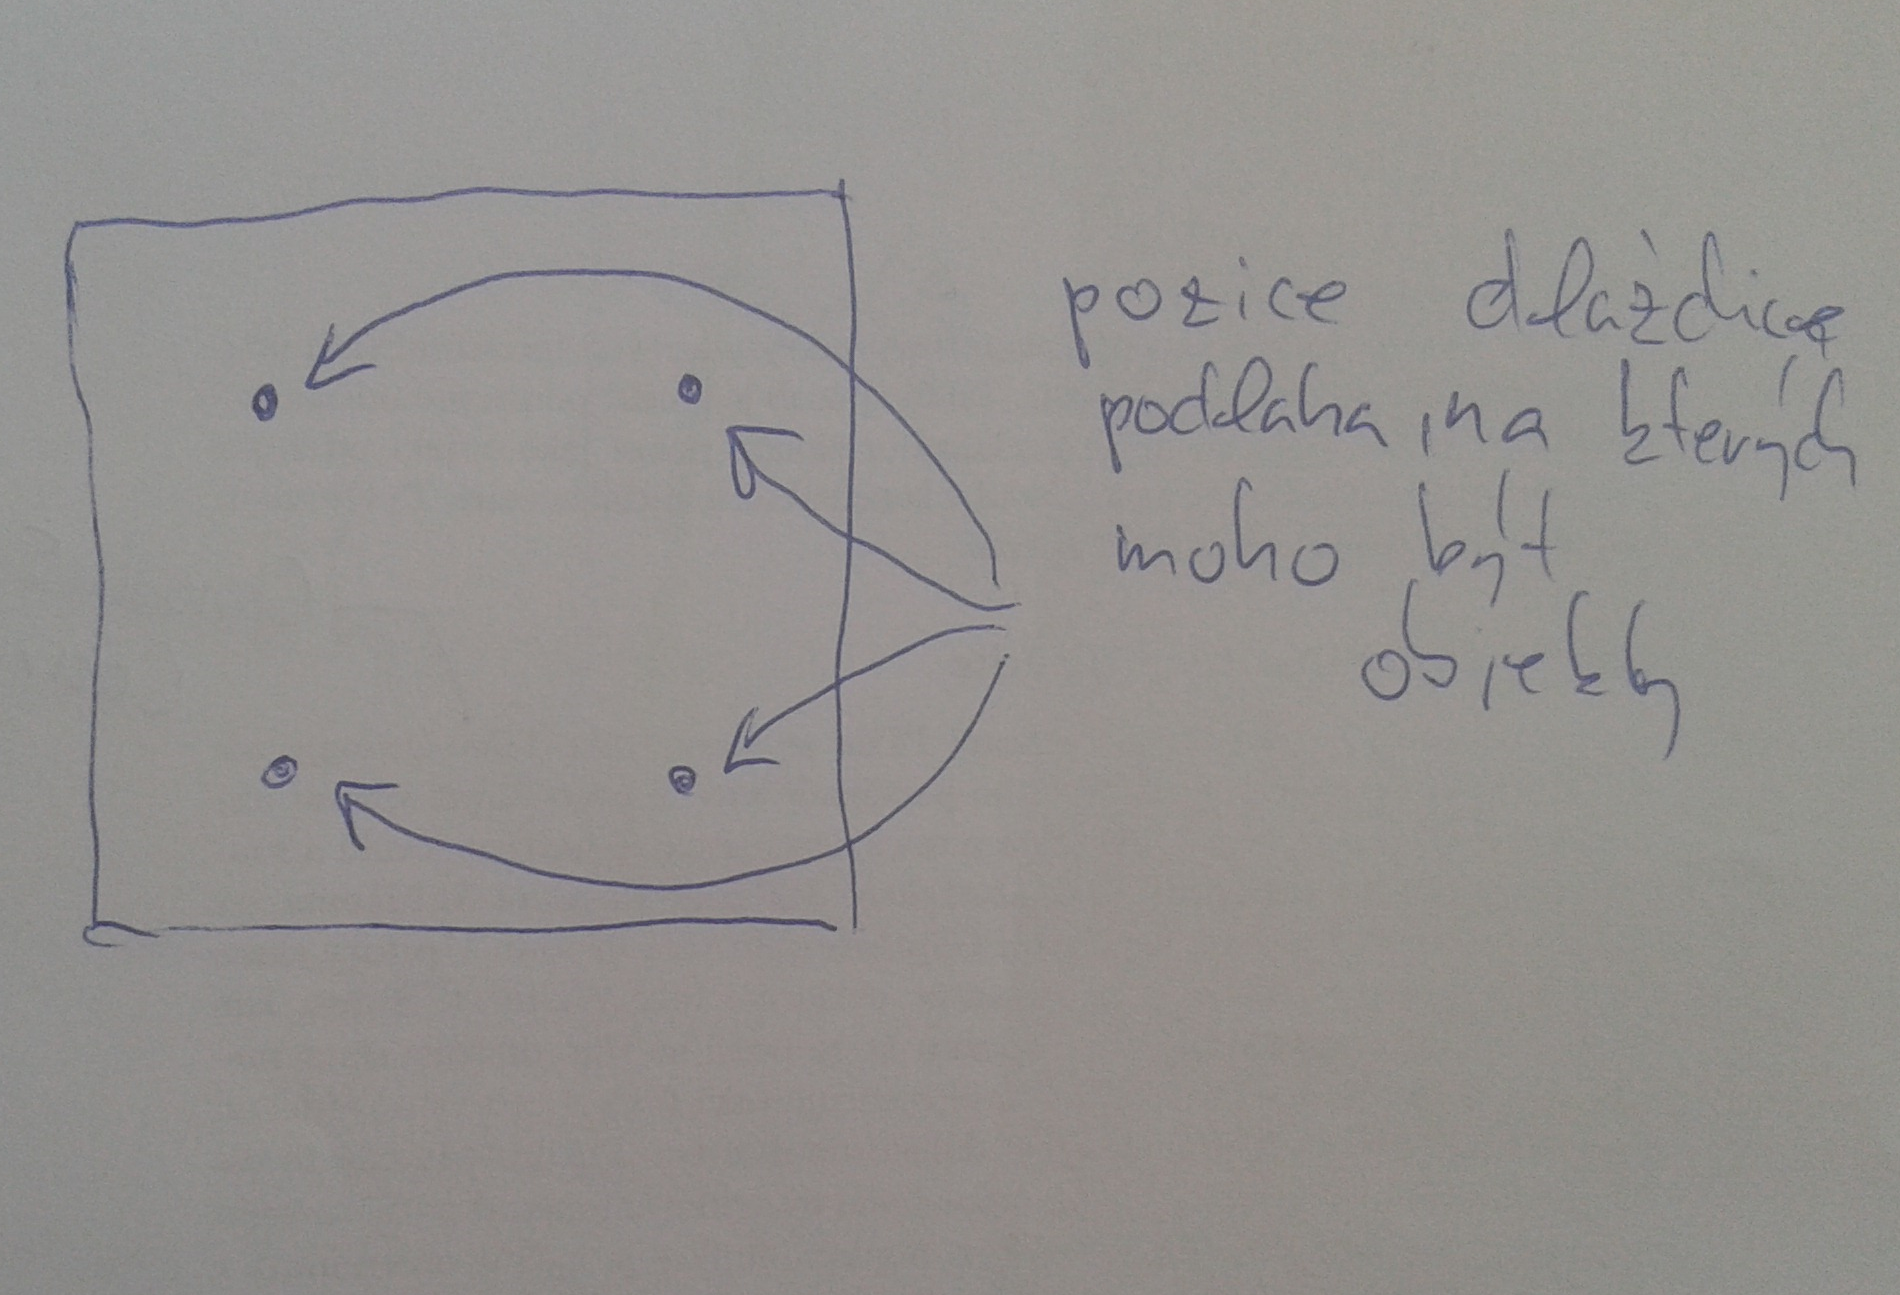
\includegraphics[width=\textwidth]{./img/DM-floor-spaces.png}
        \caption{Dlaždice podlaha - pozice.}
        \label{floor:analyza}
    \end{subfigure}
    \caption{Možné pozice pro uložení objektů na dlaždici.}\label{tile-positions:analyza}
\end{figure}

\begin{figure}[H]\centering
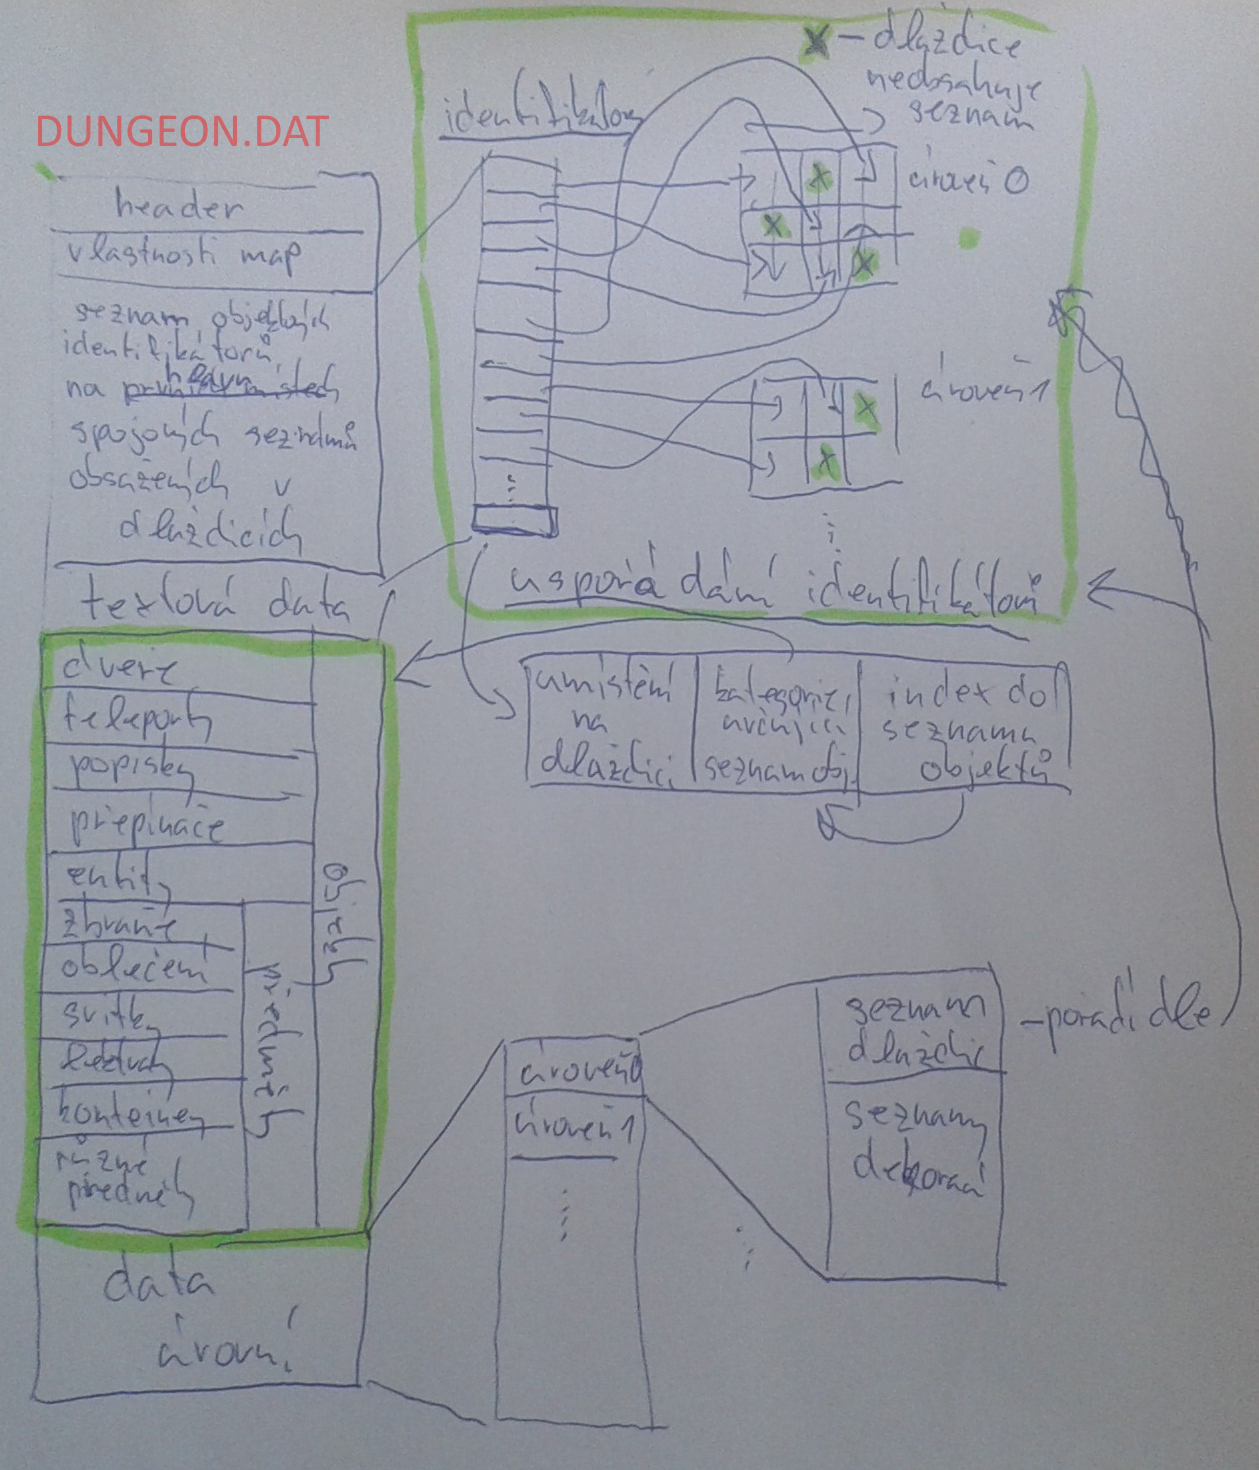
\includegraphics[width=\textwidth]{./img/DM-dungeon-dat.png}
\caption{Ilustrace formátu souboru DUNGEON.DAT}
\label{DM-dungeon-dat:analyza}
\end{figure}

V binárním souboru jsou často data uložena po slovech procesoru, které v tomto případě mají velikost dvou bajtů. 
V další části souboru jsou uložena data s použitými texty ve hře. Tyto texty používají speciální kódování,
kdy jednotlivé znaky jsou uloženy do slov(těch procesorových) a každé toto slovo obsahuje tři znaky. Všechny 
texty jsou pak uloženy za sebou v jednom bloku a ke konkrétním textům je přistupováno přes offsety počtu bajtů
od začátku textových dat. Přesný popis může být opět nalezený v dokumentaci\cite{TechnicalDocumentationFontanel05}.

Kromě sbíratelných předmětů obsahují data ještě další objekty. Řadí se sem dveře, 
teleport, nepřátelské entity, textové popisky a senzory(přepínače). Tyto objekty si lze představit jako instance typů objektů, 
jejichž vlastnosti jsou definované v souboru GRAPHICS.DAT a vymezují pouze vlastnosti, které mohou být různé pro každou instanci.
Za tímto účelem má každý předmět uložený index typu předmětu v dané kategorii.  

Sbíratelné objekty se dělí do následujících kategorií:\label{grabable-items}
\begin{itemize}
\item zbraně - lze je vložit šampionům do ruky a pak s nimi mohou bojovat,
\item oblečení - lze jím obléknout šampiony, a tak zvýšit jejich odolnost,
\item svitky - obsahují text, který může hráči usnadnit hru, 
\item lektvary - dělí se na lektvary modifikující šampionovi schopnosti a na lektvary provádějící nějaké
	akce - např.: výbuch. Každá instance má vlastnost určující sílu efektu.
\item kontejnery - mohou obsahovat další předměty,
\item různé - v této kategorii je například jídlo a pak různé předměty, s kterými nelze provádět žádné akce.
\end{itemize}


Objekt dveře může být pouze na dlaždici typu dveře a obsahuje informace, zda-li jsou dveře rozbitelné a jestli 
mají tlačítko, kterým je lze otevřít. Teleporty mohou být pouze na dlaždici typu teleport a 
definují cílovou dlaždici a kategorii objektů, které teleportují. Textové popisky mohou být pouze na 
dlaždici typu zeď a obsahují odkaz na konkrétní text. Nepřátelské entity jsou definovány po skupinách a určují 
typ příšer ve skupině, jejich počet a využití prostoru na dlaždici. Posledními objekty jsou senzory, 
které vytvářejí základní herní mechaniky bludiště. Senzory mají daný číselný typ, pomocí kterého hra 
určí jakým způsobem je možné senzor
aktivovat. Po aktivaci senzor buď může provést lokální akci nebo odeslat zprávu s akcí na vzdálenou 
dlaždici. Přepínače se pak typicky skládají z několika senzorů. Více o přepínačích a senzorech bude zmíněno
v sekci \ref{actuator-analyza}. 

Ke každému objektu popsanému v předchozích dvou odstavcích existuje unikátní identifikátor\cc{DM-dungeon-dat:analyza}. 
Tento identifikátor se skládá z pozice, která lze buď interpretovat jako světová strana nebo 
umístění na dlaždici - jedná-li se o podlahu. Dále obsahuje kategorii, v které je objekt
uložen. Pro každou kategorii existuje
v datovém souboru seznam instancí objektů dané kategorie. Poslední složkou identifikátoru 
je index do seznamu v dané kategorii. Tyto identifikátory se dají chápat jako reference 
na konkrétní instance objektů.

Každá dlaždice specifikuje, zda může obsahovat spojový seznam složený z objektů zmíněných v předchozích odstavcích. 
Objekty se na sebe potom odkazují pomocí identifikátorů. Další částí datového souboru je pak 
seznam prvních identifikátoru na dlaždicích. Tento seznam obsahuje první identifikátory pro dlaždice
ve všech úrovních. Je seřazen od nejnižší úrovně po nejvyšší od první dlaždice po poslední - bráno  
v každé úrovni po sloupcích.

Samotné úrovně jsou pak vždy definovány následujícími seznamy v tomto pořadí:
\begin{itemize}
\item seznam dlaždic - seřazeny po sloupcích dané úrovně,
\item seznam dekorací příšer,
\item seznam dekorací zdí, 
\item seznam dekorací podlah.
\end{itemize}
Počty jednotlivých dekorací a dlaždic jsou popsány ve vlastnostech úrovní.

\section{Data s vlastnostmi objektů }\label{dungeon-properties}

Soubor GRAPHICS.DAT obsahuje textury dekorací, vlastnosti předmětů a objektů, definici akcí a kouzel.
Formát tohoto souboru nebyl tvůrci uveřejněn, avšak komunitě se opět podařilo data
vyextrahovat i z tohoto souboru. K některým částem také existuje dokumentace\cite{DMGraphicsDAT}, 
nicméně už není tak přehledná a ucelená jako v případě dokumentace pro soubor DUNGEON.DAT. Zároveň 
jsou vyextrahovaná data zveřejněna na webu v HTML formátu. Z toho důvodů jsme se rozhodli 
pro využití již extrahovaných dat v HTML formátu. Dále následuje podrobnější popis využitého obsahu souboru.

\subsection{Akce a komba}\label{action-combos}

S předměty je možné provádět akce. Množina akcí pro daný předmět se nazývá kombo a obsahuje 
až tři akce. Ve hře je k dispozici čtyřicet čtyři akcí a stejný počet komb. Kompletní seznam jednotlivých
akcí a komb viz\cite{DMActions}. Zde popišme alespoň jejich vlastnosti.

Vlastnosti akcí jsou :
\begin{itemize}
\item název 
\item zkušenosti - počet zkušeností získaných po provedení akce,
\item dovednost - identifikátor dovednosti, která získá zkušenosti,
\item obrana - modifikátor obrany při používání akce,
\item výdrž - modifikátor výdrže nutné pro provedení akce, 
\item pravděpodobnost provedení akce 
\item zranění - modifikátor pro výpočet konečného zranění nepřítele, 
\item únava - doba po kterou nelze provádět žádné akce. 
\end{itemize}

Vlastnosti pro každou akci komba jsou:
\begin{itemize}
\item index akce ze seznamu akcí, 
\item úroveň dovednosti - minimální úroveň dovednosti pro úspěšné provedení akce. 
\end{itemize}


\subsection{Předměty}\label{item-descriptors}

Ke každému typu předmětu existují v tomto souboru popisovače vlastností\cite{DMItemDescriptors}.
Pro každý předmět jsou definovány následující vlastnosti:  
\begin{itemize}
\item globální identifikátor - unikátní identifikátor, který je použit k identifikaci konkrétního typu předmětu například v přepínačích,
\item index útočného komba,
\item lokace - místo, na kterou část těla nebo, do kterého inventáře šampiona lze předmět vložit,
\item index v kategorii - index typu předmětu v dané kategorii.
\end{itemize}

Globální identifikátor lze z instance předmětu získat pomocí jeho kategorie a indexu typu předmětu,
který má každá instance předmětu. Každý předmět má také definovanou hmotnost. Zbraně a oblečení mají navíc
definované následující vlastnosti\cite{DMItems}.

Zbraně:
\begin{itemize}
\item poškození - hodnota zranění aplikována při útoku na nepřítele,
\item kinetická energie - hodnota udává, jak daleko lze zbraň hodit,
\item střelné poškození - hodnota dodatečného poškození u střelných zbraní.
\end{itemize}

Oblečení:
\begin{itemize}
\item síla brnění - obrana, kterou oblečení poskytuje, 
\item odolnost proti útoky ostrými předměty. 
\end{itemize}

\subsection{Kouzla a symboly}\label{magic-symbols}

Další častí dat uložené v souboru GRAPHICS.DAT jsou vlastnosti kouzel. Pojďme si nejprve přiblížit,
jak se ve hře kouzla přesně vyvolávají. Každé kouzlo je složeno z několika symbolů, přičemž první 
z nich je speciální a jde o tzv. ,,power symbol". Power symbol určuje, jak bude celkové kouzlo silné.
Další symboly už určují konkrétní kouzlo. Každé vyvolání symbolu stojí šampiona manu. Po stanovení 
všech symbolů může šampion vyvolat samotné kouzlo. Vyvolání kouzla může selhat, pokud nemá šampion 
dostatečnou úroveň dovednosti vyžadované kouzlem. Datový soubor tedy obsahuje pro každý symbol při odpovídajícím
power symbolu množství potřebné many pro jeho vyvolání. Dále obsahuje následující vlastnosti kouzel\cite{DMSpells}:

\begin{itemize}
\item modifikátor obtížnosti,
\item dobu - po které šampion nemůže vyvolávat další kouzla,
\item úroveň dovednosti - nutné pro vyvolání kouzla.
\end{itemize}

\subsection{Nepřátelské entity}\label{properties-creatures}

Poslední částí obsaženou v souboru GRAPHICS.DAT, kterou jsme využili, jsou vlastnosti nepřátelských entit.
Následující výčet obsahuje vlastnosti, které implementuje nový engine. 
\begin{itemize}
\item doba mezi pohybem 
\item doba mezi útoky
\item síla brnění
\item zdraví
\item síla útoku
\item otrava - určuje, zda útok může způsobit otravu
\item obrana 
\item dohled 
\item vzdálenost, na kterou detekuje nepřítele bez vidění 
\item odolnost proti ohni
\item odolnost proti jedu
\item pravděpodobnosti zranění určitých částí těla
\end{itemize}

Celý seznam vlastností je možné nalézt v dokumentaci\cite{DMCreatures}.


\section{Parsování vstupních dat}\label{level-parsing}

V době implementace této části práce nebylo jasné, zda nalezená dokumentace\cite{TechnicalDocumentationFontanel05} bude dostatečná
pro splnění práce. Parser je proto oddělen od zbytku enginu do zvláštní assembly, která nereferencuje žádnou knihovnu
pro zobrazování grafiky. Cílem této assembly je tedy pouze převést struktury obsažené ve vstupních datech do odpovídajících
datových tříd v jazyce C\#. Tento balík dat se potom předá enginu, který z něj nich vytvoří herní úrovně. Toto schéma 
znázorňuje následující obrázek \ref{parser-preview:analyza}.

\begin{figure}[H]\centering
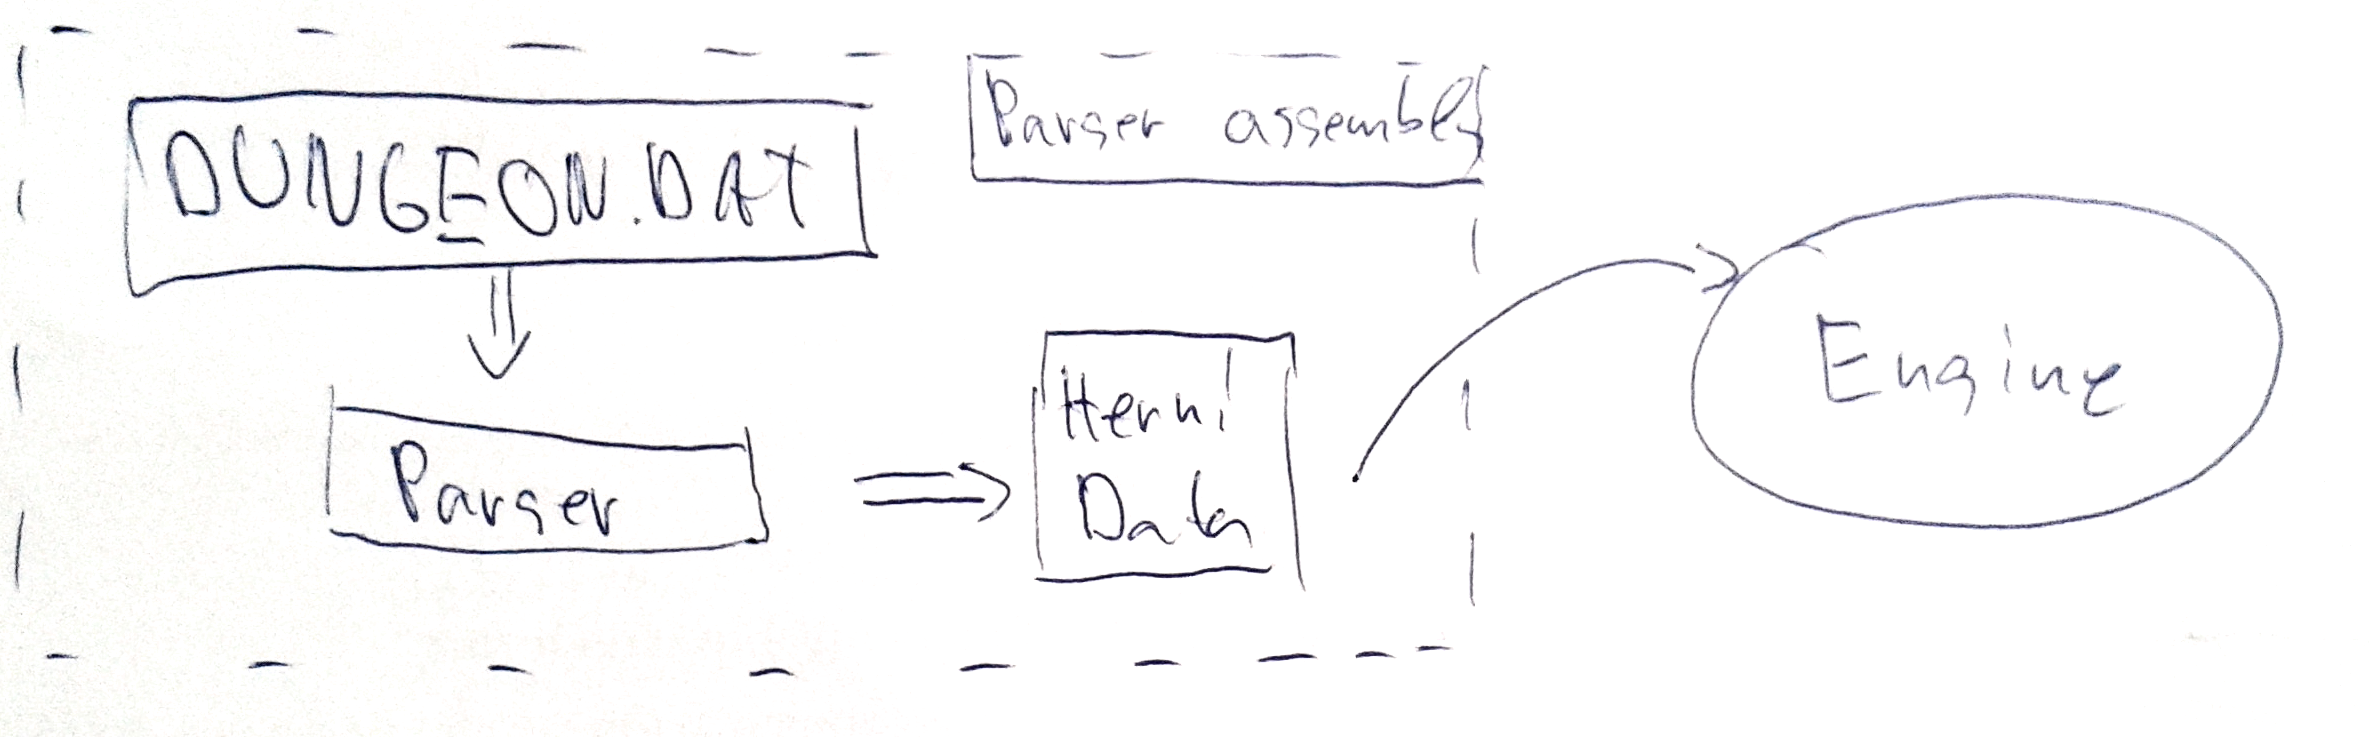
\includegraphics[width=\textwidth]{./img/DM-parser-preview.png}
\caption{Ilustrace vztahu parseru k enginu.}
\label{parser-preview:analyza}
\end{figure}

\subsection{Herní úrovně - DUNGEON.DAT}\label{dungeon-parser}

Parsování herních úrovní je rozděleno do dvou fází. V první fázi probíhá transformace dat objektů\vref{dungeon-objects} ze souboru DUNGEON.DAT
 na odpovídající objekty v jazyce C\#. V druhé fázi jsou pak objekty z první fáze upraveny,
aby měli přehlednější strukturu. 


\subsubsection{První fáze}

V této fázi je nejprve vytvořen datový objekt, který bude shromažďovat všechny ostatní data. Tento objekt obsahuje:

\begin{itemize}
\item metadata z hlavičky souboru - to jsou zejména velikosti všech seznamů s objekty\vref{dungeon-objects} a počet map,
\item seznamy objektů - to jsou seznamy objektů jazyka C\# vzniklé rozparsováním odpovídajících dat objektů v souboru,
\item seznam herních úrovní - to jsou objekty reprezentující data herních úrovní, které obsahují jejich vlastnosti\vref{dungeon-objects}
 a seznam jejich dlaždic, dekorací, atd. 
\end{itemize}

Dále parser rozparsuje všechny data vstupního souboru dle dokumentace\cite{TechnicalDocumentationFontanel05} a vytvoří z nich 
adekvátní objekty, které uloží do zmíněného datového objektu. Ilustrace této fáze je na obrázku \ref{dungeon-parser}.

\subsubsection{Druhá fáze}
Po skončení první fáze je struktura vzniklého datového objektu podobná struktuře souboru DUNGEON.DAT. Tím máme namysli, že
například spojové seznamy jsou reprezentovány pomocí objektových identifikátorů\vref{dungeon-objects}, což není příliš intuitivní a pro práci 
s těmito daty by engine musel rozumět jejich formátu. Navíc spojové seznamy obsahují objekty různých typů. Proto pro zjednodušení práce enginu
s těmito daty jsou v datových objektech inicializovány ještě následující položky: 
\begin{itemize} 
\item seznam sbíratelných předmětů,
\item seznam senzorů,
\item seznam popisků,
\item seznam nepřátelských entit,
\item položku dveří pro dlaždici typu dveře,
\item položku teleport pro dlaždici typu teleport,
\item a pro dlaždici typu zeď a podlaha stanoví identifikátory náhodných dekorací.
\end{itemize} 

Na počátku vývoje projekt neobsahoval druhou fázi, její vytvoření vedlo k zjednodušení kódu v enginu.

\subsection{Vlastnosti objektů - GRAPHICS.DAT}

Pro sestavení herních úrovní potřebuje engine také vlastnosti společné pro všechny konkrétní typy objektů ze
souboru DUNGEON.DAT. Jak bylo zmíněno v sekci \ref{dungeon-properties}, tyto vlastnosti jsou v originální hře v souboru GRAPHICS.DAT.
Nicméně tato data již existují vyextrahovaná v HTML formátu, a proto jsme je použili namísto původních dat.
Ke zjednodušení parsování dat z HTML souborů byla
použita knihovna HTML Agility Pack\cite{HtmlAgilityPack}. Pro každé typy vlastností jsou pak vytvořeny odpovídající datové objekty
které jsou uloženy do seznamů ve výsledném datovém objektu zmíněného v předchozí
sekci\ref{dungeon-parser}. V této části jsou získána data vlastností všech objektů\vref{dungeon-objects} až na kouzla.
Vlastnosti kouzel jsou rozparsovány v enginu přímo do objektů v něm použitých. Proto by případné vytváření datových souborů
v této vrstvě bylo zbytečné. Celý proces zobrazuje diagram na obrázku \ref{parser:analyza}.

\begin{figure}[H]\centering
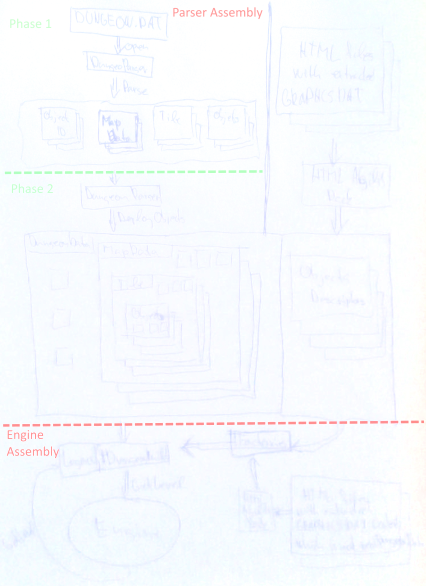
\includegraphics[width=\textwidth]{./img/DM-parser.png}
\caption{Průběh parsování herních dat.}
\label{parser:analyza}
\end{figure}

\section{Výběr frameworku pro práci s grafickým výstupem}

Po úspěšném rozparsování herní dat se bylo třeba rozhodnout, kterou knihovnou použít pro zobrazení grafického výstupu enginu. 
Cílem této práce je vytvořit herní engine s dobrým návrhem\aref{aim-extensibility}. Proto stačí, aby byl grafický výstup ve formě proof of concept. 
Aby se bylo možné soustředit hlavně na samotný návrh enginu, použili jsme framework, s který už jsme měli nějaké zkušenosti.
Jedná se o XNA Framework od firmy Microsoft. Nicméně tento framework již není firmou nadále podporován a vyvíjen, proto jsme využili 
konečně jeho klon MonoGame\cite{MonoGame}. Výhodou této volby je také to, že framework je multiplatformní. Jeho tvůrci tvrdí, že podporuje platformy
iOS, Android, MacOS, Linux, Windows , OUYA, PS4, PSVita, Xbox One.

\section{Reprezentace jádra enginu}\label{engine-core-section}

O samotnou herní smyčku se stará framework MonoGame, který na jádru enginu volá aktualizační a vykreslovaní obsluhy\cc{engine-core}.
Jádro enginu pak obsahuje následující tři důležité komponenty:
\begin{itemize}
\item Hráč - tato komponenta zajišťuje interakci s uživatelem. Skrze ni lze ovládat hráčovu skupinu šampionů, sbírat předměty nebo bojovat.
\item Builder herních úrovní - tato komponenta zajišťuje sestavování herních úrovní.
\item Objekt obsahující továrny na herní objekty - pro každý typ popsaný v sekci \ref{dungeon-properties} existuje odpovídající
	továrna obsahující jeho vlastnosti. Továrny pak mohou vytvářet objekty, jejichž typ reprezentují. Toto bude konkrétně
	specifikováno později\vref{item-factories}, nicméně důležité je, že skrze jádro enginu lze k těmto továrnám přistupovat.
\end{itemize}
Konkrétní implementace předchozích komponent lze do jádra enginu vložit při jeho inicializaci. Tímto způsobem může být herní 
engine rozšířen o nové funkce. Následující funkce enginu jsou znázorněny na obrázku \ref{engine-core}.

Prvním úkolem jádra enginu je starat se ve správný moment o načítání a propojování herních úrovní. Pro splnění této funkce
obsahuje jádro kolekci právě používaných úrovní. Tato kolekce si pamatuje vždy tři poslední načtené úrovně.
Při každé změně aktuální dlaždice hráče se vyhledají dlaždice v jeho viditelném dosahu, který je určen podle výše aktuálního osvětlení.
Pokud některá z těchto dlaždic vede do jiné úrovně, pak je tato úroveň načtena pomocí builderu. Samotné objekty reprezentující herní úrovně 
obsahují pouze seznam dlaždic, číslo úrovně, obtížnost úrovně a umožňují vyhledat dlaždici dle její pozice. 

Jádro se také stará o vykreslování všech objektů. Každá dlaždice má u sebe uložený seznam objektů, které požadují vykreslování.
Je na samotných objektech, aby se do kolekcí na odpovídajících dlaždicích přehlašovaly resp. odhlašovaly. Jádro pak při 
cyklu vykreslování projde všechny viditelné dlaždice a vykreslí jejich objekty. Hráčovy objekty jsou vykreslovány skrze komponentu hráče.

Některé objekty také potřebují aktualizovat svůj stav. Takové objekty se pak musí zaregistrovat do kolekce v herní úrovni,
do které náleží. V každém cyklu herní smyčky se potom projdou všechny aktivní úrovně a aktualizují se objekty v jejich kolekci.
Hráč je opět aktualizován přímo skrze komponentu hráče.

Posledním úkolem jádra je aktualizovat osvětlení. Osvětlení je aktualizované v každým cyklu herní smyčky. Úroveň osvětlení 
se pak vypočítá na základě světelných zdrojů, které mají šampioni v hráčově skupině.

\begin{figure}[H]\centering
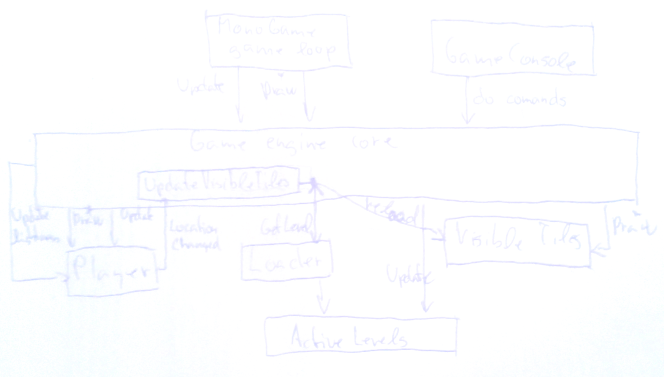
\includegraphics[width=\textwidth]{./img/engine-core.png}
\caption{Ilustrace funkce jádra enginu.}
\label{engine-core}
\end{figure}


\section{Reprezentace dlaždic}\label{tile-representation}

V originální hře jsou dlaždice vždy uloženy v obdélníkovém poli\vref{dungeon-objects}. To znamená, že dlaždice, které nejsou využity pro~chodby,
jsou vždy vyplněny zdmi. Jelikož jedním z cílů této práce je udělat engine co nejrozšiřitelnější\aref{aim-extensibility}, rozhodli jsme se tento problém vyřešit
o něco obecněji. Mezi dlaždicemi jsou vazby, které s nimi dohromady tvoří obousměrný orientovaný graf. Nicméně, pro dlaždice stále platí, že musí být
uspořádané do mřížky. Každá z dlaždic má potom stále nejvýše čtyři sousedy. Tato reprezentace pro hodně řídké mapy může ušetřit paměť.
Avšak důležitější je, že při takové reprezentaci lze jednoduše získat sousedy pouze ze znalosti konkrétní dlaždice. V této 
podobě by bylo navíc jednoduší engine upravit tak, aby dlaždice nemusely být na mřížce a aby mohli mít více sousedů.

Předchozí rozhodnutí také vede k tomu, že již nejsou potřeba dlaždice typu zeď\cc{tile-representation-img}, jelikož její stěny můžou být definovány ve 
dlaždicích typu podlaha. Při vytváření podlahy je pak nutné číst i její sousední dlaždice. Pokud je soused daným směrem zeď, 
vytvoří se na této straně stěna a soused není nastaven. V opačném případě je soused nastaven na odpovídající dlaždici.
Zprávy původně cílené zdím je také třeba posílat na odpovídající dlaždice podlahy. Tato reprezentace zdí opět vede k
vyšší flexibilitě, jelikož případné místo využité původními dlaždicemi typu zdi lze využít jiným způsobem.

\begin{figure}[H]\centering
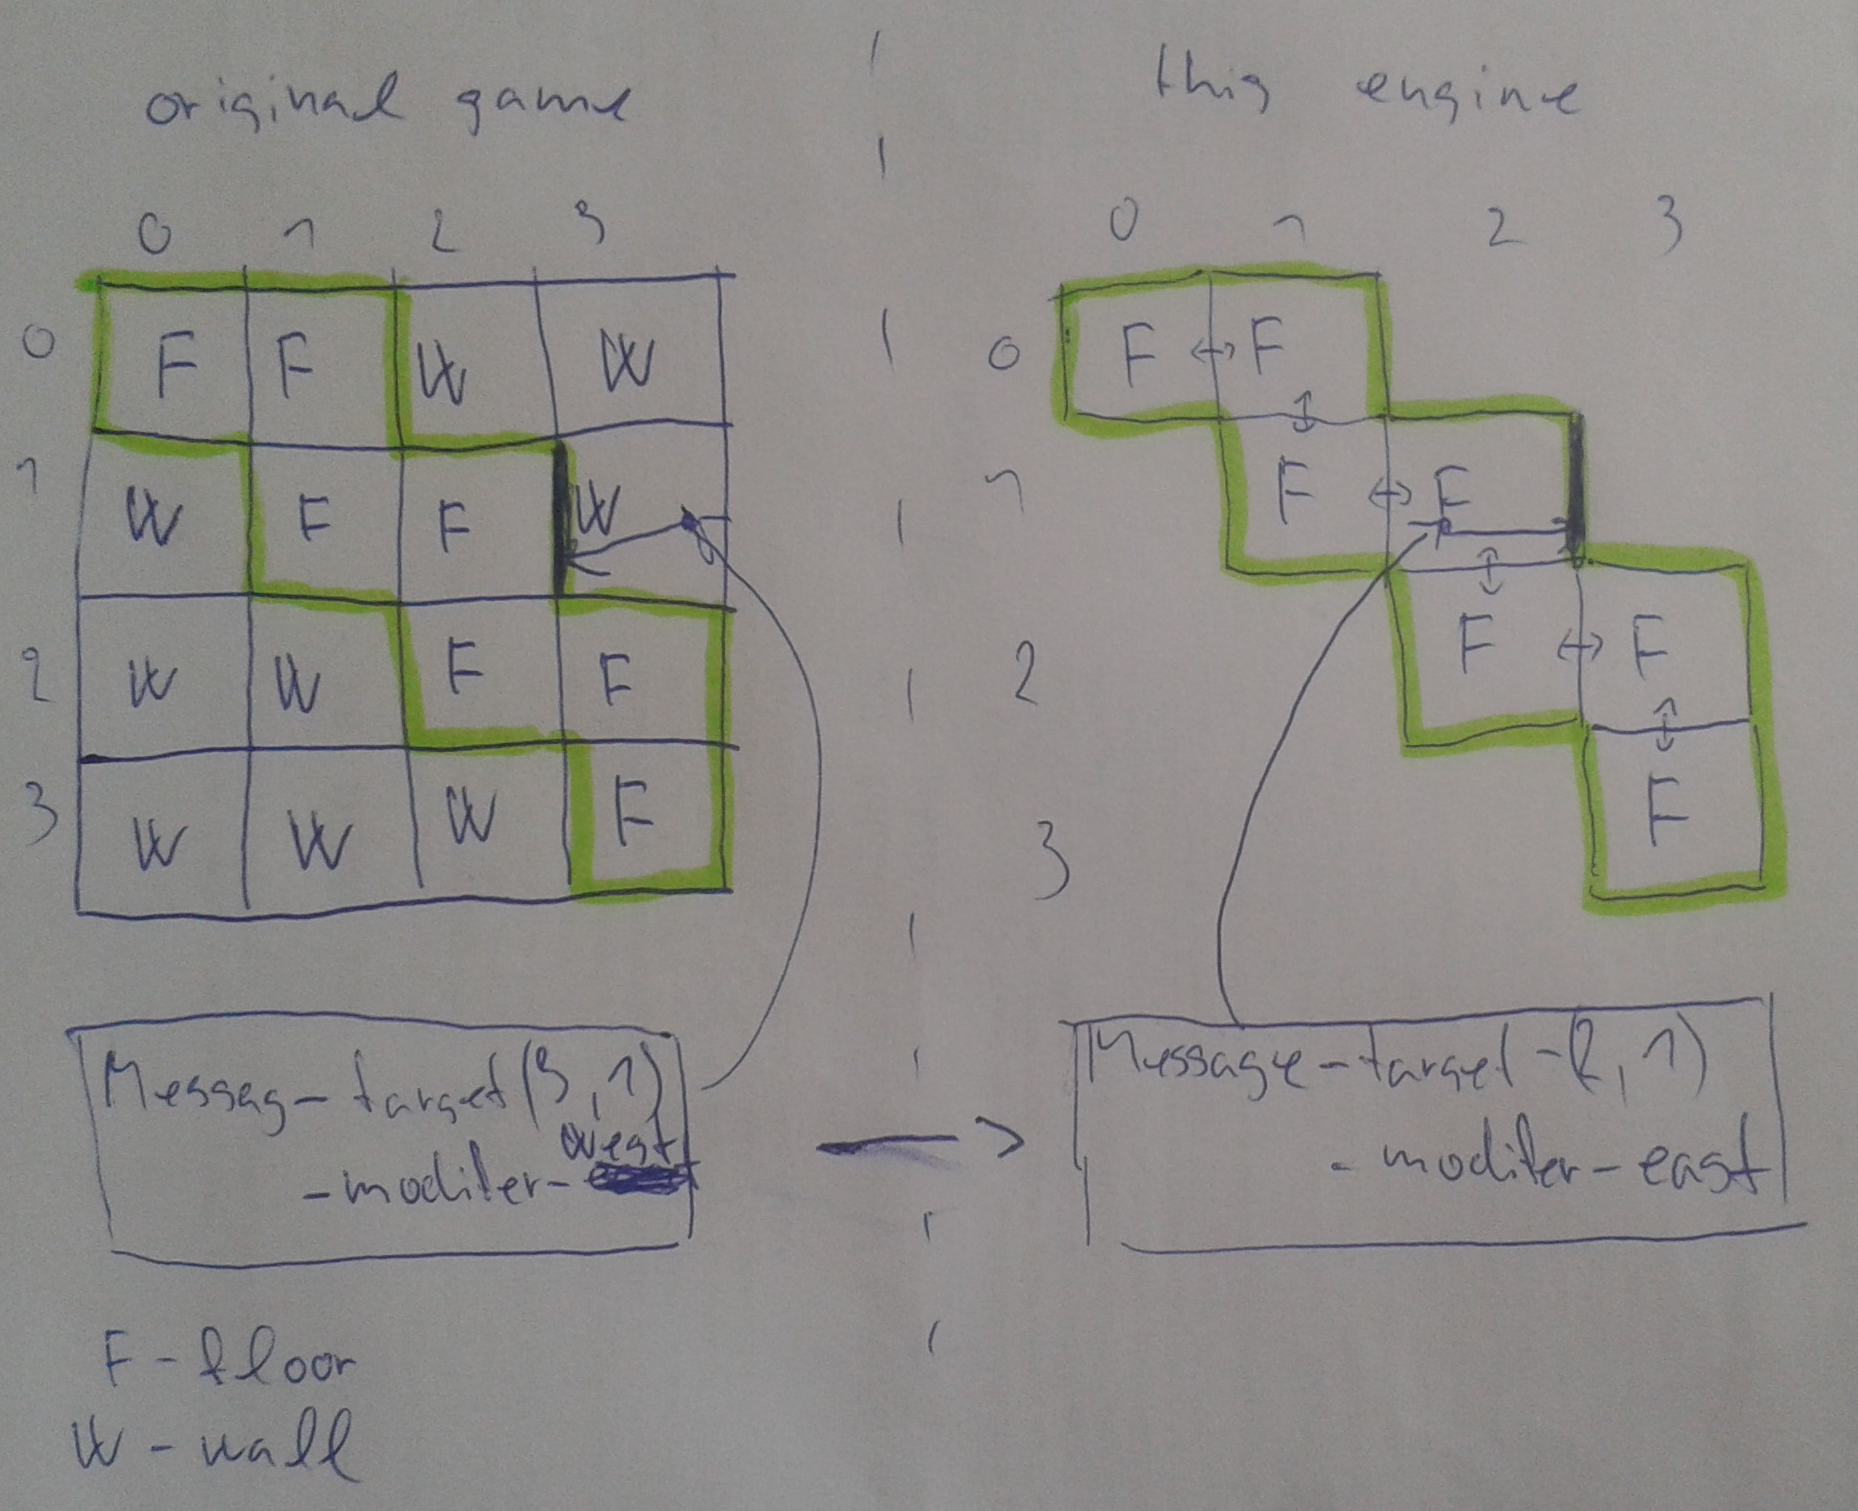
\includegraphics[width=\textwidth]{./img/tile-representation.png}
\caption{Uložení dlaždic v originálním vs tomto enginu.}
\label{tile-representation-img}
\end{figure}

Pokud jsou tedy stěny součástí dlaždic, je třeba vyřešit jejich reprezentaci. Buď je možné, aby veškeré funkce stěn obsahovala přímo
dlaždice, a nebo je možné tyto části delegovat do zvláštních objektů. Ze začátku byl v enginu použit první zmiňovaný způsob. Nicméně 
tato reprezentace není příliš vhodná, protože potom samotná dlaždice řeší funkce, které k ní přímo nenáleží.
Nakonec tato reprezentace byla změněna a v enginu byla použita druha zmiňovaná možnost. Vedlo k ní zejména oddělení zobrazovací vrstvy 
od logické. Výhoda tohoto přístupu byla kromě samotného oddělení kódu i možnost znovu použití kódu za pomocí dědičnosti. 
Například třída reprezentující stěnu, která obsahuje přepínač, může dědit ze třídy reprezentující prázdné stěny. 
Avšak ukázala se i nevýhoda tohoto přístupu, a to, že komunikace směrem ze stěny k dlaždici je trochu těžkopádná.
Buď by bylo zapotřebí předat zdi referenci na jejich rodičovské dlaždice, nebo by se museli
použít události. Pokud to bylo v některých případech nutné, přiklonili jsem se k použití událostí.

\section{Přepínače}\label{actuator-analyza}
Přepínače tvoří základní mechaniky v herních úrovních Dungeon Masteru, mohou být buď na stěnách, nebo na podlaze. 
Na stěnách je lze aktivovat kliknutím myši a na podlaze potom přesunutím hráče na dlaždici s přepínačem. Aktivace ještě
může být podmíněna dalšími faktory: obsah daného typu předmětu v ruce nebo směr kterým je hráč otočen.  

Ve skutečnosti se každý přepínač skládá z řady senzorů a platí, že:
\begin{itemize}
\item poslední senzor určuje dekoraci přepínače,
\item při pokusu o aktivaci přepínače, dojde postupně k pokusu aktivace každého senzoru,
\item každý senzor může definovat akci, kterou provede, pokud byl aktivován.
\end{itemize}

Senzor má následující vlastnost:
\begin{itemize}
\item Typ - číselné označení, dle kterého originální herní engine určí způsob aktivace.
\item Akce - může být buď lokální, nebo vzdálená. Pro lokální akce je to zarotování sekvencí senzorů 
	přepínače\cc{actuator-rotation} nebo přidání zkušeností hráči. Pro vzdálené akce je to odeslání zprávy\vref{dungeon-objects} na danou cílovou dlaždici. 
\item Data pro lokální resp. vzdálenou akci.
\item Zpoždění - doba, po které se provede akce.
\item Opačný efekt - liší se dle typu senzoru, nicméně většinou otáčí podmínku aktivace pro daný typ senzoru. 
\item Opakovatelnost - určuje, zda lze senzor aktivovat neomezeně krát či pouze jednou.
\item Dekorace  
\end{itemize}

\begin{figure}[H]\centering
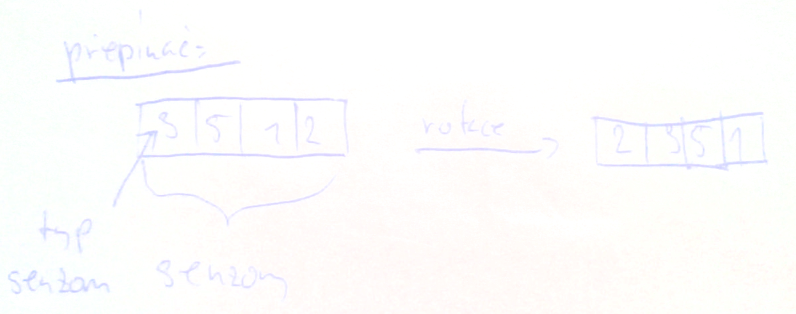
\includegraphics[width=\textwidth]{./img/actuator-rotation.png}
\caption{Ilustrace rotace sekvence senzorů.}
\label{actuator-rotation}
\end{figure}


Výše popsaný systém přepínačů přináší hned několik problémů:
\begin{enumerate}
\item\label{actuator-unclear} Z technické dokumentace\cite{TechnicalDocumentationFontanel05} není vždy jasně zřejmé, jaká je aktivační podmínka senzoru pro určitý typ.
\item\label{actuator-effective} Jakým způsobem efektivně a přehledně rozparsovat data senzorů, když mají tolik nezávislých vlastností.
\item\label{actuator-representation} Jak reprezentovat přepínače v novém enginu.
\item\label{actuator-remote-actions} Jakým způsobem provádět vzdálené akce.
\end{enumerate}

\subsection{Reprezentace přepínačů}
První tři body problémů(viz \ref{actuator-unclear}, \ref{actuator-effective}, \ref{actuator-representation}) řeší tato sekce.

\subsubsection{První reprezentace}\label{rep-v1}

Jako první způsob jsme se rozhodli vždy pro několik sekvencí senzorů vytvořit objekt, který měl stejné nebo o něco obecnější vlastnosti než dané sekvence.
Z počátku se totiž zdálo, že jen výjimečně jsou sekvence senzorů větší či složitější. Proto jsme se rozhodli vytvořit v
novém enginu objekty, které mají obecnější vlastnosti, a tak mohou být použité pro několik podobných sekvencí. Dle určité sekvence senzorů se poté
objektu inicializují jeho vlastnosti. Celou situaci ilustruje obr. \ref{actuator-object}.

\begin{figure}[H]\centering
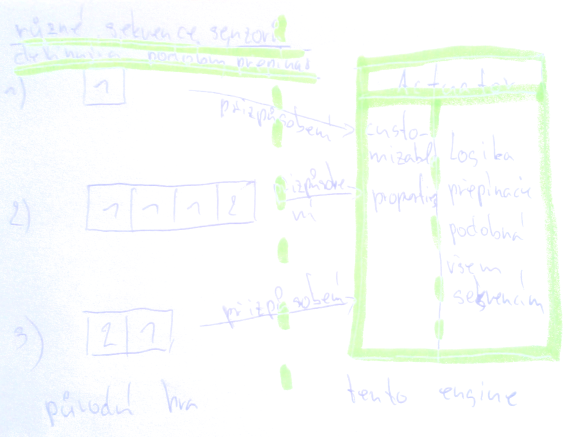
\includegraphics[width=\textwidth]{./img/actuator-object.png}
\caption{Ilustrace transformace sekvence senzorů na objekt přepínač.}
\label{actuator-object}
\end{figure}

Tento způsob sice řeší problém samotné reprezentace\vbref{actuator-representation}, ale později se ukázalo, že velice nevhodně. Například
kód převádějící sekvence na přepínače je složitý a nepřehledný. Bylo také složité vytvořit přepínač podle technické dokumentace\cite{TechnicalDocumentationFontanel05}
tak, aby fungoval správně. Popis v dokumentaci\cite{TechnicalDocumentationFontanel05} také není dostatečně přesný pro vytvoření tohoto úkolu.
I proto čím více přepínačů jsme tímto způsobem naimplmentovali, tím více se ukazovalo problémů. Nakonec jsme dospěli k závěru, že tento způsob reprezentace je nemožný.

\subsubsection{Druhá reprezentace}

Tato reprezentace se snažila vyřešit problém nepřehlednosti kódu\vbref{actuator-effective} převádějícího sekvence na objekty přepínačů.
Proto je i zde použit typ objektu přepínač z první reprezentace v sekci \ref{rep-v1}. Parsování sekvence senzorů jsme se rozhodli udělat pomocí konečného 
automatu. Tedy tak, že pro každý objekt přepínače existovaly předdefinované sekvence senzorů. Konečný automat potom pomocí vstupní sekvence
identifikoval výsledný objekt přepínače. Při inicializaci objektu přepínače zde pak byla sekvence jasně definovaná, což řešilo problém s přehledností \vbref{actuator-effective}.
Později se však ukázalo, že i malá změna v sekvenci senzorů může generovat podobný objekt. Takže by bylo třeba
spoustu předdefinovaných šablon, které by se lišily ve drobnostech. Tím se ukázalo, že tento přístup není dostatečně obecný a nelze jej tedy použít. 

\subsubsection{Třetí reprezentace - výsledná}

Tato reprezentace se oproti předchozím snažila přiblížit co nejvíce k systému použitém v enginu originální hry.
K dosažení tohoto cíle jsme se rozhodli použít dekompilované zdrojové kódy\cite{DMDecompilation} hry. Tím
je vyřešen problém nedostatečné dokumentace ve věci přepínačů\vbref{actuator-unclear}.

Vytvořili jsme tedy objekt přepínač, který má v sobě sekvenci senzorů, tak jako tomu je v originální hře.
Tím je vyřešen i problém nepřehlednosti převodního kódu\vbref{actuator-effective}, jelikož jsou tyto reprezentace téměř identické.
S využitím zdrojových kódů jsme vytvořili odpovídající objektově orientovaný kód v jazyce C\#. Tato reprezentace
tak zajišťuje maximální korektnost implementace a přitom poskytuje možnost rozšíření - což je jedním z cílů této práce(viz bod \ref{aim-extensibility}). 
Je tedy možné vytvořit nové senzory, které budou mít vlastní aktivační podmínky a ty následně použít v přepínačích.
V originálním enginu je toto rozšiřovaní jen značně omezené, jednotlivé typy senzorů se tam odlišují jednobajtovým číselným identifikátorem.
Ale jelikož jsme nechtěli rozšiřování enginu limitovat pouze na tento způsob vytváření senzorů, je možné si vytvořit přepínač, který
bude fungovat na úplně jiné bázi. Takže případné nové přepínače nemusí vůbec senzory používat. 

\subsection{Reprezentace zprávy přepínače}\label{actuator-message-representation}

Jak již bylo řečeno\vref{dungeon-objects}, celý systém mechanik herních úrovní je závislý na posílání zpráv. 
V originální hře je cíl odeslané zprávy vázán na její souřadnice dlaždice. 
Jelikož jsme se v enginu nechtěli vázat na tyto pevné souřadnice, rozhodli jsem se namísto nich
cílovou dlaždici identifikovat její referencí. To by případně ulehčilo práci při transformaci enginu tak, aby
dlaždice mohli mít více sousedů nebo aby nemusely být na pevné mřížce\vref{tile-representation}.
Při takovéto reprezentaci však nastává problém s inicializací dlaždic a přepínačů\vref{level-inicialization}.

V originální hře lze mezi dlaždicemi posílat pouze jeden typ zprávy. Jelikož cílem této práce je udělat engine
co nejrozšiřitelnější(viz bod \ref{aim-extensibility}), engine poskytuje za určitých podmínek používat i jiné typy zpráv.
Těmito podmínkami jsou:
\begin{itemize}
\item Vlastní zprávy lze zasílat pouze vlastně vytvořeným dlaždicím, které na daný typ zprávy musí být připraveny.
\item Všechny dlaždice musí umět přijímat originální typ zprávy - nicméně nemusí na ně reagovat.
\item Třída reprezentující vlastní zprávu musí být potomkem originální zprávy v hiearchii dědičnosti jazyka C\#.
\end{itemize}

\section{Reprezentace entit}

V originální hře existují pouze dva typy živých objektů, tj. nepřátelské entity a šampioni. Za účelem udělat engine
co nejrozšiřitelnější\aref{aim-extensibility} jsme se rozhodli rozdělit entity na živé a neživé.   
Entitou je v tomto enginu každý objekt, s jehož vlastnostmi může interagovat nějaká akce\vref{action-combos}.
Například akce útok může entitu zranit nebo poškodit(pokud je neživá). Příkladem použité neživé entity 
jsou dveře, které je možné rozbít útokem. Živé entity disponují následujícími atributy:

\begin{itemize}
\item vlastnosti - jsou to vlastnosti jako zdraví, odolnost,  atd. (viz sekce \ref{properties-skills}),
\item dovednosti - to ve výsledku znamená, že jsou schopny používat akce,
\item relaci vůči ostatním živým entitám - určuje, zda jsou vůči daným entitám přátelské či nepřátelské,
\item části těla a inventáře,
\item poloha na dlaždici - definují, jaké část dlaždic mohou zaujímat.
\end{itemize}

Každý z těchto bodů lze rozšířit, což může být užitečné v případě použití enginu pro implementaci jiné hry než Dungeon Master. 

\subsection{Vlastnosti}\label{entity-properties}

V původní hře jsou vlastnosti šampionů\vref{properties-skills} a nepřátelských entit\vref{properties-creatures} pevně definované. 
Několik vlastností nepřátelských entit je odlišných od tě šampionových, nicméně ve většině se shodují.
S těmito odlišnostmi musí počítat akce, které modifikují vlastnosti entit. Pokud entita nějakou vlastností nedisponuje, je vrácena 
vlastnost se základní hodnotou. Například pokud provádíme akci útok magickou ohnivou koulí a entita nemá žádnou z vlastností
odolnost proti magii či odolnost proti ohni, výsledný útok akce nebude nijak modifikován. 

 \subsection{Dovednosti}

V originální hře mají šampioni pevně definované dovednosti\vref{properties-skills}, jako tomu v případě vlastností.
I v tomto bodě se nový engine snaží o větší dynamičnost. Opět platí, že každá entita nemusí mít všechny dovednosti.
Pokud je po entitě vyžadována dovednost, kterou entita nedisponuje, je její úroveň nulová.
V originální hře jsou dva typy dovedností: základní a skryté. Pokud některá akce vylepšuje skrytou dovednost,
rozdělí se získané zkušenosti mezi obě dovednosti\vref{properties-skills}. Tento koncept schopností není v enginu vyžadován a 
záleží potom na konkrétní implementaci dovednosti. Ta také specifikuje množství zkušeností nutné pro 
získání nových úrovní. Implementace dovedností pro hru Dungeon Master odpovídá té ve zdrojových kódech hry.\cite{DMDecompilation}.

\subsection{Relace mezi entitami}
Další funkcí, kterou oproti originálu engine umožňuje, je definovat pro entity jejich nepřátelé. Každá živá entita má token identifikující
skupinu. Entity v této skupině jsou mezi sebou přátelské. Každá entita si může nadefinovat svoje nepřátelské tokeny.
Podle vzoru originálu jsou v hře pouze dva relační tokeny - první pro šampiony a druhý pro nepřátelské entity. Nicméně
celý tento system je navržen právě pro stanovení obecnějších vztahů mezi entitami a to může být aplikováno v libovolném rozšíření hry.
 
\subsection{Tělo a inventáře}
Každá živá entita má definované její části těla. Oproti originálu, kde se řeší pouze části těla šampionů,
zde je možné definovat tělo pro každou entitu. Je tak možné pracovat s částmi těla entit, které nemají humanoidní formu.
Některé části těla se dají použít jako úložiště předmětů, ty potom mají nadefinováno s jakým typem úložiště jsou kompatibilní.
Tato reprezentace principiálně umožňuje podporu následujícího příkladu. Pokud máme lidské a medvědí nohy, tak lidské
kalhoty by měli jít nasadit pouze na lidské nohy, nikoliv na medvědí. Naopak medvědí chrániče na nohy půjdou nasadit pouze na
nohy medvědí. Takto pokročilejší mechanismy v originální hře nejsou použity, předměty tam mohou sbírat pouze šampioni. Nicméně
tyto mechanismy jsou k dispozici při použití tohoto enginu k implementaci jiné hry.

Předměty lze pak dále ukládat do dalších externích úložných prostorů. 
Mezi taktové úložiště patří například batoh, kapsa, truhla, toulec atd.
O velikosti a typu těchto úložišť opět rozhoduje tvůrce konkretních 
entit. Avšak stejně jako v originální hře, i tato instance má implementované 
úložiště pouze pro šampiony.

\section{Reprezentace předmětů}\label{item-factories}

V herních úrovních jsou různě rozmístěné předměty, které lze sbírat a ukládat si je do inventářů šampionů.
Každý takový předmět náleží do nějaké kategorie(zbraň, lektvar, atd. - viz sekce \ref{grabable-items}). Všechny 
tato kategorie obsahují několik typů předmětů. Pro každý typ předmětu pak existuje jednoznačný globální identifikátor\vref{item-descriptors}.
Identifikátory jsou použité například v přepínačích pro identifikaci typu předmětu, dle kterého se pak rozhodnou, 
zda se mají aktivovat či nikoliv. Platí tedy, že všechny instance daného typu předmětu mají stejný identifikátor.

Z počátku jsme pro stanovení identifikátorů zvolili stejnou strategii jako tvůrci originální hry, tedy každá
instance měla daný číselný identifikátor.
Nicméně takto zvolený způsob reprezentace identifikátorů by byl nepřehledný pro případné rozšiřitele, jelikož
by nemuselo být jasné, které identifikátory už jsou obsazené a které nikoliv. Dále v počátcích každá instance
předmětu měla všechny jeho vlastnosti a to i ty, které byli společné pro všechny instance daného typu\vref{item-descriptors}.

Pro splnění cíle \ref{aim-extensibility} této práce bylo zapotřebí reprezentaci předmětů vylepšit.
Řešením problému bylo delegování společných vlastností předmětů do zvláštních tříd\cc{item-factories}, které odpovídají jednotlivým identifikátorům.
Tyto třídy navíc slouží jako továrny na předměty daného typu. Reference na konkrétní instanci třídy pak slouží jako identifikátor.
To ale znamená, že reference na tyto továrny jsou potřeba pro vytváření přepínačů. Z toho důvodu je součástí jádra enginu
objekt obsahující všechny továrny splňující tento vzor\vref{engine-core}.

\begin{figure}[H]\centering
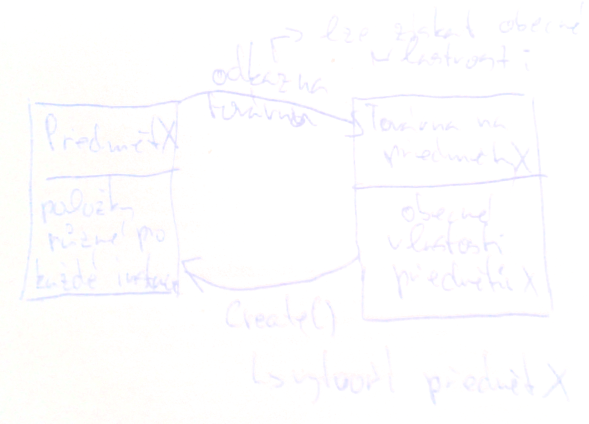
\includegraphics[width=\textwidth]{./img/item-factories.png}
\caption{Ilustrace vztahu objektů a jejich továren.}
\label{item-factories}
\end{figure}

Každá továrna na předměty má také následující atributy:
\begin{itemize}
\item hmotnost, 
\item jméno, 
\item kombo - definuje akce, které lze s předměty provádět,  
\item definice míst v inventáři, kam lze předmět uložit. 
\end{itemize}

\section{Reprezentace komb a akcí}
Každý typy akce definuje svoji továrnu, která je uložena v jádře enginu\vref{engine-core} - jako je tomu v případě předmětů.
Tyto továrny obsahují vlastnosti o dané akci\vref{action-combos}, které také určují požadavky pro provedení dané akce.
Pomocí továrny lze pak vytvořit samotný objekt reprezentující konkrétní akci, kterou lze následně vyvolat určitým 
směrem(sever, východ, jih, západ). Jak podmínky vytvoření akce, tak její provedení je naimplementováno dle dekompilovaných
zdrojových kódů\cite{DMDecompilation} originální hry. Každá továrna na předměty má potom specifikovaný seznam typů akcí,
které lze s předměty provádět.

\section{Reprezentace kouzel}
V jádře enginu jsou uloženy všechny symboly, včetně power symbolů\vref{magic-symbols}.
Tyto symboly mají definovány, kolik je třeba many pro jejich vyvolaní při daném power levelu.
Každé kouzlo potom definuje svoji továrnu, která je rovněž uložena v jádře enginu\vref{engine-core} - stejně jako je tomu v případě předmětů a akcí.
Objekt reprezentující kouzlo lze pak opět vytvořit pomocí jeho továrny. Pro vyvolání kouzla je potom třeba určit směr a entitu,
která kouzlo vyvolává. Vyvolávání a provádění kouzel je opět naimplementováno dle dekompilovaných
zdrojových kódů\cite{DMDecompilation} originální hry. Modifikace vlastnosti entity při vyvolávání symbolů
kouzla pak zajišťuje speciální manager. 

\section{Builder herních úrovní}

Aby bylo možné sestavovat herní úrovně z různých vstupní formátů\aref{aim-builders}, bylo nutné tuto část vyčlenit do samostatného
objektu, který je pak předán jádru enginu\vref{engine-core-section}. Tento objekt budeme dále nazývat builder. Jádro enginu
po builderu vyžaduje vytvoření herních úrovní, přičemž mu předá sadu továren - která je rovněž uložena v jádře. Builder
by se měl také starat o kešování načtených úrovní, jelikož je engine po něm může požadovat několikrát. Objekt builderu
je předán jádru enginu při jeho vytváření, tímto způsobem je možné jádru předat vlastní implementaci builderu.

Tato práce obsahuje pouze jeden builder, který je schopný sestavit herní úrovně z datového objektu popsaném v sekci \ref{level-parsing}.
V sekci \ref{tile-representation} se došlo k závěru, že dlaždice zdí nebudou v tomto enginu existovat. Z toho důvodu jsme se 
v prvních fázích projektu rozhodli při vytváření herní úrovně procházet pouze dlaždice, které jsou od pozice hráče přístupné.
Toho bylo docíleno použitím algoritmu prohledávání do hloubky. Nicméně později se ukázalo, že některé nepřístupné části herní úrovně
jsou používané teleporty nebo přepínači. Z toho důvodu se od tohoto způsobu procházení dat dlaždic upustilo a nyní se procházejí 
postupně všechny dlaždice.

Pro transformování dat na objekty srozumitelné enginu se používají ještě další pomocné subbuildery\cc{sub-builders}. 
Samotné sestavování herní úrovně potom probíhá následovně. V cyklu jsou vytvářeny všechny dlaždice - přitom se za pomocí továren 
z jádra enginu provádí vytváření veškerých objektů, které dlaždice obsahuje.

\begin{figure}[H]\centering
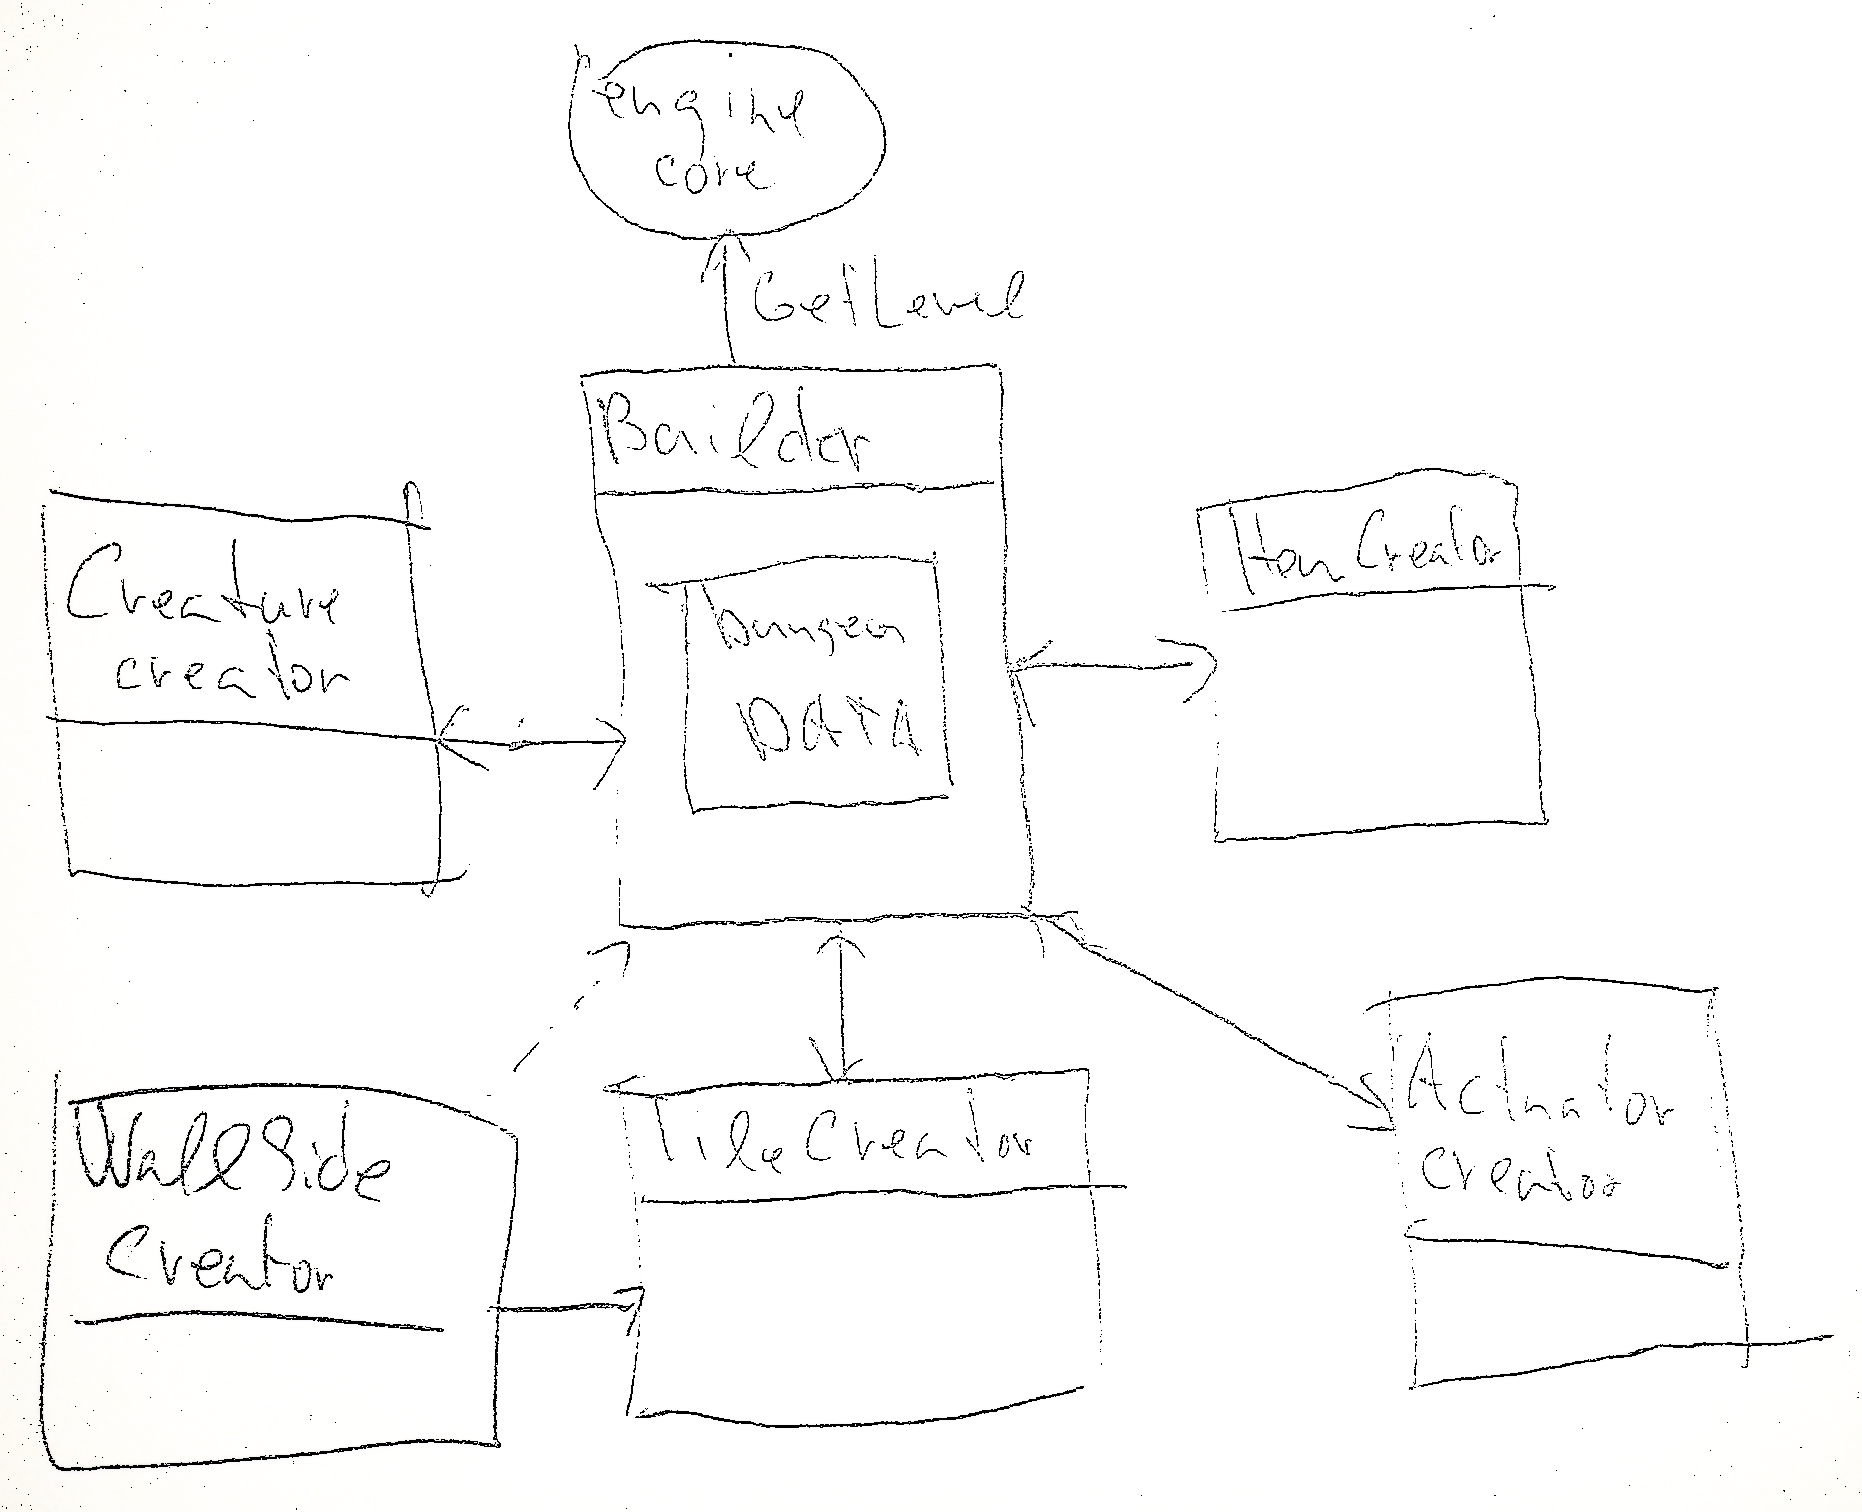
\includegraphics[width=\textwidth]{./img/sub-builders.png}
\caption{Ilustrace struktury builderu.}
\label{sub-builders}
\end{figure}


\section{Inicializace objektů}\label{level-inicialization}

Tento projet si klade za cíl\aref{aim-extensibility} vytvořit co nejlepší objektový návrh. Jedním z faktorů, který by měl takový návrh
zahrnovat je, že veřejné budou jen nezbytně nutné položky tříd. Na to navazuje problém s inicializací takových tříd. 
Například přepínače potřebují referenci na cílovou dlaždici, ale zároveň jsou obsahem dlaždic, je tedy třeba oddělit fázi inicializace 
dlaždic od inicializace přepínačů. Nicméně potom nelze přepínače předat do dlaždic v konstruktoru a tím pádem je pro tuto akci třeba 
vytvořit veřejnou funkci nebo vlastnost, která tak provede. Tato funkce pak narušuje náš cíl, protože tuto funkci může kdokoliv
zvolat později, kdy už to není validní. Z toho důvodu jsme přišli s konceptem tzv. inicializátorů.

Inicializátor je datová třída obsahující vlastnosti, které by běžně byly parametry konstruktoru inicializovaného objektu.
Místo těchto parametrů je do konstruktoru předán inicializátor, který má také události vyvolané
při inicializaci a při dokončení inicializace. Třída beroucí inicializátor jako parametr konstruktoru se zaregistruje na tyto události a
tím pádem není nutná žádná přebytečná položka ve třídě pro inicializátor. Události jsou pak volané skrze metodu v inicializátoru.
Inicializátorem inicializovaná třída si z něj nakopíruje parametry a odhlásí událost. Od té chvíle už není možné třídu modifikovat.
Data inicializátoru se tedy mohou postupně naplňovat a po jejich naplnění se inicializace provede zavoláním metody na inicializátoru.
S využitím asynchronních metod je navíc možné vyvolat inicializaci prvku (např. přepínačů, které potřebují reference na dlaždice) 
již při vytváření dlaždic. Což vede k přehlednějšímu kódu a celkově k inicializaci cyklických struktur bez nutnosti přebytečných 
veřejných položek. 

S využitím dědičnosti inicializátorů je možné nasimulovat volání rutin konstruktorů, tak jak je v C\#  běžné. Na každé úrovní dědičnosti
se využijí některé vlastnosti inicializátoru. Nechť inicializátor B
je potomek inicializátoru A v hiearchii dědičnosti. Nechť C a D jsou třídy, které chceme inicializovat a zároveň D je potomkem C.
Také platí, že konstruktor třídy D vyžaduje inicializátor třídy B a konstruktor třídy C vyžaduje inicializátor A. Potom inicializátor B můžeme
použít pro oba konstruktory tříd C i D. Přičemž na každé úrovni dědičnosti inicializátoru může být zvláštní inicializaci oznamující událost.
Pokud tedy inicializátor volá inicializační události ve správném pořadí, může to nasimulovat pořadí inicializace běžné u konstruktorů.
Při inicializaci dlaždic je právě tento způsob používán. Celou situaci znázorňuje obrázek \ref{initializer-inherence}.

\begin{figure}[H]\centering
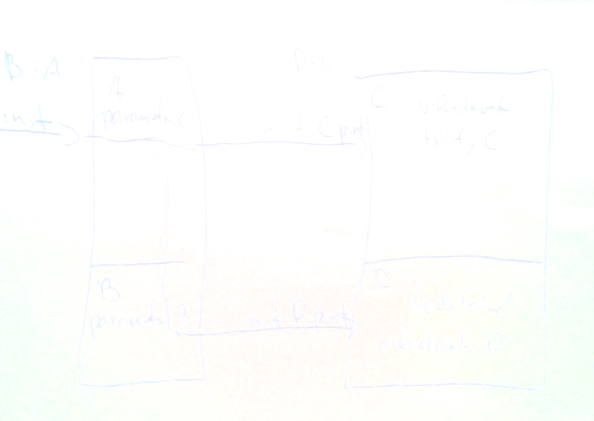
\includegraphics[width=\textwidth]{./img/initializer-inherence.png}
\caption{Ilustrace použití inicializátoru.}
\label{initializer-inherence}
\end{figure}

\section{Renderování a interakce}\label{renderer-interactor}
Dalším cílem\aref{aim-rendering} tohoto projektu je oddělit v enginu zobrazovací vrstvu, tak aby ji bylo možné jednoduše nahradit za jinou.
Se zobrazovací vrstvou nicméně úzce souvisí, jakým způsobem bude prováděna interakce s objekty, proto je v této vrstvě zahrnuta i ona. 
Každý objekt, který to vyžaduje má vytvořený vlastní renderer-interactor na míru. Jak renderer vypadá uvnitř je zpravidla na programátorovi. 
Nicméně obvyklý přístup je takový, že renderer má referenci na konkrétní renderovaný objekt. Podle jeho zpravidla readonly vlastnosti potom určuje
chování vykreslovaní nebo interakce. Pokud se jedná o renderery pro statické objekty(např. dlaždice), tak se zpravidla pozicování určuje relativně
vůči rodiči. Zobrazovací vrstva v tomto enginu nemá stejný grafický výstup jako originální hra, nicméně nic nebrání tomu napsat 
 tuto vrstvu tak, aby jí odpovídala.

\chapter{Vývojová dokumentace}
Následující sekce této kapitoly popisuje třídy reprezentující jednotlivé části enginu a vztahy mezi nimi.

\section{Jádro enginu - \ccc{DungeonBase}}
Jádro enginu reprezentuje třída \ccc{DungeonBase}. Jak již bylo zmíněno v analýze\vref{engine-core-section}, jádro
se skládá ze tří důležitých komponent, které do něj lze předat při jeho vytváření. 
Za těmito komponentami stojí následující rozhraní:

\begin{itemize}
\item \ccc{ILeader} - reprezentuje hráče a jeho skupinu, kterou lze skrze něj ovládat.
\item \ccc{IFactories} - obsahuje továrny pro tvorbu předmětů, nepřátelských entit, kouzel, akcí a definuje úrovně osvětlení.
\item \ccc{IDungeonBuilder} - vytváří pro engine herní úrovně.
\end{itemize}

Pro reimplementaci hry Dungeon Master jsou pak použity následující třídy \ccc{LegacyLeader},
\ccc{LegacyFactories}, \ccc{LegacyMapBuilder}. Konkrétní typy implementací rozhraní
\ccc{ILeader} a \ccc{IDungeonBase} lze předat jádru jako typové parametry.
Případný front end potom může skrze instanci jádra pracovat přímo s konkrétními typy\cc{frontend-core}. Tento projekt
neobsahuje žádné uživatelské rozhraní, namísto něho je pro udávání některých příkazu použita konzole \ccc{GameConsole}.

\begin{figure}[H]\centering
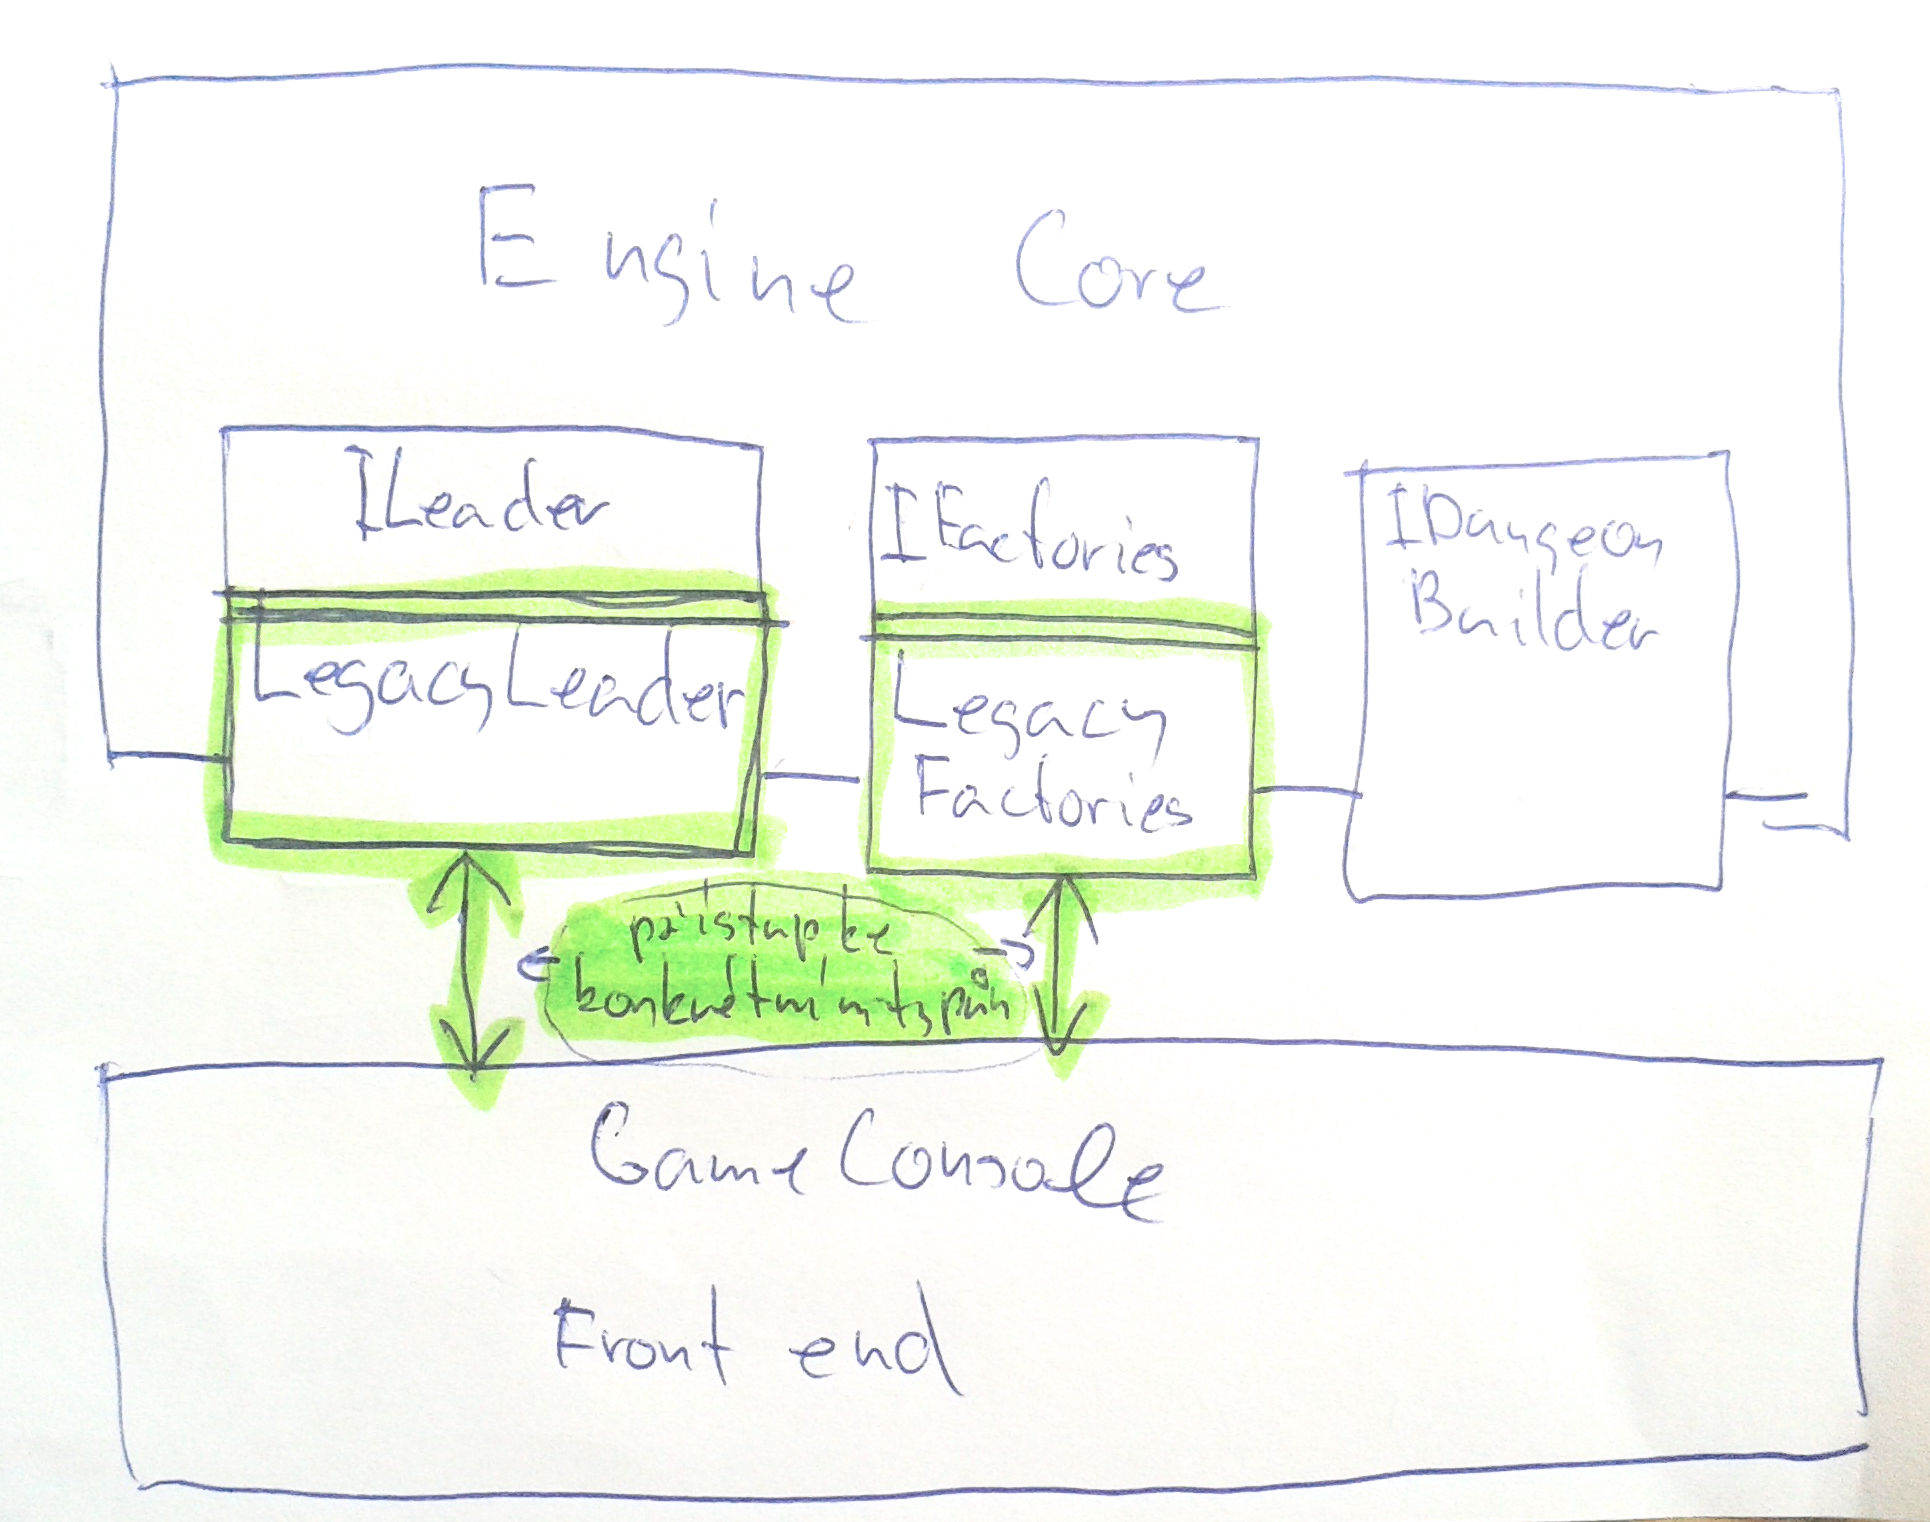
\includegraphics[width=\textwidth]{./img/frontend-core.png}
\caption{Ilustrace komunikace frondendu s jádrem enginu. }
\label{frontend-core}
\end{figure}

\subsection{Správa herních úrovní a dlaždic}\label{engine-level-management}
Při inicializaci jádra je na objektu hráče zaregistrována událost \ccc{ILeader.LocationChanged}, která
je vyvolána po přesunu hráče na novou dlaždici. Zaregistrování resp. odregistrování události se provede po
přiřazení hodnoty do vlastnosti \ccc{Leader}. V obsluze této události se pak provede aktualizace
viditelných dlaždic pomocí funkce \ccc{UpdateVisibleTiles}. K nalezení viditelných dlaždic tato funkce používá
třídu \ccc{RendererSearcher}, která je potomkem třídy \ccc{BreathFirstSearch}. Nalezené dlaždice se
uloží do protected proměnné \ccc{currentVisibleTiles}. V dalším kroku je zavolána funkce 
\ccc{SetupLevelConnectors}, jenž projde všechny viditelné dlaždice vedoucího do jiných úrovní. Pro
každou tuto dlaždici dojde pak voláním funkce \ccc{ConnectLevels} k propojení dané dlaždice s další
úrovní. Poslední akcí je přiřazení úrovně, v které se hráč vyskytuje, do proměnné \ccc{CurrentLevel}.
Popsané akce ilustruje diagram \ref{core-tileUpdate}.

Funkce \ccc{ConnetLevels} načte danou úroveň pomocí funkce \ccc{LoadLevel}, která tak učiní skrze builder.
Načtená úroveň je pak uložena do kolekce \ccc{ActiveLevels}, ve které jsou vždy tři poslední úrovně.
Dlaždice, které propojují herní úrovně, by měli implementovat rozhraní \ccc{ILevelConnector}.
Funkce \ccc{ConnectLevels} pak nastaví cílovou dlaždici do vlastnosti \ccc{ILevelConnector.NextLevelEnter}.
Dlaždice implementující toto rozhraní by měla zajistit její propojení s dlaždicí \ccc{ILevelConnector.NextLevelEnter}.
Všechny funkce zmíněné v této sekci jsou virtuální, a proto je možné jejich chování upravit přetížením.

\begin{figure}[H]\centering
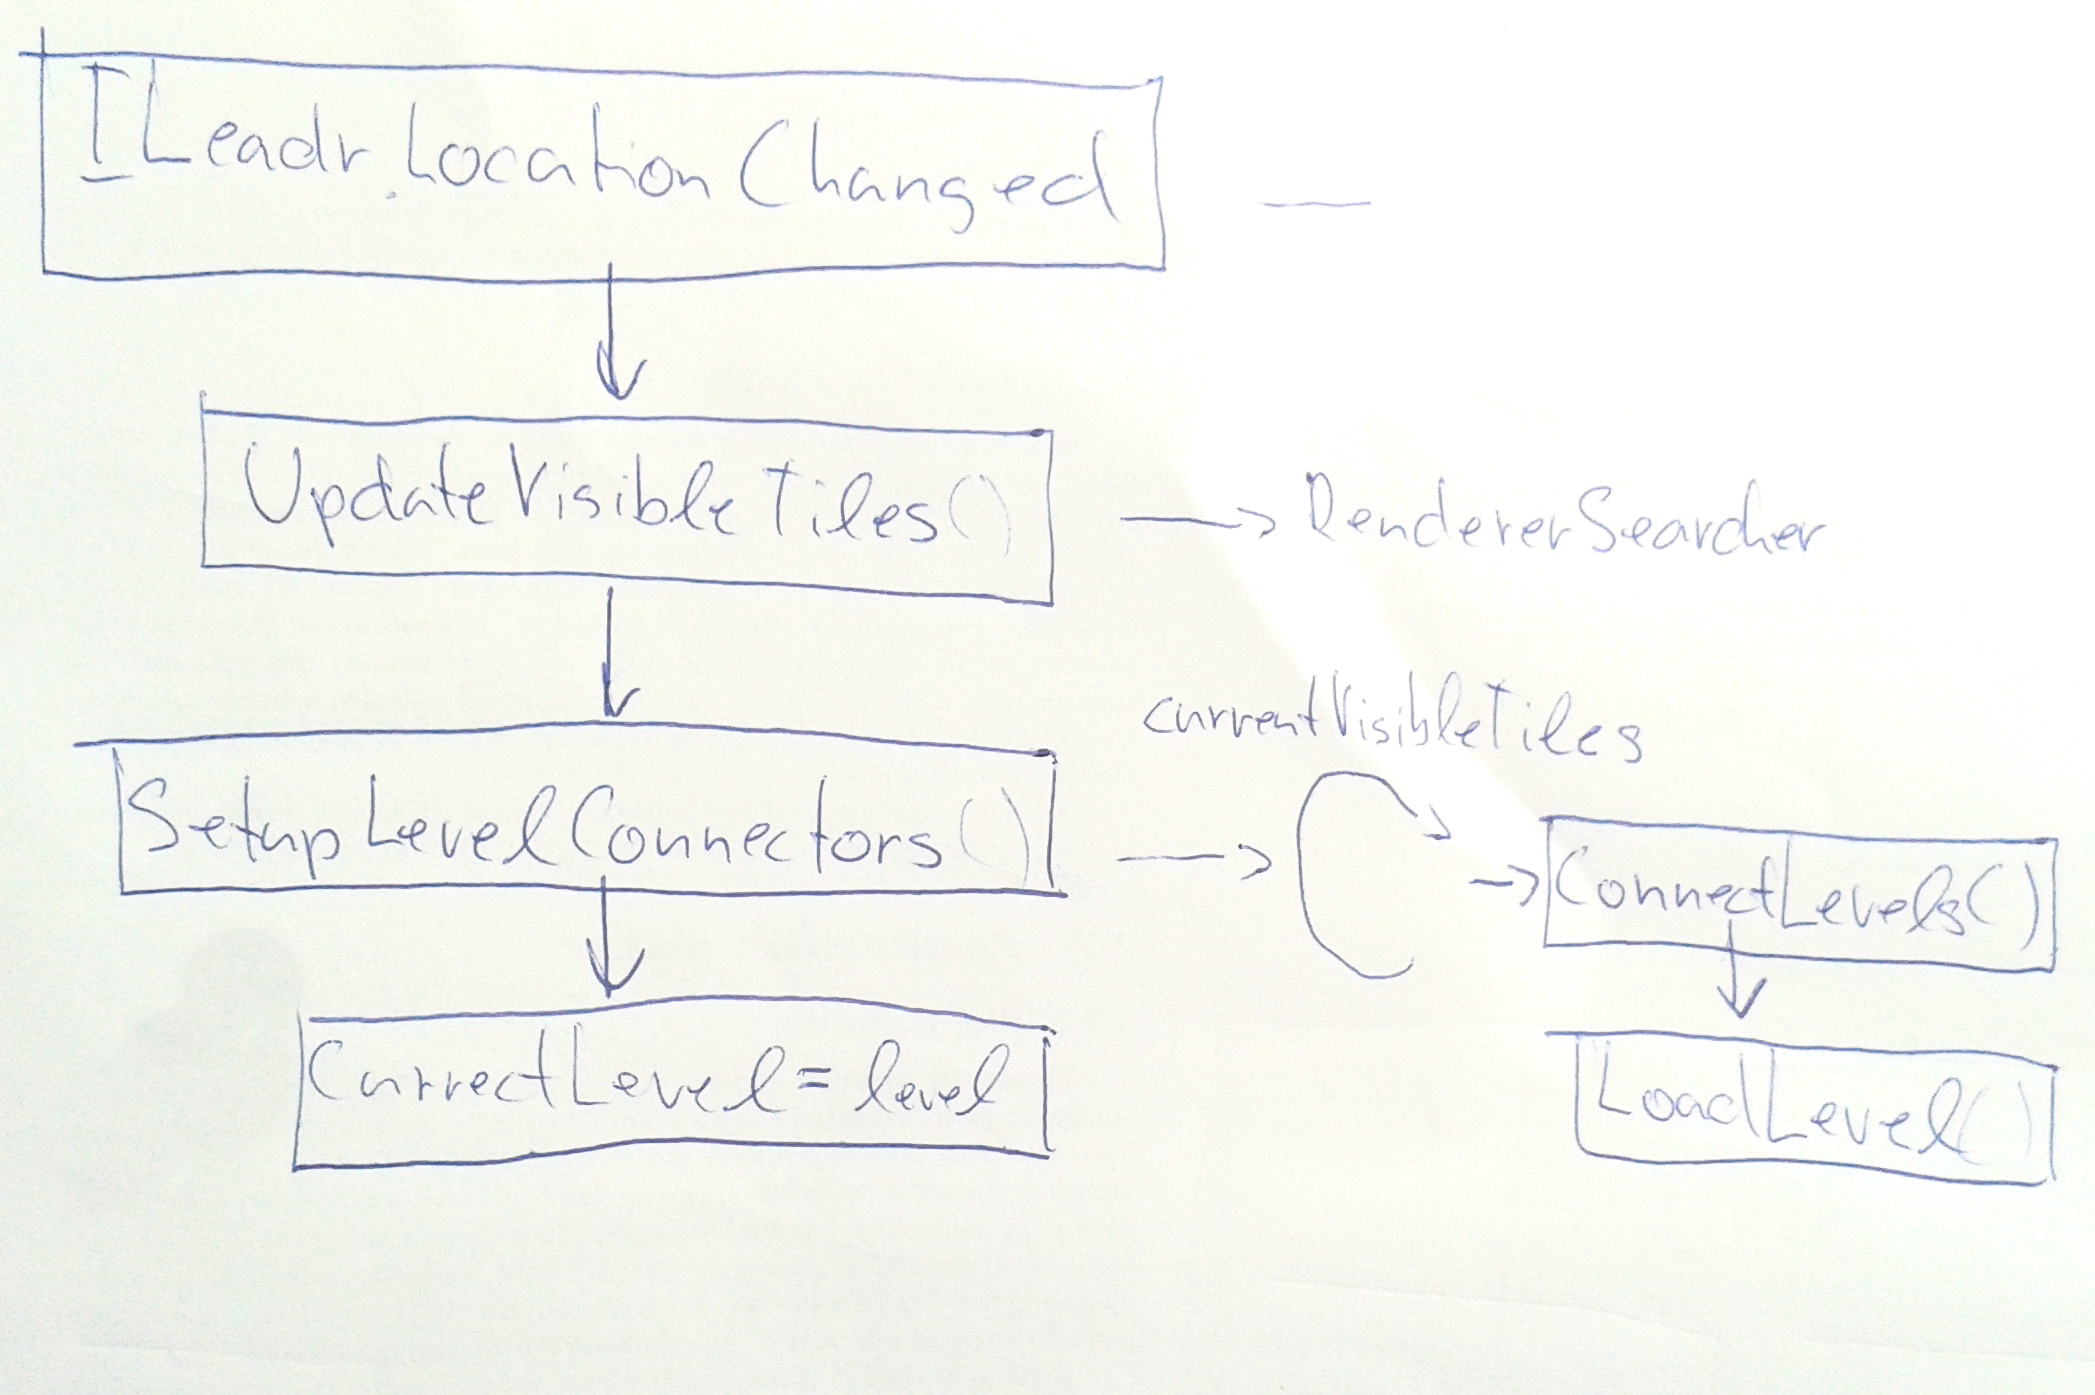
\includegraphics[width=\textwidth]{./img/core-tileUpdate.png}
\caption{Ilustrace funkce jádra. }
\label{core-tileUpdate}
\end{figure}

\subsection{Aktualizace a rendering}
MonoGame zajišťuje herní smyčku, skrze kterou je pak třeba na enginu volat funkce \ccc{Update} a \ccc{Draw}.

V každém zavolání funkce \ccc{Update} se provede aktualizace všech herních úrovní v kolekci \ccc{ActiveLevels}.
Herní úroveň reprezentuje typ \ccc{DungeonLevel}, který má v sobě uložené dlaždice, obtížnost a objekty vyžadující
aktualizaci - které se u něj zaregistrovaly\vref{engine-core-section}. Funkce \ccc{DungeonLevel.Update} pak 
zavolá na všech zaregistrovaných objektech  funkci \ccc{IUpdate.Update}. Všechny tyto objekty musí implementovat
rozhraní \ccc{IUpdate} a musí se sami starat o odregistrování z kolekce, když už aktualizaci nevyžadují. Dále je volána 
funkce \ccc{ILeader.Update} na hráči. Při každém provedení aktualizace se ještě zavolá virtuální funkce 
\ccc{UpdateLight}. Proces reprezentuje obrázek \ref{core-update-draw}.

Funkce \ccc{UpdateLight} přiřadí do proměné \ccc{Light} hodnotu určující úroveň světla, která je v setteru
vlastnosti přepočítána na vzdálenost, po kterou se vykreslují dlaždice. Getter pak vrací již samotnou vzdálenost,
nikoliv hodnotu světla. Hodnota světla je 0 až 5, kde 0 reprezentuje největší osvětlení. Takto je to nastaveno
z důvodu kompatibility se zdrojovými kódy originální hry\cite{DMDecompilation}. 
 Funkce projde všechny šampiony v kolekci \ccc{ILeader.PartyGroup} a nalezne všechny 
objekty implementující rozhraní \ccc{ILightSource}. Na základě hodnot \ccc{ILightSource.LightPower} vypočte 
výslednou hodnotu osvětlení. Tento výpočet lze změnit přetížením funkce. 

V každém zavolání funkce \ccc{Draw} se potom provede vykreslení všech dlaždic v kolekci \ccc{currentVisibleTiles}
skrze jejich renderer\vref{renderer-interactor}. Dále jsou zavolány funkce \ccc{ILeader.Draw} pro vykreslení objektů
ve správě hráče a virtuální funkce \ccc{DrawMiniMap()}, která provede vykreslení minimapy.

\begin{figure}[H]\centering
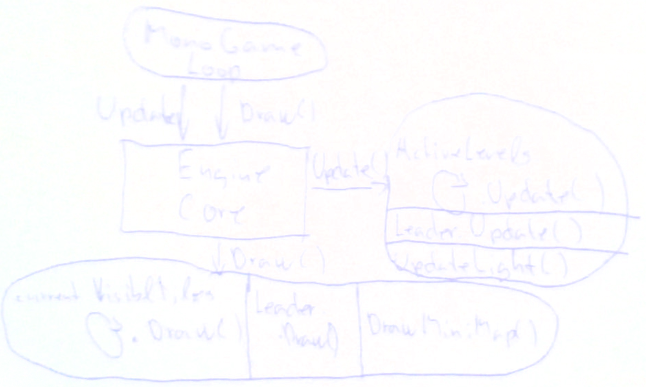
\includegraphics[width=\textwidth]{./img/core-update-draw.png}
\caption{Ilustrace aktualizace a vykreslování z pohledu jádra. }
\label{core-update-draw}
\end{figure}


\section{Dlaždice - \ccc{ITile}}
Nejobecnější strukturu dlaždice definuje rozhraní \ccc{ITile}. Každá dlaždice musí mít definované sousedy,
to zajišťuje položka \ccc{Neighbors} typu \ccc{TileNeighbors}. Tento typ implementuje rozhraní \ccc{INeightbors},
které vyžaduje pouze enumerátor dvojic se směrem a dlaždicí. Směr reprezentuje struktura \ccc{MapDirection}, kde
se jednotlivé směry dají získat skrze její statické členy. Třída \ccc{TileNeighbor} potom implementuje ještě
pomocné funkce a vlastnosti pro jednoduší práci se sousedy. Pomocí této vlastnosti se objekty mohou pohybovat
mezi dlaždicemi. Po vstupu objektu na dlaždici je třeba zavolat na předchozí dlaždici funkci \ccc{OnObjectLeft} a
na nové dlaždici funkci \ccc{OnObjectEntered}. Díky tomu může dlaždice reagovat na vstup resp. odchod objektů -
což je použité například pro přepínače na podlaze. Další vlastností dlaždice je \ccc{LayoutManager}, který 
musí používat entity při pohybu po dlaždicích a mezi nimi. \ccc{LayoutManager} je třída poskytující správu prostoru
na dlaždici, tak aby každý prostor zaujímala pouze jedna entita\vref{layout-manager-section}. Před pohybem entity je
tedy ještě třeba zarezervovat skrze \ccc{LayoutManager} cílový prostor na dlaždici a po dokončení pohybu
je naopak třeba uvolnit prostor předchozí\cc{layout-reserve}. Poslední položkou potřebnou pro pohyb mezi dlaždicemi je vlastnost
\ccc{IsAccessible}, která určuje, zda lze na dlaždici vstoupit.

\begin{figure}[H]\centering
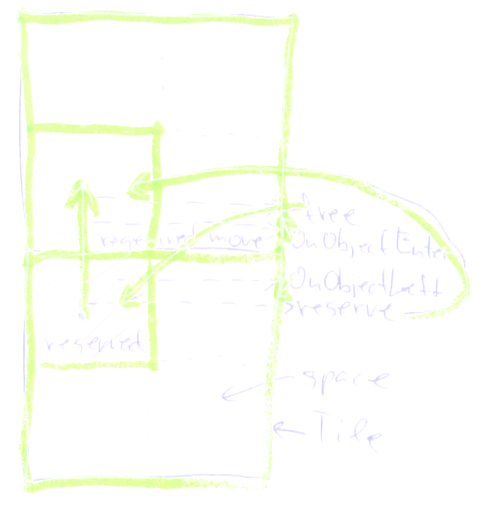
\includegraphics[width=\textwidth]{./img/layout-reserve.png}
\caption{Ilustrace pohybu mezi prostory a dlaždicemi. }
\label{layout-reserve}
\end{figure}

Pro implementaci funkce přepínačů je třeba zajistit komunikaci mezi dlaždicemi\vref{actuator-message-representation}.
Za tímto účelem obsahuje dlaždice vlastnosti pro změnu jejího stavu. Buď lze obsah dlaždice aktivovat přímo
pomocí funkce \ccc{ActivateTileContent} resp. \ccc{DeactivateTileContent} nebo pomocí zaslání zpráv, k jejichž
příjetí slouží funkce \ccc{AcceptMessageBase}. Konkrétní stav je obsahuje pak vlastnost \ccc{ContentActivated}.


V poslední řadě rozhraní reprezentující dlaždice obsahuje prvky: 
\begin{itemize}
\item \ccc{Position} - absolutní pozice od počátku souřadnic,
\item \ccc{GridPosition} - souřadnice dlaždice na mřížce, 
\item \ccc{Drawables} - do této kolekce se mohou zaregistrovat objekty implementující rozhraní \ccc{IRenderable}, 
	které se nechtějí registrovat u dlaždice pomocí funkcí pro vstup a výstup a zároveň se potřebují renderovat, 
\item \ccc{ObjectEntered} resp. \ccc{ObjectLeft} - události vyvolané při vstupu resp. odchodu objektu,
\item \ccc{Level} - reference na level, ve kterém se dlaždice nachází,
\item \ccc{IsInitialized} - určuje, zda je dlaždice plně inicializovaná\vref{level-inicialization},
\item \ccc{Initialized} - tato událost je dlaždicí vyvolána pouze jednou a to v momentě, kdy jsou všechny její části inicializované.
		Tuto událost využívají živé entity k určení doby jejich obživnutí.
\end{itemize}


\subsection{Inicializace dlaždic}
Jak již bylo zmíněno v analýze\vref{level-inicialization}, k inicializaci dlaždic jsou použity tzv. inicializátory. Inicializátor
obsahuje vlastností, které by normálně byly předány jako parametry v konstruktoru. Ovšem v moment předávaní
inicializátoru do konstruktoru, inicializátor ještě nemusí mít naplněné všechny hodnoty. Namísto toho má události \ccc{Initializing}
resp. \ccc{Initialized}, které jsou vyvolány při resp. po inicializaci. Na tuto událost je třeba zaregistrovat
inicializační funkci, která zkopíruje data z inicializátoru do samotného objektu. Pro každou úroveň hierarchie
dědičnosti jsou určeny zvláštní vlastnosti a zvláštní inicializační události. Rodičovské události  inicializátoru jsou vždy
po zdědění rodičovského inicializátoru zakryty novými inicializačními událostmi pro danou úroveň dědičnosti.
Tento způsob je použit pouze pro inicializaci dlaždic. Pro jiné objekty, může inicializátor sloužit pouze jako 
objekt udržující parametry, které jsou hned v konstruktoru inicializované. 

\subsection{Implementace dlaždic}
Částečnou implementaci rozhraní \ccc{ITile} zajišťuje abstraktní třída \ccc{Tile}, která definuje virtuálně \ccc{LayoutManager}.
Dále abstraktně deklaruje kolekci \ccc{SubItems}, která obsahuje všechny objekty na dlaždici. Objekty, které 
implementují rozhraní \ccc{IRenderable}, jsou potom skrze tuto kolekci vykreslovány.
Dlaždice také má tzv. strany, a jsou to buď stěny, strop nebo podlaha\cc{tile-sides}.
Pro tyto strany pak abstraktně deklaruje kolekci \ccc{Sides}, jejímž stěnám pak přeposílá
případné zprávy, které přišly na tuto dlaždici skrze metodu \ccc{AcceptMessageBase}.
Dále implementuje také funkce \ccc{OnObjectEntered} resp. \ccc{OnObjectLeft} tak, že vyvolá jejich odpovídající událost.
Proto je pří případném přetížení těchto funkcí v potomkovi nutné zavolat implementaci rodiče. Všechny
předchozí popsané funkce je možné přetěžovat v potomkovi, a tak přizpůsobit prováděné akce.
V poslední řadě se tento inicializátor stará o inicializaci pozic na mřížce, úrovně a sousedů skrze \ccc{TileInicializator}. 

\begin{figure}[H]\centering
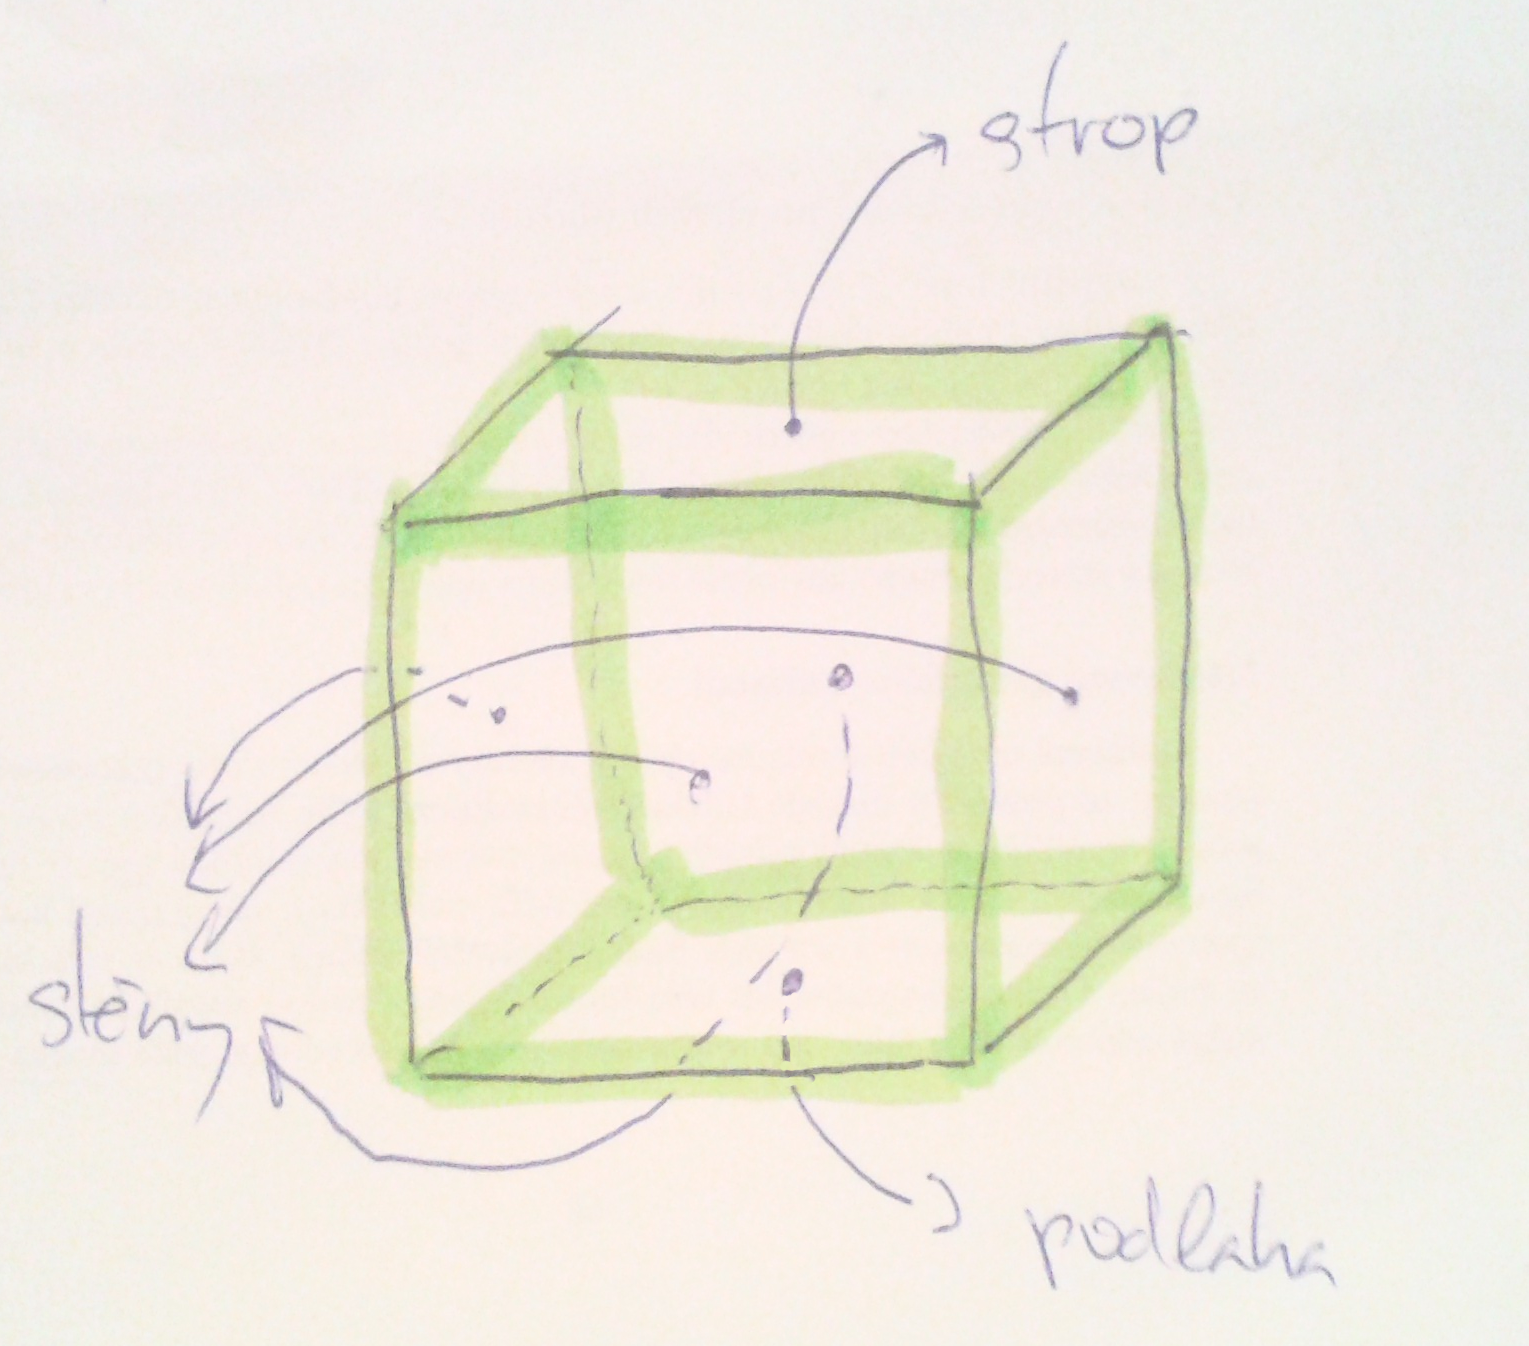
\includegraphics[width=\textwidth]{./img/tile-sides.png}
\caption{3D ilustrace dlaždice a jejích stran. }
\label{tile-sides}
\end{figure}

Přímý generický potomek předchozí třídy \ccc{Tile\textlangle TMessage\textrangle}, kde \ccc{TMessage} je alespoň \ccc{Message},
poskytuje možnost přijímat v potomcích zprávy vlastního typu\vref{actuator-representation}. V případných potomcích teto třídy 
lze naimplementovat funkci \ccc{AcceptMessage}, která přijímá zprávy typu \ccc{TMessage}. Tato třída přetěžuje a zároveň 
uzavírá metodu \ccc{AcceptMessageBase} tak, že deleguje zprávy typu \ccc{TMessage} do metody \ccc{AcceptMessage}. 
Naopak základní implementace metody \ccc{AcceptMessage} je zavolání právě rodičovské implementace \ccc{AcceptMessageBase}. 
Při případném přetěžování této funkce je třeba rozhodnout, zda je nutné volat implementaci rodiče. Všechny dlaždice,
které dědí ze třídy \ccc{Tile\textlangle TMessage\textrangle}, vytváří dva potomky. První z nich je pro případné rozšiřitele,
a proto ponechává typový parametr, druhý pak specifikuje typový parametr na obecný typ \ccc{Message}.

\subsubsection{Dlaždice podlaha - \ccc{FloorTile\textlangle TMessage\textrangle}}
Tato dlaždice implementuje funkci všech jejích stran\cc{tile-sides}. Na stranách, kde
nemá dlaždice sousedy jsou přidány stěny, které mají podporu pro přepínače\vref{dungeon-objects} a dekorace\vref{actuator-analyza}.
Dále je přidána strana na místo stropu a podlahy. Na stranu s podlahou pak může obsahovat přepínač a je na ni možné odkládat
či z ni odebírat předměty. Dlaždice také deleguje veškeré vstupy resp. odchody objektů do samotné strany podlahy
typu \ccc{FloorSide}\vref{tile-sides-section} a to kvůli podpoře odkládání předmětů na zem.

\subsubsection{Další implementace dlaždic}
Další dlaždice převážně využívají dědičností dlaždici podlahy. Výjimkou jsou například schody,
které jsou zároveň příkladem dlaždice implementující rozhraní \ccc{ILevelConnector}. Engine při načtení 
levelu nastaví vlastnost \ccc{ILevelConnector.NextLevelEnter} na odpovídající dlaždici\vref{engine-level-management}.
Při změně předchozí vlastnosti provede dlaždice nastavení sousedů vedoucích do dalšího levelu a používá k tomu vlastní 
implementaci sousedů přetížením vlastnosti \ccc{Neighbors}. Tato možnost je použita ještě u jámy, kvůli propadu do nižšího levelu. 
Rozhraní spojující levely je ještě použito u teleportu, kde při vstupu správného objektu na teleportační dlaždici 
dojde k teleportaci objektu na dlaždici \ccc{ILevelConnector.NextLevelEnter}. Další dlaždicí jsou dveře, které opět 
dědí z podlahy a navíc implementují rozhraní \ccc{IHasEntity}. Toto rozhraní obsahuje vlastnost typu \ccc{Entity},
která reprezentuje neživou entitu na dlaždici. S touto entitou můžou pak pracovat akce, kterými lze dveře rozbít.
Poslední dlaždici reprezentuje třída \ccc{LogicTile}, na kterou nelze vstoupit a slouží pouze jako podpora
pro přepínače\vref{actuators-implementation}.

\subsection{Strany dlaždic - \ccc{ITileSide}}\label{tile-sides-section}
Jak již bylo naznačeno\cc{tile-sides}, dlaždice mohou mít strany, které jsou buď stěny, podlaha nebo strop.
Každou tuto stranu reprezentuje samostatný objekt, který má svůj renderer-interactor\vref{renderer-interactor}. 
Toto rozhraní vyžaduje pouze položku pro renderer a funkci pro přijímání základních zpráv \ccc{Message}. 
Tato funkce je zde z kompatibilních důvodu s originální hrou, kdy texty na zdech mohou být těmito 
zprávami skryty či zobrazeny.

Následuje seznam jednotlivých implementací:
\begin{itemize}

\item \ccc{TileSide} - reprezentuje pouze holou stěnu bez žádných funkcí, která obsahuje
	pouze vlastnost typu \ccc{MapDirection} určující její pozici. 

\item \ccc{ActuatorTileRenderer} - přímý potomkem předchozí strany, který navíc obsahuje přepínač a renderer, 
	jenž se navíc stará o jeho vykreslování a interakci. 

\item \ccc{TextTileSide} - opět přímý potomek první strany, jejíž renderer navíc zobrazuje na zdi text. Viditelnost textu lze změnit zasláním zprávy
	této straně. 

\item \ccc{FloorTileSide} - tato strana obsahuje čtyři úložiště,
na které může hráč pokládat předměty. Je to jedno z míst, kde je potřeba komunikovat s rodičovskou dlaždicí, k tomu
slouží událost \ccc{SubItemsChanged}, která se vyvolá vždy, když byl nějaký předmět odebrán nebo přidán.
Pomocí enumerátoru tohoto objektu je potom možné získat obsažené objekty. Předměty lze pak na podlahu přidávat dvěma 
způsoby, přičemž oba pomocí události informují rodičovskou dlaždici o změně jejího obsahu. První možností je položení 
předmětu přímo z ruky hráče pomocí renderer-interactoru. Druhý způsob je zavolání metody \ccc{OnObjectEntered} resp. \ccc{OnObjectLeft} 
objevující se například při teleportaci nebo hodu předmětu. Celou situaci zobrazuje obrázek \ref{floor-side}.

\item \ccc{ActuatorFloorTileSide} - přímý potomek předchozí strany podlahy, který navíc přidává na podlahu nášlapný přepínač.

\end{itemize}

\begin{figure}[H]\centering
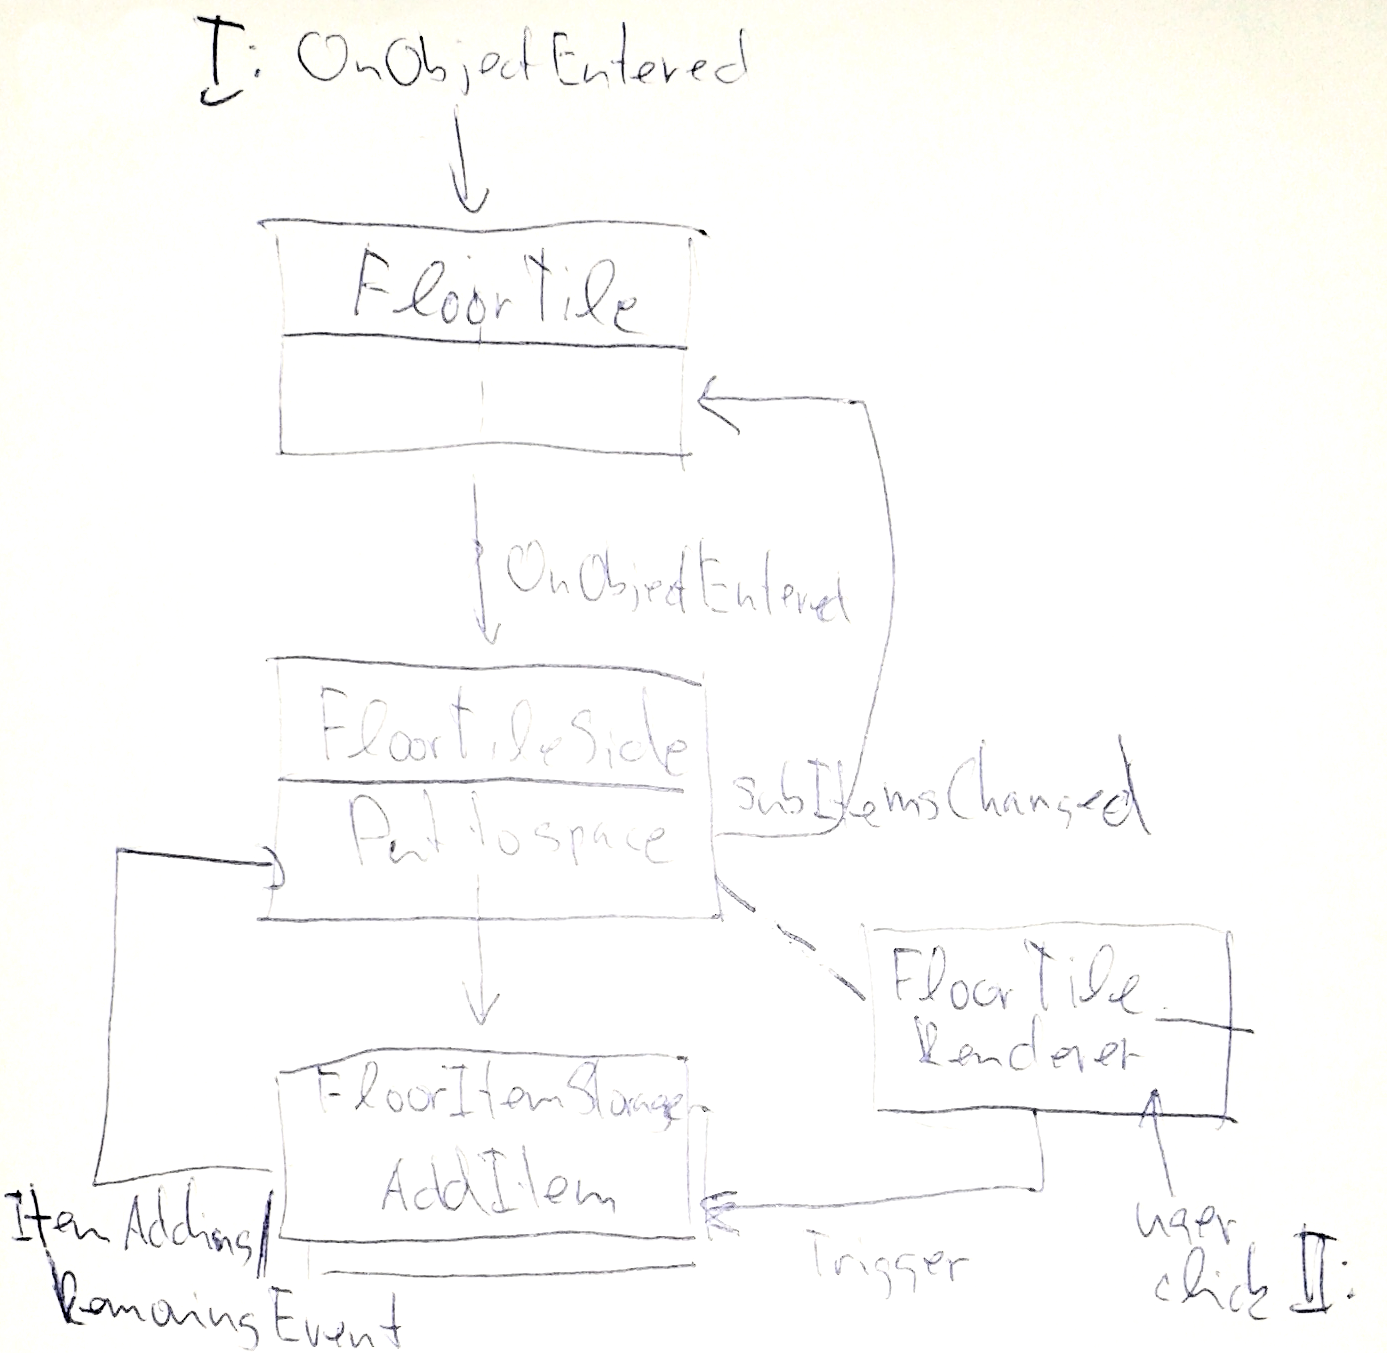
\includegraphics[width=\textwidth]{./img/floor-side.png}
\caption{Ilustrace komunikace podlahy s její dlaždicí při přidávání předmětu. }
\label{floor-side}
\end{figure}


\section{Přepínače - \ccc{IActuatorX}}\label{actuators-implementation}

Za přepínači stojí rozhraní \ccc{IActuatorX}, které vyžaduje pouze API pro příjem zpráv typu \ccc{Message} - pro dodržení
kompatibility s původní hrou. Toto rozhraní pak implementuje třída \ccc{ActuatorX}, která reprezentuje přepínače používající 
pro jejich funkci senzory z originální hry\vref{actuator-analyza}. Kromě toho dále existují implementace přepínačů, které jsou provedeny
jiným způsobem.

\subsection{Implementace obecných přepínačů}
Tato sekce pojednává o přepínačích, které ke své funkci nepoužívají senzory. V tomto enginu jsou použity pro 
dekorace, které provádějí nějakou funkci. K těmto dekoracím v originální hře nenáleží žádné senzory. 
Studií dekompilovaného kódu originální hry\cite{DMDecompilation} se ukázalo, že některé akce jsou fixovány 
na konkrétní typy dekorací. Například pro dekorace s výklenky je naimplementována možnost vkládaní předmětů.
Jelikož tyto dekorace mohou být i součástí senzorů, bylo zapotřebí, aby objekty reprezentující dekorace
implementovali rozhraní \ccc{IActuatorX}, a tak bylo možné naimplementovat funkce pro jejich interakci.

U těchto přepínačů lze zvolit jejich vnitřní formát. Existující implementace jsou:
\begin{itemize}
\item \ccc{DecorationItem} - stará se pouze o rendering dekorace, který zajišťuje třída \ccc{DecorationRenderer}. 
\item \ccc{Alcove} - reprezentuje dekoraci výklenku, o jehož rendering a interakci se stará třída \ccc{AlcoveRenderer}. 
\item \ccc{ViAltairAlcove} - potomek třídy \ccc{Alcove}, který se navíc stará o reinkarnaci šampionů.
\end{itemize}

\subsection{Implementace přepínačů se senzory}
Tyto přepínače se skládají z řady senzorů, které mohou provádět následující akce:

\begin{itemize}
\item změna stavu vzdálené dlaždice,
\item zarotování sekvencí senzorů přepínače\cc{actuator-rotation},
\item přidání zkušeností hráči.
\end{itemize}

Při pokusu o aktivaci přepínače dojde postupně, k aktivaci všech jeho senzorů.
Senzory pak mohou být aktivovány následujícími způsoby:

\begin{itemize}
\item kliknutím myši na dekoraci senzoru, pokud je senzor na zdi, 
\item vstupem resp. odchodem hráčovi skupiny na dlaždici resp. z dlaždice, 
\item zprávou vyslanou jiným senzorem.
\end{itemize}

Více viz sekce \ref{actuator-analyza}.

\subsubsection{Implementace senzorů}

Každý typ senzoru má jinou podmínku aktivace. Senzory se dělí na senzory použité na podlaze, zdi a
na speciální tzv. logické senzory.

Hlavní třídou reprezentující senzor je abstraktní třída \ccc{SensorX}. Tato třída obsahuje společné funkce,
které jsou využívány jejími potomky. Dále také definuje vlastnosti, které lze rozdělit do tří skupin.
Tyto vlastnosti jsou inicializovány inicializátorem\vref{level-inicialization}, který slouží pouze jako datový nosič.
Jde o inicializátor, který reprezentuje třída \ccc{SensorInitializerX}. Pro inicializaci potomků jsou 
používány poděděné implementace tohoto inicializátoru.

Vlastnosti senzorů třídy \ccc{SensorX}:
\begin{itemize}
\item Obecné vlastnosti:
	\begin{enumerate}
	\item \ccc{Delay} - opoždění akce v milisekundách, po kterém se provede akce senzor.
	\item \ccc{LocalEffect} - informace, zda-li je akce určena lokálně pro rodičovskou dlaždici nebo pro vzdálenou.
	\item \ccc{OnceOnly} - informace, zda-li je senzor možné aktivovat pouze jednou.
	\item \ccc{RevertEffect} - u většiny přepínačů obrátí efekt výsledné akce, nicméně přesný význam si stanový vždy konkrétní senzor. 
	\item \ccc{Audiable} - informace určující, zda po aktivaci dojde k přehrání zvuku. (v tomto enginu není použit)
	\item \ccc{GraphicsBase} - reprezentuje dekoraci a zároveň přepínač obecného typu implementující rozhraní \ccc{IActuatorX}.
			Pokus o aktivaci tohoto přepínače se provádí pouze pokud je zobrazena dekorace\cc{decoration-actuator}.
	\end{enumerate}

\item Vlastnosti pro lokální akci:
	\begin{itemize}
	\item \ccc{Rotate} - informace určující, zda-li se má seznam senzorů při aktivaci zarotovat\cc{actuator-rotation}.
	\item \ccc{ExperienceGain} - informace určující, zda-li se mají hráči po aktivaci přidat zkušenosti.
	\end{itemize}

\item Vlastnosti pro vzdálenou akci:
	\begin{itemize}
	\item \ccc{Effect} - určuje jaká zpráva je odeslaná na cílovou dlaždici. (Akce zprávy může být obrácená pokud je nastavena vlastnost \ccc{RevertEffect}).
	Hodnoty efektu jsou následující:
		\begin{itemize}
		\item Aktivace 
		\item Deaktivace
		\item Přepnutí stavu
		\item Drž - tento stav nelze odeslat ve zprávě a je na senzoru, aby ho interpretoval pomocí aktivace či deaktivace.
		\end{itemize}
	\item \ccc{Specifier} - směr použitý v odeslané zprávě, který může být interpretován jako číslo(lze získat pomocí \ccc{MapDirection.Index}).
	\item \ccc{TargetTile} - reference na cílovou dlaždici.
	\end{itemize}
\end{itemize}

Kromě předchozích vlastností obsahuje tato třída funkce pro vykonání akcí senzorů. Pokud je efekt senzoru vzdálený, funkce  \ccc{TriggerEffect} odešle zprávu 
na danou cílovou dlaždici. Jinak provede akci pro lokální efekt, který lze 
také vykonat přímo zavoláním funkce \ccc{TriggerLocalEffect}. Tyto funkce lze použít pouze v potomcích.

Následující třídy jsou přímými potomky třídy \ccc{SensorX}:

\begin{enumerate}
\item\label{floor-tile-sensor} \ccc{FloorSensor} - tyto senzory lze vložit pouze do přepínačů, které mohou být na podlaze.
\item\label{wall-tile-sensor} \ccc{WallSensor} - tyto senzory lze vložit pouze do přepínačů, které mohou být na stěně.
\item \ccc{LogicGateSensor} resp. \ccc{CounterSensor} - pro tyto senzory existuje speciální dlaždice \ccc{LogicGateTile}
\end{enumerate}

Senzory z bodu \ref{floor-tile-sensor} a \ref{wall-tile-sensor} mají funkci \ccc{TryTrigger}, která se pokusí senzor 
aktivovat a pokud uspěje, stará se o provedení efektu. Zda-li se senzor aktivuje stanoví abstraktní funkce \ccc{TryInteract},
kterou implementují potomci. Pro každou variantu senzoru mají funkce odlišné parametry. Pokud je třeba modifikovat způsob 
provedení výsledného efektu, je možné funkce \ccc{TryTrigger} přetížit.

\begin{figure}[H]\centering
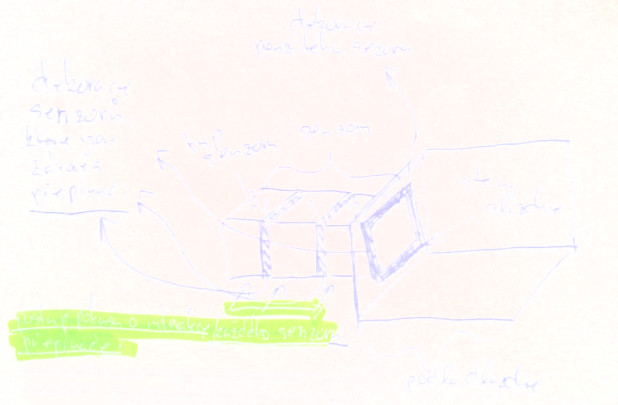
\includegraphics[width=\textwidth]{./img/decoration-actuator.png}
\caption{Ilustrace struktury přepínače se senzory.}
\label{decoration-actuator}
\end{figure}


Kromě předchozích senzorů ještě existují tzv. logické senzory(viz \ref{floor-tile-sensor}). První z nich \ccc{LogicGateSensor} funguje 
jako logické hradlo, které má k dispozici osm bitů. Čtyři z nich jsou nastaveny při designu na hodnoty a ostatní na nuly. 
S druhou čtveřicí lze pak manipulovat pomocí zpráv. Index směru zprávy určuje kolikátý bit se má ovlivnit. A tento bit
je pak ovlivněn akcí zprávy. Pokud jsou obě čtveřice stejné, je vyvolán efekt senzoru. Dalším
senzorem je \ccc{CounterSensor}, který má dané číslo. Aktivační zprávy toto číslo poté navyšují a deaktivační zprávy
ho snižují. Pokud je číslo  nula, je vyvolán efekt.
 
\subsubsection{Implementace přepínačů používající senzory}

Rodiči těchto přepínačů je třída \ccc{Actuator}. Tato třída poskytuje funkci pro zarotování senzory přepínače, která
lze vyvolat pouze z potomků. Zda-li se mají senzory zarotovat se určuje nastavením vlastnosti \ccc{Rotate}, která se po jeho 
provedení nastaví zpět na false. Samotné zarotování se pak provede zavoláním funkce \ccc{ProcessRotationEffect}.

Prvním potomkem předchozí třídy je třída \ccc{FloorActuator}, která může obsahovat pouze senzory určené
na podlahu tj. \ccc{FloorSensor}. Pokus o její aktivaci se provádí funkcí \ccc{Trigger}. Jako první parametr se jí předává objekt,
který vstupuje resp. odchází z dlaždice, dále seznam všech objektů na dlaždici a naposled informace, zda objekt
vstupuje či odchází. Pro přepínač je vytvořena speciální podlaha \ccc{ActuatorFloorSide}, která se stará 
o volání funkce \ccc{Trigger}.

Dalším potomkem je třída \ccc{WallActuator}, která může obdobně obsahovat pouze senzory určené na zeď tj. \ccc{WallSensor}.
Pokus o její aktivaci se provádí opět funkcí \ccc{Trigger}, která má jediný parametr typu \ccc{ILeader}. Pro přepínač
je určena strana \ccc{ActuatorWallTileSide}. Funkce \ccc{Trigger} je pak volána skrze renderer dané strany. 

Předchozí dva přepínače se také starají o interakci s přepínačem dekorace posledního senzoru\cc{decoration-actuator}

Poslední speciální implementací je třída \ccc{LogicActuator}, která může obsahovat logické senzory.
Komunikace se senzory probíhá pomocí zasílání zpráv. Pro tento přepínač je vytvořena speciální dlaždice,
na kterou nelze hráčem vstoupit. Tato dlaždice je reprezentována třídou \ccc{LogicTile}. 

\begin{figure}[H]\centering
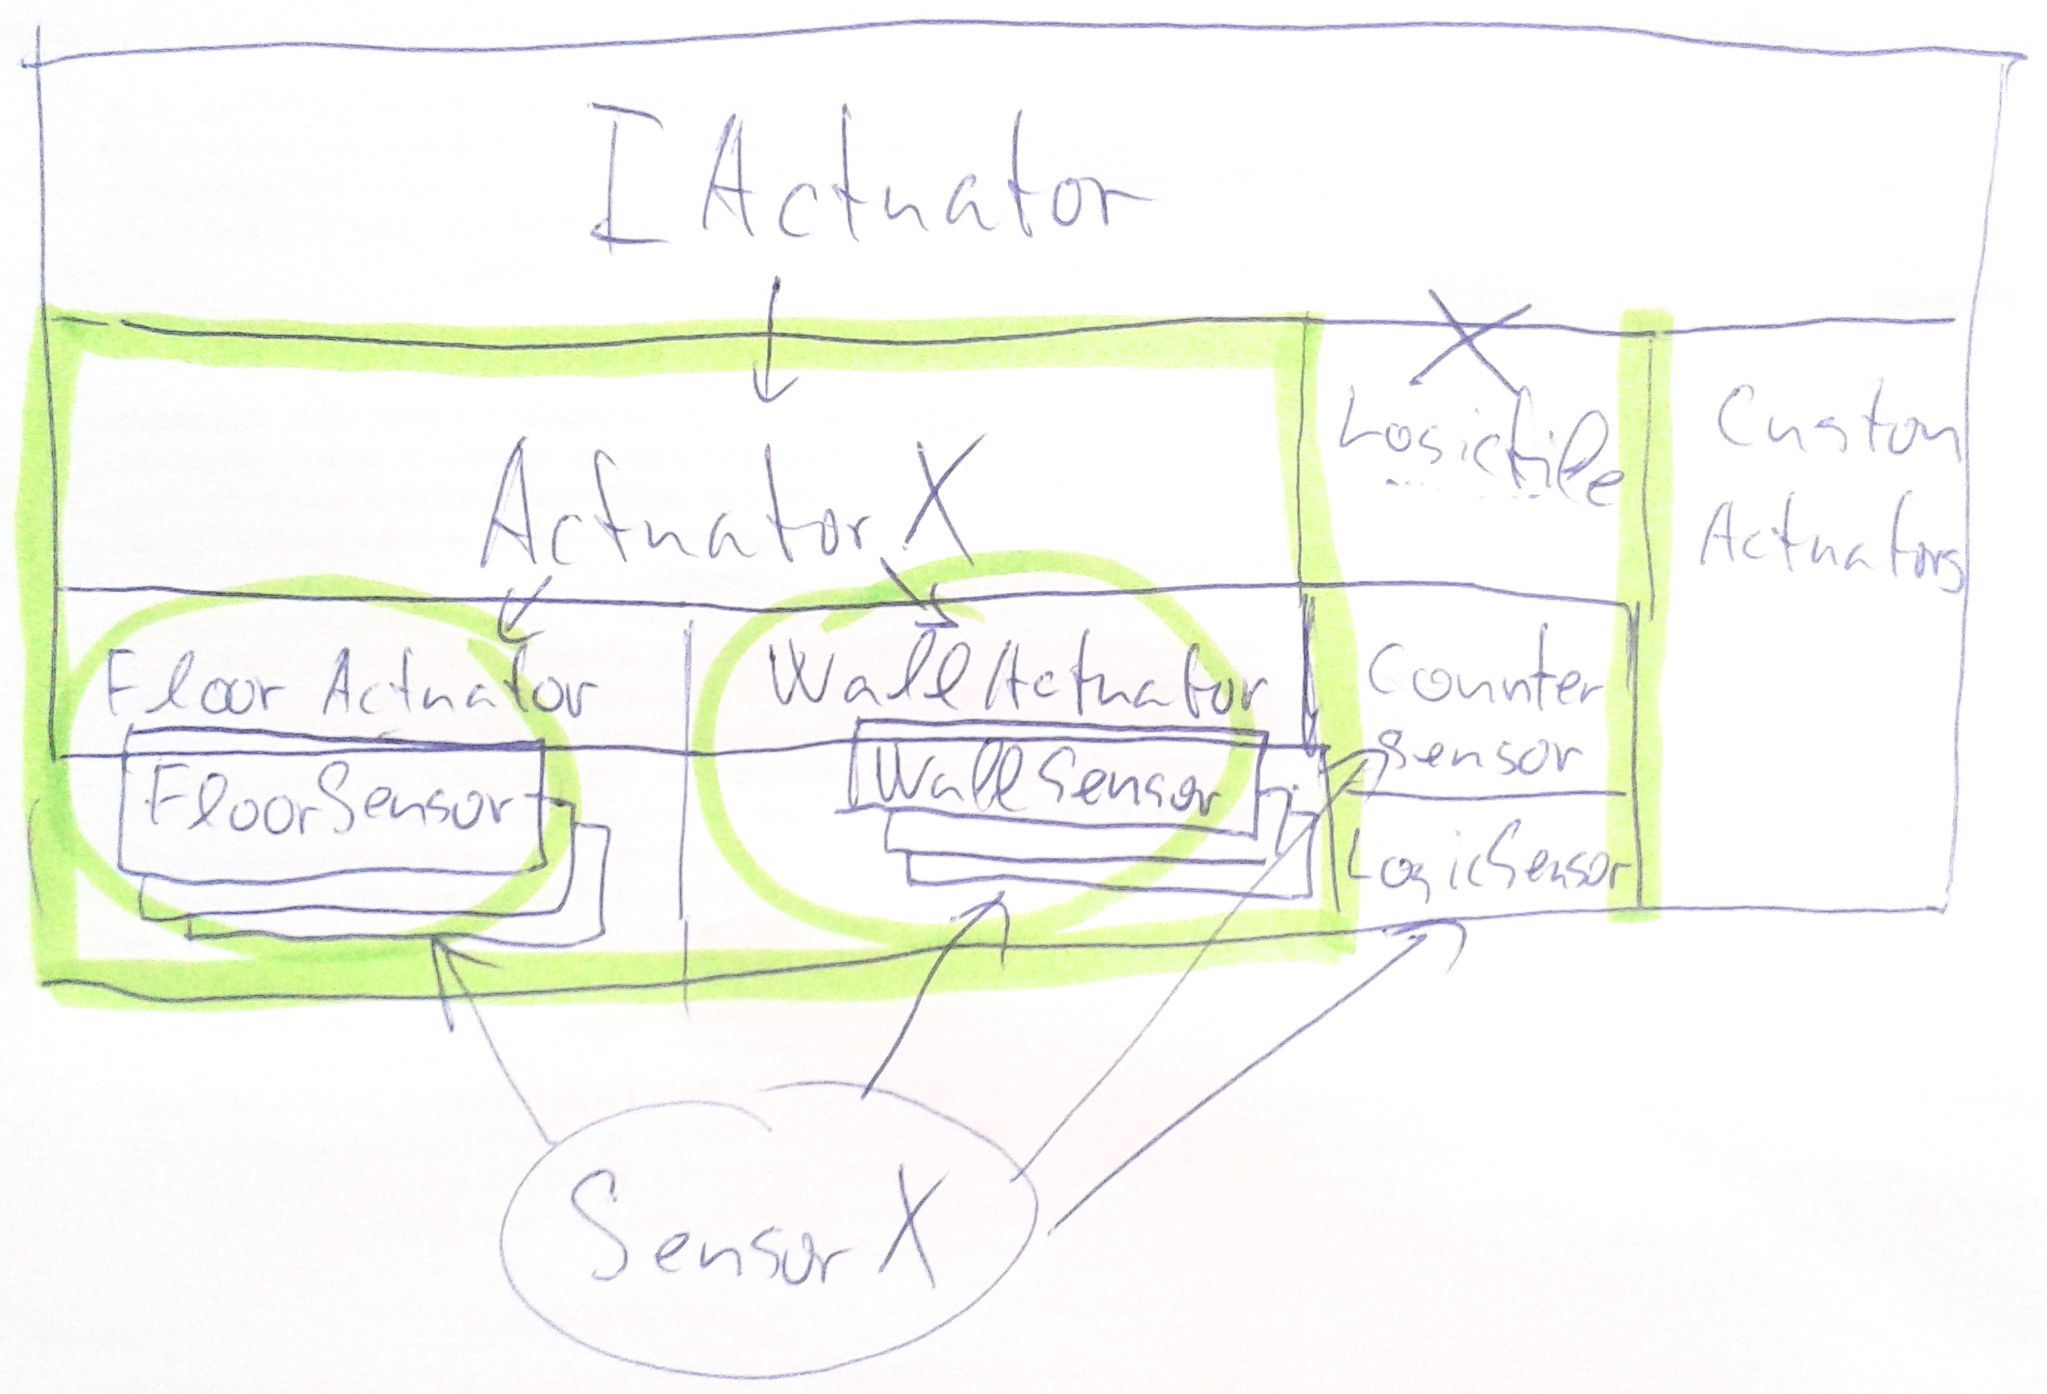
\includegraphics[width=\textwidth]{./img/actuator-sensor-hierarchii.png}
\caption{Ilustrace hierarchie přepínačů a senzorů.}
\label{actuator-sensor-hierarchii}
\end{figure}

\section{Herní entity}

Za deklarací neživých entit stojí rozhraní \ccc{IEntity}, které definuje funkci \ccc{GetProperty} pro získání vlastnosti dané entity.
Za živými entitami stojí naopak rozhraní \ccc{ILiveEntity}, která navíc disponuje funkcí \ccc{GetSkill} pro získání schopností. Dále
také deklaruje:

\begin{itemize}
\item tělo entity
\item způsob rozmístění entity na dlaždici
\item relace s dalšími entitami
\end{itemize}

\subsection{Implementace vlastností entit}

Vlastnost deklaruje rozhraní \ccc{IProperty}. Nejprve obsahuje vlastnost \ccc{Value}, která stanovuje aktuální hodnotu
dané vlastnosti. V jejím getteru a setteru se typicky provádějí kontroly okrajových hodnot a případné reakce na ně. 
Další vlastností je \ccc{BaseValue}, což je aktuální hodnota, které může vlastnost nabýt, pokud není nějak modifikovaná.
Maximální hodnotu včetně modifikací určuje vlastnost \ccc{MaxValue}. Další vlastností je \ccc{AdditionalValues}, která shromažďuje
modifikace dané vlastnosti. Je to sekvence typu \ccc{IEntityPropertyEffect}, která definuje hodnotu a typ dovednosti. Posledním
prvkem rozhraní je typ vlastnosti, který reprezentuje instance implementující rozhraní \ccc{IPropertyFactory}.
Entita na základě tohoto typu potom vrací příslušné vlastnosti. 
Pro usnadnění tvorby unikátních typů existuje generická třída \ccc{PropertyFactory}, která má jako typový parametr typ alespoň \ccc{IProperty}.
Tato třída se řídí vzorem singleton, jejíž jediná instance lze získat přes statickou položkou \ccc{Instance}. Takto lze pak 
generovat typy pomocí třídy reprezentující vlastnost.

Pro usnadnění práce je existuje implementace rozhraní \ccc{IProperty} a to třída \ccc{Property}. Tato třída definuje 
maximální hodnotu jako součet základních hodnoty a sumu modifikujících hodnot. Dále Při nastavení konkrétní hodnoty ořezává
hodnotu do povoleného intervalu, který je mezi nulou a maximální hodnotou. Také definuje událost vyvolanou při změně hodnoty.
Všechny vlastnosti jsou deklarovány abstraktně nebo virtuálně. 

 Některé vlastnosti mohou požadovat přístup k jiným vlastnostem či přístup k rodičovské entitě. V takovém
 případě je na programátorovi, jak takového cíle dosáhne. Typicky se v takovém případě předá v konstruktoru
 potřebná vlastnost nebo se vytvoří událost, která danou závislost deleguje vně. 

 Seznam předdefinovaných vlastností je možné najít ve jemném prostoru \ccc{DungeonMasterEngine.DungeonContent.Entity.Properties}.
 Jak již bylo zmíněno\vref{entity-properties}, může nastat, že daná entita vlastností nedisponuje. V takovém případě 
 je vrácena instance třídy \ccc{EmptyProperty}. 

\subsection{Implementace schopností entit}

Schopnosti deklaruje rozhraní \ccc{ISkill}. První vlastností tohoto rozhraní je \ccc{SkillLevel}, která udává úroveň,
na které je daná schopnost. Do této hodnoty jsou započítány i úrovně získané například kouzelnými předměty. Hodnotu
bez těchto extra úrovní určuje vlastnost \ccc{BaseSkillLevel}. Dále obsahuje vlastnosti \ccc{Experience} a \ccc{TemporaryExperience}
určující dosavadní hodnotu zkušeností. Dále obsahuje vlastnost \ccc{BaseSkill}, což je reference na základní(viz. analýza) schopnost. Pokud
je daná schopnost již základní, je hodnota \ccc{null}. Přidat schopnosti zkušenosti je možné zavoláním funkce \ccc{AddExperience}.
Konkrétní algoritmus přepočítávání zkušeností na levely záleží vždy  na konkrétní implementaci. Stejně jako u vlastností 
i zde existuje vlastnost \ccc{Type}, tentokrát ale typu \ccc{ISkillFactory}. Stejně jako u vlastností, je možné tyto reprezentanty
vytvářet pomocí generické třídy \ccc{SkillFactory}. 

Třída \ccc{SkillBase} implementuje získávání zkušeností schopností jako v originální hře. Všechny schopnosti 
využívající tuto třídu jsou ve jemném prostoru \ccc{DungeonMasterEngine.DungeonContent.Entity.Skill}. Stejně jako
u vlastností i zde entita nemusí mít dotazovanou schopnost. V takovém případě vrací instanci třídy \ccc{EmptySkill}.

\subsection{Tělo - \ccc{IBody}}

Následující API umožňuje pro entity vytvořit různé druhy těl.
Tělo se skládá z částí, které mohou sloužit jako úložiště. Dále pak existují externí
úložiště. API je navržené tak, aby dovolovalo definovat různé druhy úložišť a těl. 
Engine obsahuje pouze implementaci pro lidské tělo tj. třída \ccc{HumanBody}.
Tělo entity je definováno rozhraním \ccc{IBody} a obsahuje následující atributy:

\begin{itemize}
\item \ccc{BodyParts} - obsahuje seznam částí těla,
\item \ccc{Storages} - obsahuje seznam všech úložišť včetně částí těla,
\item \ccc{GetStorage} - funkce pro vyhledání úložiště včetně částí těla,
\item \ccc{GetBodyPart} - funkce  pro vyhledání části těla. 
\end{itemize}

\subsubsection{Inventář - \ccc{IInventory}}
Každý inventář má definovanou vlastnost \ccc{Type}, což je typ úložiště, který reprezentuje instance třídy 
implementující rozhraní \ccc{IStorageType}. Dále pak definuje readonly kolekci \ccc{Storage} pro ukládání předmětů.
A v poslední řadě obsahuje funkce pro přidávaní a odebírání předmětů z úložného prostoru tj. \ccc{TakeItemFrom}, \ccc{AddItemTo}, \ccc{AddItem},
\ccc{AddRange}. Třída \ccc{Inventory} implementuje všechny funkce inventáře a je jí tedy možno přímo použít nebo rozšířit.

\subsubsection{Část těla - \ccc{IBodyPart}}
Část těla je definovaná rozhraním \ccc{IBodyPart}, které je potomkem rozhraní \ccc{IInventory}. Toto rozhraní navíc definuje 
následující vlastnosti: 
\begin{itemize}
\item \ccc{IsWound} - definuje, zda je část těla zraněna,
\item \ccc{InjuryMultipler} - definuje pravděpodobnost zranění části těla.
\end{itemize}

Obecnou implementací rozhraní je třída \ccc{BodyPart}. 

\subsection{Rozmístění entity na dlaždici}\label{layout-manager-section}

Rozhraní \ccc{IGroupLayout} definuje obecně možné rozmístění na dlaždici. Jeho vlastnost \ccc{AllSpaces} obsahuje všechny možné prostory, které daná entita může využít.
Toto prostory rozdělují prostor dlaždice na mřížku\cc{space-grid}, která nemusí být rovnoměrná.
Jednotlivě prostory jsou reprezentovány rozhraním \ccc{ISpace}. Dale API vyžaduje funkci \ccc{GetToNeighbour}, která nalezne cestu skrze prostory
na cílovou sousední dlaždici\cc{space-route}. Funkce \ccc{GetToSide} vrací cestu k libovolné ze stran dlaždice. Jednotlivé články cesty jsou 
reprezentovány rozhraním \ccc{ISpaceRouteElement}. Poslední funkce musí umět vytvořit z prostoru a dlaždice článek cesty,
tedy \ccc{ISpaceRouteElement}.  

\begin{figure}[H]\centering
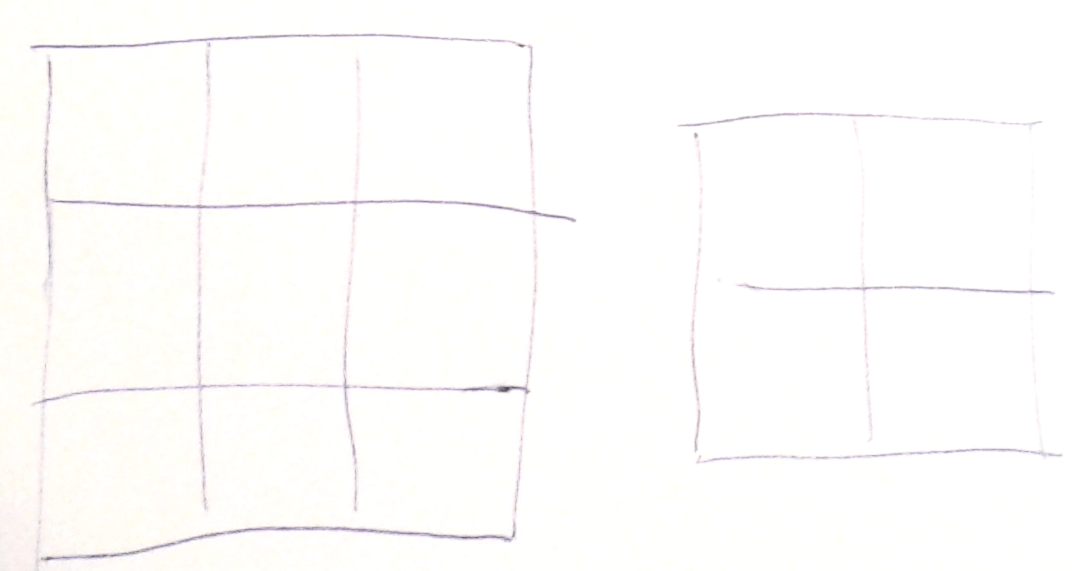
\includegraphics[width=\textwidth]{./img/space-grid.png}
\caption{Ilustrace rozdělení dlaždice na prostory. }
\label{space-grid}
\end{figure}

Rozhraní \ccc{ISpace} musí definovat, jakým stranám dlaždice je prostor přilehlý. Dále musí pomocí obdelníku definovat prostor, který na dlaždici využívá.
Celý prostor dlaždice je pak definovaný na pole o velikosti 1000x1000. Přičemž souřadnice rostou
shora dolů a zleva doprava. Nahoře je pak sever, vpravo východ, dole jih a vlevo západ. Kromě toho také musí definovat sousední
prostory, k čemuž využívá generické rozhraní \ccc{INeighborable}. Ilustrace viz obrázek \cc{tile-spaces}

\begin{figure}[H]\centering
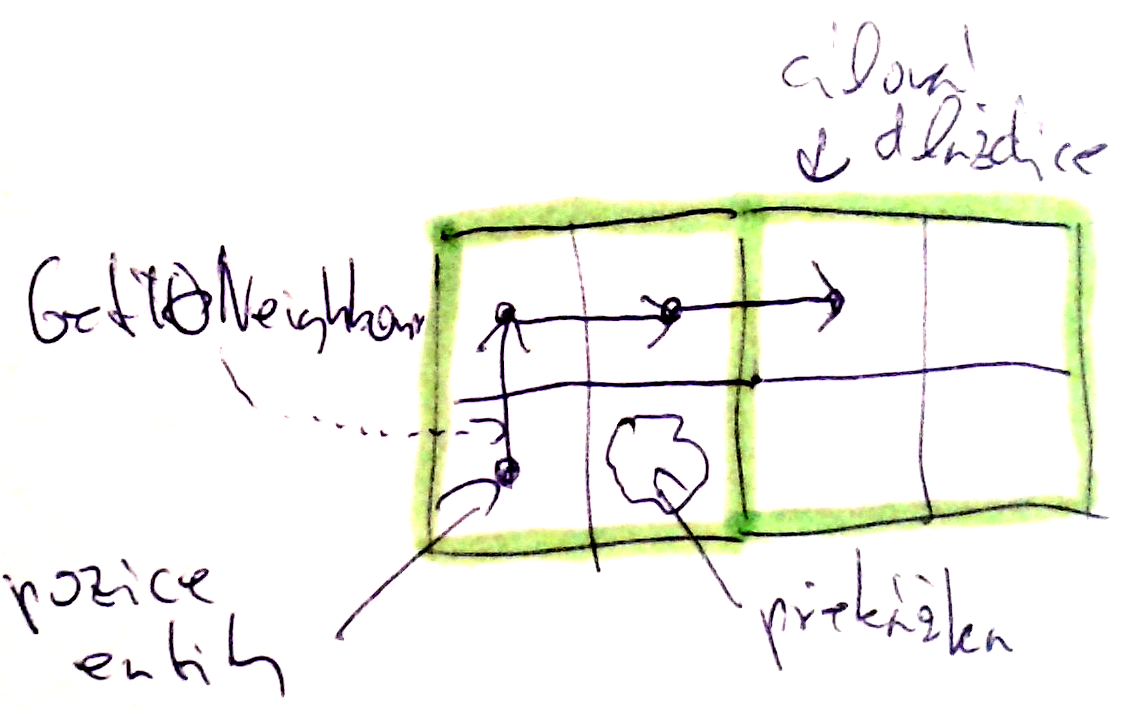
\includegraphics[width=\textwidth]{./img/space-route.png}
\caption{Ilustrace nalezení cesty na sousední dlaždici. }
\label{space-route}
\end{figure}

\begin{figure}[H]\centering
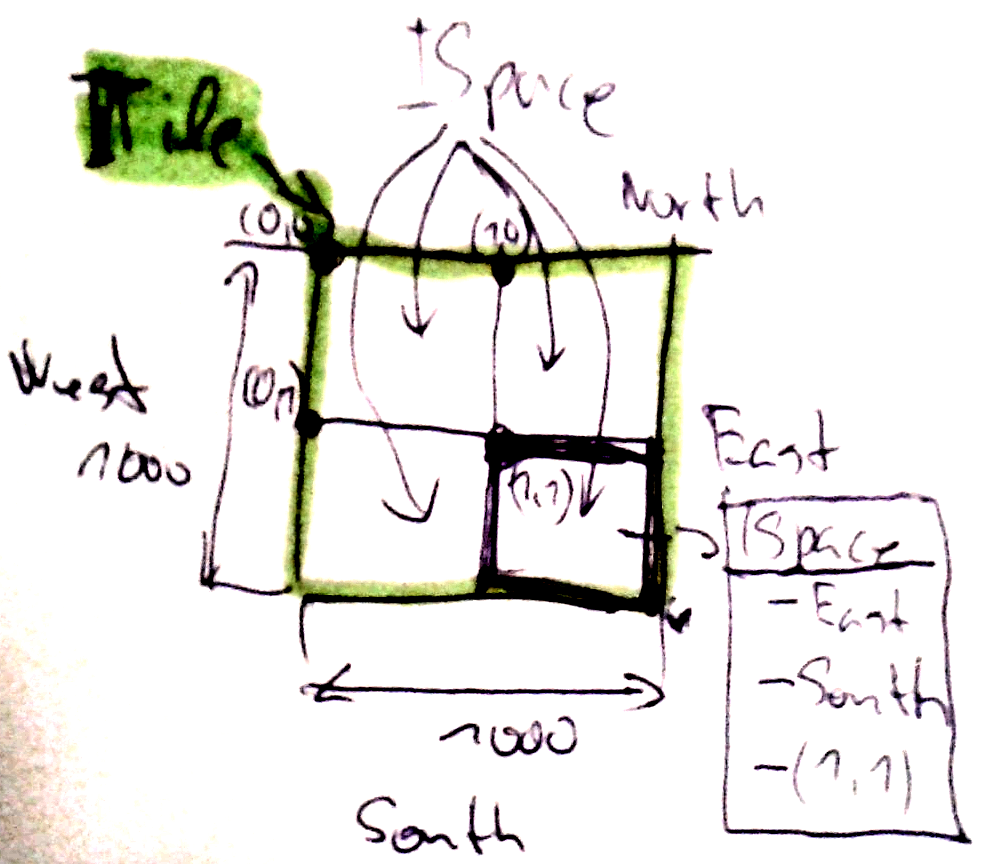
\includegraphics[width=\textwidth]{./img/tile-spaces.png}
\caption{Ilustrace vlastností prostorů. }
\label{floor-side}
\end{figure}

Rozhraní \ccc{ISpaceRouteElement} se potom skládá pouze z prostoru, dlaždice a absolutně pozice, na které má stát daná entita.
Pro výpočet této pozice se může použít pozice dlaždice a prostor. Při při implementaci tohoto rozhraní je možné využít 
předem připravený hledač nejkratších cest pro prostory \ccc{GroupLayoutSearcher}. Pro reprezentaci sousedů prostorů mřížky je tu 
zase tříd \ccc{FourthSpaceNeighbors}.

Celé toto rozhraní je immutable objekt, který pouze definuje prostory na dlaždici a způsob pohybu mezi nimi. Z toho důvodu
instance tříd implementující toto rozhraní mohou být singeltony. Engine definuje layout pro prostor reprezentující celou dlaždici
a pro prostory jako čtvrtiny dlaždice.

\subsubsection{Řízení obsazeného prostoru na dlaždici}

K předchozímu mechanismu je ještě třeba další část, která bude zaznamenávat samotné využité pozice na dlaždici. K tomuto 
účelu existuje třída \ccc{LayoutManager}.  Lze pomocí ní získat seznam entity na dlaždici a seznamy využitých prostorů dlaždic.
Dále poskytuje API pro přidání entity na daný prostor na dlaždici, odebrání prostoru a získání entit, které využívají 
alespoň část nějakého prostoru. Entity s různými rozmístěními mohou být na stejné dlaždici, pokud
je na ní dostatek prostoru pro oba\cc{layout-manager}.

\begin{figure}[H]\centering
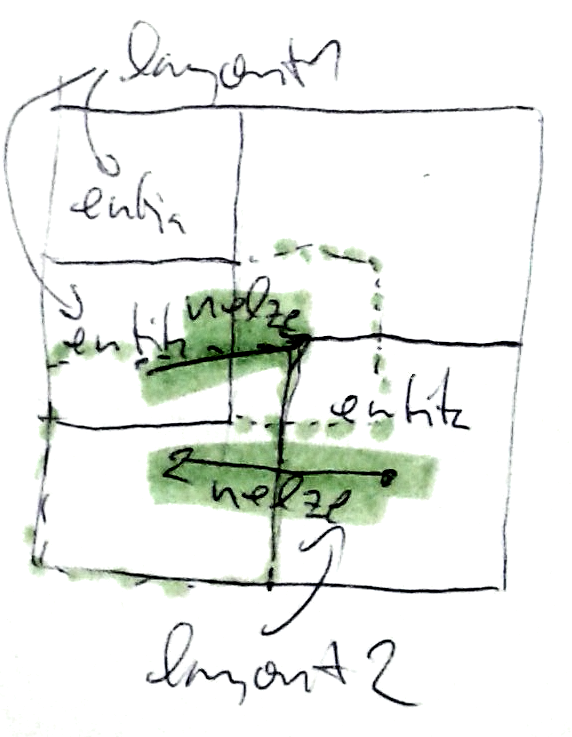
\includegraphics[width=\textwidth]{./img/layout-manager.png}
\caption{Ilustrace vlastností prostorů. }
\label{layout-manager}
\end{figure}



\subsection{Relace s dalšími entitami}

Každá živá entita musí definovat vlastnost typu \ccc{IRelationManager}. Toto rozhraní musí definovat relační token typu
\ccc{RelationToken} pro danou entitu. Dále definuje funkce, která pro daný token vrátí, zda entity odpovídající danému 
tokenu je nepřátelská. Jednoduchou implementací tohoto rozhraní je třída \ccc{DefaultRelationManager}, která má
si při svém vzniku definuje své neměnné nepřátelé. Nicméně pokud daná implementace nevyhovuje je čistě na programátorovi,
aby si vytvořil implementaci vlastní. K dispozici je ještě generátor unikátních tokenů a to statická třída \ccc{RelationTokenFactory}.

\subsection{Implementace entit}
Engine obsahuje implementaci dvou entit a to pro šampiony jejich nepřátele.

\subsubsection{Šampion}
Šampion je první živá
entita a reprezentuje jej třída \ccc{Champion}. Šampion neobsahuje žádnou umělou inteligenci, je ovládán hráčem skrze
třídu \ccc{Leader}, která reprezentuje hráčovu skupinu šampionů. Inicializace vlastností a schopností probíhá přes
datový initializer definovaný rozhraním \ccc{IChampionInitializer}. Resp. jeho předáním do konstruktoru, dále je nutné
specifikovat relační token a seznam nepřátel. Posunout daného šampiona je možné přiřazením do vlastnosti \ccc{Location}.

Zde je dobré zmínit generickou třídu \ccc{Animator}, která má dva typové parametry. První z nich je typ posouvaného 
objektu, který musí implementovat alespoň rozhraní \ccc{IMovable}. Toto  rozhraní definuje vlastnosti, pomocí kterých lze měnit
pozice daného objektu. Dalším parametrem je typ prostorů, mezi kterými se objekt pohybuje. Ten musí implementovat alespoň 
rozhraní \ccc{IStopable}, které definuje pozici, na kterém se má objekt postavit. Animátor poskytuje API pro plynulý
posun objektů mezi prostory.

U šampiona je tento animátor použit automaticky při změně lokace.

\subsubsection{Nepřátelské entity}
Nepřátele reprezentuje třída \ccc{Creature}. Tato třída reprezentuje všechny 
příšery ve hře. Vlastnosti jednotlivých typů příšer jsou ve třídách typu \ccc{CreatureFactory}. Každá konkrétní instance 
příšery má referenci na tuto třídu a její chování je ovlivněné vlastnostmi v ní obsažené. 

Tato třída definuje pro příšery jednoduchou umělou inteligenci. K zjednodušení implementace jsou zde využity 
asynchronní funkce. Ty jsou především využity pro vytváření zpoždění akcí pomocí \ccc{Task.Delay}, bez nutnosti počítání času a vracení se zpět
do funkce po jeho uplynutí. Důležité je poznamenat, že asynchronní funkce jsou prováděny v jednom vlákně a to vždy ve funkci \ccc{Update}. V každém volaní funkce
je vyprázdněna celá fronta asynchronních funkci, proto je třeba dávat pozor na její přehlcení, které může v konečném důsledku vést až k neresponzivnosti aplikace.
Následuje seznam funkcí a jejich popis použitých pro simulování inteligence. Všechny tyto funkce je možné přetěžovat.
\begin{itemize}

\item \ccc{Live} - V této funkci je nekonečný cyklus, který volá obslužné rutiny podle stavu příšery. Jsou to:
	\begin{itemize}
    \item Lov - příšera spatřila nepřítele a pronásleduje ho 
    \item Cesta domů - příšera pronásledovala nepřítele, kterého následně ztratila, proto jde domů tj. na místo svého vzniku
    \item Hlídkování - příšera hlídkuje v okolí oblasti svého vzniku
	\end{itemize}

\item \ccc{FindEnemies} - Pomocí prohledávání do šířky se pokusí najít entity s nepřátelským tokenem. Maximální hledanou oblast
je určena dle vlastností příšery. Pokud je nepřítel nalezen nastaví proměnou \ccc{hountingPath}.

\item \ccc{MoveToSpace} - Přesune příšeru mezi prostory pomocí animátoru a nastaví správně použité prostory pomocí \ccc{LayoutManageru}.

\item \ccc{MoveThroughSpaces} - Přesune příšeru přes prostory dlaždice až na cílovou dlaždici pomocí funkce \ccc{MoveToSpace}. Při každém pohybu hledá nepřátele
pomocí funkce \ccc{FindEnemies}, pokud je tak nastaveno parametrem funkce. Pokud nějaké najde, přeruší pohyb.

\item \ccc{MoveToNeighbourTile} - Posune příšeru na určenou dlaždici přes prostory dlaždice pomocí funkce \ccc{MoveThroughSpaces}.
 Pokud je cesta nepřístupná vrátí \ccc{false}.

\item \ccc{GoHome} - Příšera jde domů podle cesty uložené v proměnné \ccc{homeRoute} a poté ji nastav na \ccc{null}. 
         Mezi dlaždicemi se posunuje pomocí funkce \ccc{MoveToNeighbourTile}.

\item \ccc{FindNextWatchLocation} - Pomocí prohledávání do šířky z místa objevení příšery nalezne dlaždici, na které dlouho
příšera nebyla a vrátí k ní cestu.

\item \ccc{WatchAround} - Pomocí funkce \ccc{FindNextWatchLocation} nalezne cestu na další místo k hlídkování. Poté jde na dané místo
 pomocí funkce \ccc{MoveToNeighbourTile}.

\item \ccc{Fight} - Provede útok na nepřítele.

\item \ccc{PrepareForFight} - Dostane se co nejblíže k dlaždici, na který je nepřítel a zahájí útok pomocí funkce \ccc{Fight}.

\item \ccc{GetPathHome} - Pokusí se nalézt cestu domů. Pokud ji nalezne nastaví \ccc{homeRoute}.

\item \ccc{EstablishNewBase} - Nastaví výchozí dlaždici na nynější.

\item \ccc{Hount} - Příšera pronásleduje nepřítele na poslední místo, kde ho spatřila. Pokud je nepřítel na sousední dlaždici připraví
se k útoku pomocí funkce \ccc{PrepareForFight}. Pokud nepřítele ztratí, pokusí se najít cestu domů pomocí \ccc{GetPathHome}. Pokud
cestu nenalezne založí si domov tam, kde je pomocí funkce \ccc{EstablishNewBase}.

\end{itemize}

K prohledávání do šířky se používá třída \ccc{BreathFirstSearch} nebo některý její potomek. 

\section{Předměty}
Předměty reprezentuje rozhraní \ccc{IGrabableItem}. Jak již bylo zmíněno v analýze\vref{item-factories}, každý předmět musí mít referenci na svoji 
továrnu minimálně typu \ccc{IGrabableItemFactoryBase}. Dále musí definovat vlastnost \ccc{Location} určující prostor dlaždice, na kterém se nachází. 
Přiřazení do této vlastnosti by mělo vyvolat přidání daného předmětu na danou dlaždici. Existují i případy, kdy toto není 
žádoucí a proto předměty musí ještě definovat funkci \ccc{SetLocation}, která pouze danou vlastnost nastaví. V poslední řadě musí definovat renderer.

Rozhraní továrny na obecné předměty vyžaduje vlastnosti jako název, hmotnost, seznam 
možných akcí s předmětem a také definuje místa, kam lze předmět uložit.

\subsection{Implementace předmětů}
Při tvorbě vlastního předmětu je třeba vytvořit implementaci zmíněného rozhraní \ccc{IGrabableItem}. Tato implementace by 
kromě vyžadovaných položek měla obsahovat položky, které se můžou měnit pro každou instanci daného typu předmětu. 
Dále je třeba vytvořit samotnou továrnu na tyto předměty implementací rozhraní \ccc{IGrabableItemFactory}.
Ta by měla obsahovat všechny společné vlastnosti pro daný typ předmětu. Z toho  důvodu je dobré do vlastností 
přidat kromě rozhraním požadované reference na továrnu i přesně typovanou referenci, skrze kterou bude možné k 
vlastnostem přistupovat. Podobnou věc je dobré udělat i v továrně pro funkci vytvářející daný objekt. Inspirace
lze nalézt v již implementovaných třídách, které jsou v jemném prostoru \ccc{DungeonMasterEngine.DungeonContent.GrabableItem}.

\section{Akce}
TODO
\section{Kouzla}
TODO

\section{Renderery}
Jak bylo zmíněno v analýze engine odděluje zobrazovací vrstvu od zbytku enginu\vref{renderer-interactor}. Všechny objekty,
které potřebují mít grafický výstup by měli implementovat rozhraní \ccc{IRenderable}, které vyžaduje položku typu \ccc{IRenderer}. 
Stěžejní funkce tohoto rozhraní jsou funkce \ccc{Render} a \ccc{Interact}. 

Nejdůležitější z parametrů těchto funkcí je dosavadní transformace. Tj. obsahuje složeninu transformací složenou z jednotlivých
transformací na cestě z kořene stromu reprezentující závislosti rendererů na sobě. Takže například kořen stromu bude renderer
dlaždice, jeho syn bude strana dlaždice, její syn bude výklenek ve zdi a její syn bude předmět ve
výklenku(list). Při takovéto reprezentaci se pak musí všechny renderované objekty posunout či jinak transformovat vůči jejich rodiči.
Tzn. každý renderer si musí zvolit pozicovací konvenci, kterou pak musí závislé renderery dodržovat. Tento způsob renderování je požíván u statických objektu jako
jsou dlaždice, stěny, výklenky a podobně. Pro pohybující objekty je používaná absolutní pozice a renderery
těchto objektů transformují objekty přímo na jejich pozici. Volba mezi těmito dvěma způsoby pozicování stojí vždy z zamyšlení.

Renderery jsou vždy dělány na míru objektu, který mají renderovat. Tzn. často se renderer v konstruktoru 
inicializuje instancí s konkretním typem. Třída této instance pak má zpravidla readonly vlastnosti,
podle kterých renderer určuje, co má vykreslovat. Jelikož implementovaná grafická vrstva je pouze ve formě proof of concept,
je co nejjednodušší a neobsahuje například animace. Nicméně ze zde popsané povahy rendererů je jasné, že 
toho může být dosaženo vytvořením událostí na renderovaných objektech, které si renderer zaregistruje.
Dovedeme si představit, že by šla s takovým návrhem velmi jednoduše udělat grafická vrstva, která bude
velmi pěkná, bude mít kvalitní 3D modely a animace. Zabralo by to jen spoustu času a byla by k tomu potřeba spousta grafiků.

Při rozšíření nějakého rendereru je třeba zjistit dosavadní transformaci, která je normálně vypočítána v rodiči.
K tomuto záměru slouží funkce \ccc{GetCurrentTransformation}, která bere jako parametr dosavadní transformaci.
Rozšířením jež existujícího rendereru si lze ušetřit mnoho práce a opakujícího se kódu. Proto je takový přístup v této implementaci často použit.
Funkce popsané na začátku sekce jsou samozřejmě virtuální a jdou přetěžovat,
obsahují také jeden parametr typu \ccc{object} pro případné předávaní dodatečných dat mezi renderery. Tohoto parametru není nikde v této implementaci využito.

Jelikož renderery zásadně mění vzhled a pozici všech věcí, je nutné tuto vrstvu propojit i s interakcí.
Interakční funkce má skrze parametr typu \ccc{ILeader}  přístup k položce interactor, která je typu \ccc{object}.
Daný renderer musí vědět, pro jaký typ interactoru je a na ten si ho musí vhodně přetypovat. V této implementaci je použit paprsek (\ccc{Ray}). 
Celý tento koncept interactoru by šel sice udělat genericky, ale prolínal by se celou strukturou rendererů a z toho
důvodu jsem se rozhodl v tomto místě ustoupit a udělat situaci jednoduší na úkor kontroly za překladu.

\section{Builder map}
Nyní když máme rozebrané všechny části enginu, které je potenciálně možné rozšířit, si můžeme vysvětlit, jak
se vše sestaví dohromady v herní úroveně.

\subsection{Vlastní implementace builderu}
Jak již bylo zmíněno builder musí implementovat rozhraní \ccc{IDungeonBuilder}\vref{engine-core}. Toto rozhraní je
potom dotazované pro načtení herní úrovně jádrem enginu. Je úkolem builderu rozhodnout jak bude jednat
v případě, že je podán několikrát dotaz na stejnou mapu. Typicky je se tedy nutné rozhodnout
jestli načtené mapy kešovat či nikoliv. 

Správně implementovaný builder by měl načítat mapy zhruba tímto způsobem. 

\begin{enumerate}

\item Vytvoření dlaždic a naplnění jejich inicializátorů. 
To znamená vytvořit strany dlaždic a přepínače či předměty v nich obsažené.

\item Nastavení sousedů dlaždic do inicializátorů. 

\item Vytvoření samotného levelu \ccc{DungeonLevel}.

\item Dokončení inicializace inicializátoru a zavolaní inicializaci dlaždic skrze inicializátory. 

\item Případné kešování herní úrovně pro případný opakovaný požadavek. 
\end{enumerate}

Na tyto body se samozřejmě navazuje spoustu další věcí, které je třeba vyřešit. 
Je to například vytvoření továren pro akce a předměty. Továrny pro akce jsou pak použity pro
továrny pro předměty a ty zase pro vytvoření samotných předmětů. 

 Dále je potřeba vyřešit 
nastavení rendererů. Pokud má builder podporovat různé zobrazovací vrstvy, je potřeba 
nějakým způsobem poskytnout možnost předání jiných rendererů builderu. Je tedy například
možné vytvořit rozhraní, které bude vracet dané renderery používané v builderu. Odlišnou
implementaci rozhraní se potom budou požívat odlišné renderery.


\subsection{Implementace builderu Dungeon Masteru}
Builder pro samotnu hru Dungeon Master řeší třída \ccc{LegacyMapBuilder}. Tento builder
využívá již rozparsovaná data reprezentována třídou \ccc{DungeonData}.
Samotný builder map potom využívá ještě další buildery. Jsou to třídy pro vytváření
dlaždic, přepínačů, předmětů a příšer. Při požadavku na určitou mapu pak 
následuje postup zmíněný v předchozí sekci.

\chapter{Uživatelská dokumentace}
Tento projekt si neklade za cíl udělat zcela kompletní a dobře hratelnou reimplementaci Dungeon Master.
Naopak se soustředí na dobrý návrh enginu jako takového. Z toho důvodu není herní zážitek nikterak
oslňující, nicméně jako demonstrace funkčnosti enginu poslouží dobře. Hru je možné spustit souborem
\ccc{DungeonMasterEngine.exe}.

\section{Mechaniky ve hře}
Hráč reprezentuje vůdce skupiny bojovníků známých jako šampióni. Může ovládat jejich pohyb, 
předávat jim předměty, donutit je k boji, ke kouzlení, ke konzumaci jedlých předmětů nebo lektvarů.
Každý bojovník má sadu vlastností a schopností, v kterých je schopný se zdokonalovat získáváním zkušeností.
Zkušenosti lze získat bojem na prázdno, bojem proti příšerám, kouzlením, nebo jen použitím přepínačů.
V dungeonu jsou přepínače na zdích, které lze aktivovat kliknutím myši. Dále jsou zde přepínače na 
podlaze, které lze aktivovat vstoupením na podlahu nebo hozením předmětu na daný spínač. Předměty lze
pokládat na zem, do výklenků a nebo je uložit na tělo bojovníka či do jeho batohu. Přepínače pak mohou 
aktivovat nebo deaktivovat určité objekty ve hře jako jsou například dveře, teleporty, jámy, otevírací
zdi atp. Některé dveře je také možné rozbít útkem. Některé teleporty jsou pouze na konkrétní typy objektů.
Do jam lze spadnout, ale většinou se z nich lze právě teleportem dostat ven.


\section{Cíl hry}
Jak již bylo zmíněno, tak hra není úplně kompletní, proto ji není možné zcela dohrát. Z toho důvodu by se za cíl 
hry dalo považovat dostaní se do posledního implementovaného levelu hry.

\section{Ovládání}

\subsection{Pohyb}
Pohybovat skupinou lze pomocí kláves w,s,a,d tj. dopředu, dozadu, doleva, doprava. Dále se je možné rozhlížet pomocí šipek.

\subsection{Aktivace přepínačů a sbírání předmětů}
Přepínače lze aktivovat namířením ukazatele myši na daný objekt a kliknutím nebo stiskem klávesy \ccc{ENTER}. Pokud
se pod kurzorem vyskytuje předmět nebo  přepínač, který může vložit nějaký předmět hráčovi do ruky, tak se tak provede pokud je
hráčova ruka prázdná. Pokud hráč již v ruce něco má, provede se opačná akce tj. předmět se položí na dané místo nebo je 
pohlcen přepínačem. Ostatní interakce probíhá přes konzoli. Konzole se aktivuje stiskem klávesy \ccc{TAB} a deaktivuje opětovným
stisknutím tytéž klávesy. Příkaz \ccc{hand} zobrazí popis předmětu v hráčově ruce. Přidáním parametru \ccc{take} se provede
uložení předmětu do dotazovaného inventáře daného bojovníka. Přidáním parametru \ccc{put} se naopak vloží dotazovaný objekt z inventáře
do ruky.

\subsection{Souboj}
Pro souboj je nejprve nutné vložit zbraň to akční ruky. Což je možné provést příkazy z minulé sekce.
Samotný souboj probíha potom skrze příkaz \ccc{fight}, kdy je interaktivně vybrán bojovník a způsob útoku.

\subsection{Konzole}
Pro více informací o příkazech je možné napsat příkaz \ccc{help} do konzole.

\chapter*{Závěr}
\addcontentsline{toc}{chapter}{Závěr}

V rámci této práce byl naimplementovaný engine pro Hru Dungeon Master. Engine 
obsahuje podporu pro všechny funkce z originální hry. Nicméně všechny konkrétní funkce
nejsou naimplementované do úplných detailů, což dává možnost navázat na práci případným následovníkům. 
 Pro implementaci byl použit jazyk C\#, platforma .NET
a framework MonoGame. Většina částí enginu je jednoduše rozšiřitelná či modifikovatelná.
To vede na dobrou udržitelnost celého systému. Primárně je engine určený pro hru 
Dungeon Master a dokáže si herní úrovně načíst z originální binárních dat. Nicméně
načítání map je v oddělené vrstvě a proto je možné tuto vrstvu upravit kvůli případným rozšířením nebo ji je možné
nově naimplementovat i pro 
jiné vstupní formáty. Z toho důvodu je možné tento engine využít i pro implementaci jiných her na podobných principech.
Engine má také oddělenou renderovací vrstvu, která lze jednoduše upravit dle potřeby.



